\documentclass[12pt]{article}
\usepackage{hyperref}
\usepackage{comment}
\usepackage{import}
\import{}{ThesisCommands}
\bibliographystyle{alpha}
\newcommand{\M}{\mathcal{M}}


\usepackage{fancyhdr}
\usepackage{extramarks}
\pagestyle{fancy}
\renewcommand{\sectionmark}[1]{\markright{\thesection\ #1}}
\fancyhf{}
\fancyhead[LO]{\textbf{\rightmark}}

\rfoot{Page \thepage}
\renewcommand{\headrulewidth}{1pt}
\renewcommand{\footrulewidth}{0.5pt}


\begin{document}


%----------------------------------------------------------------------------------------
%	TITLE PAGE
%----------------------------------------------------------------------------------------

\begin{titlepage} % Suppresses headers and footers on the title page
	
	\centering % Centre everything on the title page
	
	%------------------------------------------------
	%	Top rules
	%------------------------------------------------
	
	\rule{\textwidth}{1pt} % Thick horizontal rule
	
	\vspace{2pt}\vspace{-\baselineskip} % Whitespace between rules
	
	\rule{\textwidth}{0.4pt} % Thin horizontal rule
	
	\vspace{0.1\textheight} % Whitespace between the top rules and title
	
	%------------------------------------------------
	%	Title
	%------------------------------------------------
	
		{\Huge CURVES ON TORIC SURFACES}\\[0.5\baselineskip] % Title line 1
		{\Large AND THEIR}\\[0.5\baselineskip] % Title line 2
		{\Huge REGULAR MODELS} % Title line 3
	
	\vspace{0.025\textheight} % Whitespace between the title and short horizontal rule
	
	\rule{0.3\textwidth}{0.4pt} % Short horizontal rule under the title
	
	\vspace{0.1\textheight} % Whitespace between the thin horizontal rule and the author name
	
	%------------------------------------------------
	%	Author
	%------------------------------------------------
	
	{\Large \textsc{Benjamin Church}} % Author name
	
	\vfill % Whitespace between the author name and publisher
	
	%------------------------------------------------
	%	Publisher
	%------------------------------------------------

	{\Large\textsc{Columbia University}} % Publisher
	\\
	{\large\textsc{undergraduate thesis}}
	
	\vspace{0.05 \textheight}
	
	{\textsc{supervised by:}}
	\\
	{\large\textsc{Aise Johan de Jong}}
	
	\vspace{0.1\textheight} % Whitespace under the publisher text
	
	%------------------------------------------------
	%	Bottom rules
	%------------------------------------------------
	
	\rule{\textwidth}{0.4pt} % Thin horizontal rule
	
	\vspace{2pt}\vspace{-\baselineskip} % Whitespace between rules
	
	\rule{\textwidth}{1pt} % Thick horizontal rule
	
\end{titlepage}

\section{Introduction}

The theory of regular or, more generally, semistable models for smooth proper curves provides a bridge between the behavior of classical ``geometric'' curves and certain arithmetic phenomena and counting problems which occur for curves over finite fields. The problem of computing models for curves traces back to the notion of reduction modulo $p$ of elliptic curves developed to link the global Hasse-Weil zeta function to local zeta functions even at primes of ``bad reduction.'' A full classification of degenerate fibers occurring in minimal elliptic fibrations was carried out by Kodaira \cite{kodaira} which labeled degenerations by Dynkin diagrams and Kodaira types. Furthermore, Tate's algorithm \cite{tate} solves the problem of computing the reduction types and semistable models at a prime for elliptic curves defined over number fields.
\par
There is, however, no known general algorithm to produce regular models of higher genus curves. Recent results of \cite{tim} construct the minimal normal crossing model of curves satisfying a certain regularity condition. This condition is generic on the moduli of plane affine equations but \textit{not general} on the moduli space of sufficiently-high genus curves. The construction and regularity condition heavily employs the methods of toric geometry and the theory of toric compactification of curves.
\par
We show that a generic curve is not toric and thus cannot satisfy the regularity condition of \cite{tim}. Furthermore, even among toric curves, we provide examples demonstrating arithmetic phenomena which may arise in minimal models and which cannot be captured in the aforementioned toric construction. In preparation, we review toric geometry, discuss the generalities of embedding curves in toric surfaces with an eye towards combinatorial descriptions, and give a proof of Baker's theorem relating the genus to counting lattice points using an adjunction sequence.

\subsection{Conventions and Basic Definitions}

All rings are assumed to be commutative and unital and ring maps are required to preserve the unit. We make no assumption that in a ring $0 \neq 1$ so the category of rings has a final object, the zero ring denoted as $0$. We make widespread use of the standard language and terminology of scheme theory as developed in \cite{har} or \cite{EGA}. Throughout, we say a \textit{variety} is an integral separated scheme of finite type over a field $k$, a \textit{curve} is a dimension one variety, and a \textit{surface} is a dimension two variety. However, in the discussion of models over a discrete valuation ring $R$, we will have dimension two schemes $X \to \Spec{R}$ which we may refer to as \textit{arithmetic surfaces} although they are not, strictly speaking, surfaces in the prior sense. Often, in practice, our varieties will be geometrically integral but we make no general assumption that this is so and will give explicit hypotheses when such conditions are necessary. Finally, regarding our conventions for toric geometry, we make the semi-standard requirement that toric varieties be \textit{normal}. Note this does not agree with Cox \cite{cox, cox_lectures}, our chosen standard reference for all things toric, who allows non-normal toric varieties. For example, there is some debate whether the rational curve $V(X^3 - Y^2 Z) \subset \P^3_k$ ought to be considered a toric variety \cite[Lec. 1, Ex. 1.4]{cox_lectures}. We believe the normality hypothesis is satisfactory because it gives the theory a coherent combinatorial picture in terms of real convex lattice geometry which will be desirable for our interests.

\subsection{Acknowledgments}

I would like to thank Aise Johan de Jong for advising this project and for consistently giving me thoughtful comments and explanations. My sincerest gratitude goes out to Raymond Cheng for his continual aid, enthusiasm, and patience over the last three years. I am deeply indebted for his assistance and encouragement in all things mathematical. I would also like to thank Michael Harris, Huayi Chen, Raymond Cheng, and the other teachers and organizers of the 2019 Columbia - Paris Diderot REU which ignited my study of toric geometry. Finally, I would like to thank Vesna Gasperov for her guidance as well as the Columbia SRF program for funding my summer studies. 

\tableofcontents
\newpage

\section{A Brief Review of Toric Geometry}

\begin{defn}
A \textit{toric variety} $X$ is a normal variety over $k$ with a dense open embedding of the torus $\T^n = (\Gm{k})^n \embed X$, where $n = \dim{X}$, such that the natural action of the torus on itself as a group scheme extends to an action $\T^n \times X \to X$. 
\end{defn}

\begin{rmk}
Any toric variety is rational. A birational map $\P^n_k \birat X$ is induced by the inclusion of the torus $\Gm{k}^n \embed X$ which is a dense open immersion and thus gives an isomorphism between dense open subsets of $\P^n_k$ and $X$.
\end{rmk}


\subsection{The Toric Variety Associated to a Fan}

Our notation here follows Cox's text and lectures \cite{cox,cox_lectures} for the discussion of the objects of combinatorial geometry and their corresponding toric data.

\begin{defn}
Here we fix a lattice $N$ and let $M$ denote its dual lattice with the canonical pairing $\inner{}{} : M \times N \to \Z$. Then $N_\R = N \otimes_\Z \R$ and $M_\R = M \otimes_\Z \R = (N_\R)^*$. We define the following convex geometric objects,
\begin{enumerate}
\item a \textit{cone} $\sigma \subset N_\R$ is a subset closed under addition and positive scaling by $\R^+$,
\item a \textit{convex polyhedral cone} is a cone $\sigma \subset N_\R$ which is generated by a finite set $\sigma = \Cone{v_1, \dots, v_n }$ for $v_1, \dots v_n \in N_\R$,
\item a \textit{rational polyhedral cone} is a cone $\sigma \subset N_\R$ such that $\sigma = \Cone{S}$ for a finite set $S \subset N$ i.e. $\sigma$ is generated by a finite number of integral lattice points,
\item $\dim{\sigma} := \dim{\vspan{\sigma}}$.
\end{enumerate}
\end{defn}

\begin{defn}
Given a cone $\sigma \subset N_\R$ we define the \textit{dual cone},
\[ \sigma^\vee = \{ m \in M \mid \forall n \in \sigma : \inner{m}{n} \ge 0 \} \]
and the \textit{associated monoid},
\[ S_\sigma = \sigma^\vee \cap M \]
\end{defn}

\begin{lemma}[Gordan]
If $\sigma \subset N_\R$ is a rational polyhedral cone then $S_\sigma = \sigma^\vee \cap M$ is a finitely generated monoid. 
\end{lemma}

\begin{proof}
\cite[Prop. 1.2.17]{cox}.
\end{proof}

\begin{defn}
A cone $\sigma \subset N_\R$ is called \textit{strongly convex} if it satisfies one of the following equivalent conditions,
\begin{enumerate}
\item $\sigma \cap (-\sigma) = \{ 0 \}$,
\item $\dim{\sigma^\vee} = n$,
\item $\{ 0 \}$ is a face of $\sigma$,
\item $\sigma$ contains no positive-dimensional vector spaces.
\end{enumerate}
\end{defn}

\begin{defn}
Let $k$ be a field and $S$ a monoid. Then the monoid algebra $k[S]$ is generated by monomials of the form $\chi^m$ for $m \in S$ satisfying $\chi^{m_1 + m_2} = \chi^{m_1} \cdot \chi^{m_2}$. 
Alternatively, the functor $k[-] : \mathbf{CMon} \to \Alg_k$ is left-adjoint to the forgetful functor via,
\[ \Homover{k}{k[S]}{A} = \Homover{\mathbf{CMon}}{(S, +)}{(A, \times)} \]
Thus $k[S]$ represents the functor $\Alg_k^\op \to \Set$ sending $S \mapsto \Hom{\mathbf{CMond}}{(S, +)}{(A, \times)}$.
\end{defn}

\begin{defn}
Let $\sigma \subset N_\R$ be a strongly convex rational polyhedral cone. Then the associated affine toric variety is,
\[ U_\sigma = \Spec{k[S_\sigma]} = \Spec{k[\sigma^\vee \cap M]} \]
with torus $\Spec{k[M]} \to \Spec{k[S_\sigma]}$ via $S_\sigma \subset M$ and thus $k[S_\sigma] \embed k[M]$ is a localization map since $\dim{\sigma^\vee} = n$. Furthermore, choosing $M \cong \Z^n$,
\[ \Spec{k[M]} = \Spec{k[\Z^n]} = \Gm{k}^n \]
\end{defn}

\begin{theorem}
Let $U$ be an affine toric variety. Then $U = \Spec{k[S_\sigma]}$ for some strongly convex rational polyhedral cone $\sigma$.
\end{theorem}

\begin{proof}
See \cite[Thm. 1.3.5]{cox}.
\end{proof}

\begin{rmk}
The equivalence between affine toric varieties and convex polyhedral cones holds since we require toric varieties to be normal. Without this assumption, an affine toric variety may be generated by a non-saturated monoid (e.g. \cite[Ex. 1.10]{cox_lectures}).
\end{rmk}

\begin{remark}
If $\tau$ is a face of $\sigma$ then $S_\tau \supset S_\sigma$ induces $k[S_\sigma] \to k[S_\tau]$ and thus a morphism $U_\tau \to U_\sigma$. The map $U_\tau \to U_\sigma$ is an open embedding because $k[S_\sigma] \to k[S_\tau]$ is a localization. 
\end{remark}

\begin{definition}
A \textit{fan} is a finite collection $\Sigma$ of strongly convex rational polyhedral cones in $N_\R$ such that,
\begin{enumerate}
\item $\forall \sigma \in \Sigma$ and any face $\tau$ of $\sigma$ then $\tau \in \Sigma$,
\item $\forall \sigma, \tau \in \Sigma$ the intersection $\sigma \cap \tau$ is a common face of $\sigma$ and $\tau$ and $\sigma \cap \tau \in \Sigma$.
\end{enumerate}
Given a fan $\Sigma$ we define the sets,
\[ \Sigma(k) = \{ \sigma \in \Sigma \mid \dim{\sigma} = k \} \]
\end{definition}

\begin{remark}
The smallest face of a fan $\Sigma$ is $\{ 0 \}$ for which $\{ 0 \}^\vee = M$ thus defining the embedded torus,
\[ U_{\{0\}} = \Spec{k[M]} \cong \Spec{k[\Z^n]} = \mathbb{G}_{m,k}^n \]
\end{remark}

\begin{remark}
If $\sigma$ and $\tau$ intersect in a common face $S_{\sigma \cap \tau} = S_\sigma + S_\tau$ then the embeddings $U_{\sigma \cap \tau} \to U_{\sigma}, U_{\tau}$ allow gluing. 
\end{remark}


\begin{definition}
Given a fan $\Sigma$ we define the toric variety $\Toric_\Sigma$ via gluing $U_\sigma$ for each $\sigma \in \Sigma$ under the inclusions,
\begin{center}
\begin{tikzcd}
U_\sigma & &  U_\tau
\\
& U_{\sigma \cap \tau} \arrow[ru] \arrow[lu]
\end{tikzcd}
\end{center}
The affine toric varieties $U_{\sigma}$ form a diagram on the inclusion poset of $\Sigma$. This gluing data defines a variety $\Toric_\Sigma$ over $k$.
\end{definition}

\begin{rmk}
The torus embedding is given by the cone $\sigma = \{ 0 \}$ which corresponds to an open $U_\sigma = \Spec{k[M]} \embed \Toric_\Sigma$. Furthermore, $T_\Sigma$ is normal because the cover of affine opens $U_{\sigma} = \Spec{k[\sigma^\vee \cap M]}$ because $k[\sigma^\vee \cap M]$ is an integrally closed domain since $\sigma^\vee \cap M \subset M$ is a saturated submonoid (see \cite[Thm. 1.14 + Ex. 1.11]{cox_lectures}).
\end{rmk}

\noindent
Finally, we discuss the relationship between the structure of a toric variety defined by a fan and the combinatorial structure of the fan. In particular, the closure of the torus $\T^n$ has interesting structure at infinity which corresponds to the nonzero cones as follows.

\begin{prop}
For each cone $\sigma \in \Sigma$ we define the locally closed subset of $\Toric_\Sigma$,
\[ O(\sigma) : = U_\sigma \setminus \left( \bigcup_{\tau \prec \sigma} U_\tau \right) \]
where $\tau \prec \sigma$ if $\tau$ is a proper face of $\sigma$. This is cut out by ideal $I$ generated by the equations $\chi^m $ for $m \in S_\sigma \setminus \sigma^\perp$ i.e. $O(\sigma) = \Spec{k[S_\sigma]/I}$. Then $O(\sigma) = \T^n \cdot \gamma_\sigma$ is a torus-orbit with a distinguished point $\gamma_\sigma \in U_\sigma$ defined by the maximal ideal $\m_\sigma \subset k[S_\sigma]$ generated by equations,
 \[ \{ \chi^m \mid m \in S_\sigma \setminus \sigma^\perp \} \cup \{ \chi^m - 1 \mid m \in S_\sigma \cap \sigma^\perp \}  \]
\bigskip\\
Furthermore, let $V(\sigma) = \overline{O(\sigma)}$ then $V(\sigma)$ is the toric variety corresponding to the lattice $N / N_\sigma$ where $N_\sigma = \mathrm{Span}(\sigma \cap N)$ with fan $\Sigma_\sigma \subset (N/N_\sigma) \otimes_\Z \R$ which has cones,
\[ \Sigma_\sigma \leftrightarrow \mathrm{Star}(\sigma) = \{ \tau \in \Sigma \mid \tau \supset \sigma \} \]
\[ \bar{\tau} = (\tau + (N_\sigma)_\R)/ (N_\sigma)_\R \subset N_\R / (N_\sigma)_\R = (N/ N_\sigma)_\R \]
where the torus of $V(\sigma)$ is $O(\sigma) = U_{\bar{\sigma}} = \Spec{k[N/N_\sigma]} \cong \Gm{k}^{n - \dim{\sigma}}$ whose closed points are naturally isomorphic to $T(N/N_\sigma) = (N / N_\sigma) \otimes_\Z k^\times$. 
\end{prop}

\begin{proof}
See \cite[Lec. 2]{cox_lectures}.
\end{proof}

\begin{example}
Take the standard fan,
\[ \Sigma = \{ \Cone{s_{1} e_{i_1}, \dots, s_k e_{i_k}} \mid i_1, \dots, i_k = 1, \dots, n \quad s_i = \pm 1 \quad k = 0,1,\dots, n \} \] where $\{ e_i \}$ is the standard basis of $\Z^n \subset \R^n$. Then,
\[ U_\sigma = \Spec{k[x_{i_1}^{s_i}, \dots, x_{i_k}^{s_k}, (x^{\pm 1}_{j})_{j \neq i_1, \dots, i_k}]} \]
Thus $O(\sigma)$ is the locus where $x_{i_1}, \dots, x_{i_k}$ vanish.
Furthermore, the distinguished point $\gamma_\sigma$ is the closed point where $x_{i_1} = \cdots = x_{i_k} = 0$ and $x_j = 1$ for $j \neq i_1, \dots, i_k$. The toric variety associated to this fan is $\Toric_{\Sigma} = (\P^1_k)^n$ with $x_i$ being the affine coordinate $\frac{T_1}{T_0}$ on $\P^1_k = \Proj{k[T_0, T_1]}$.
\end{example}

\begin{theorem}[Cone-Orbit Correspondence]
There is a correspondence between cones and orbits,
\begin{enumerate}
\item $\{ \text{cones } \sigma \in \Sigma \} \leftrightarrow \{ \Toric^n \text{ - orbits of } \Toric_\Sigma \}$ via $\sigma \mapsto O(\sigma)$ is a bijection
\item $\dim{\sigma} + \dim{O(\sigma)} = n$
\item $O(\tau) \subset \overline{O(\sigma)} \iff \sigma \subset \tau$
\end{enumerate}
and an inclusion-reversing correspondence between cones are torus-invariant closed subvarieties,
\begin{enumerate}
\item $\{ \text{cones } \sigma \in \Sigma \} \leftrightarrow \{ \Toric^n \text{- invariant closed subvarieties of } \Toric_\Sigma \}$ via $\sigma \mapsto V(\sigma)$ is a bijection
\item $\dim{\sigma} + \dim{V(\sigma)} = n$
\item $V(\tau) \subset V(\sigma) \iff \sigma \subset \tau$.
\end{enumerate}
In particular, for each $\sigma$ there is a partition,
\[ V(\sigma) = \bigcup_{\tau \supset \sigma} O(\tau) \]
\end{theorem}

\begin{proof}
See \cite[Lec. 2]{cox_lectures}.
\end{proof}

\begin{rmk}
We say that $D_\Toric = \Toric_\Sigma \setminus \Toric$ is the toric divisor of $\Toric_\Sigma$ which is $\Toric$-invariant and,
\[ D_\Toric = \bigcup_{\sigma \neq \{0\}} V(\sigma) = \bigcup_{\sigma \neq \{0\}} O(\sigma) \]
so $D_\Toric$ is a union of toric varieties.
\end{rmk}


\subsection{Smoothness and Singularities of Toric Varieties}

\begin{lemma}
The affine toric variety $U_\sigma$ of a cone $\sigma \subset N \otimes_\Z \R$ is smooth if and only if $\sigma \cap N$ has a minimal generating set which can be extended to a basis of the lattice $N$.
\end{lemma}
\noindent
This observation motivates the following definition:

\begin{defn}
We call a rational polyhedral cone $\sigma \subset N \otimes_\Z \R$ \textit{smooth} if it has a n minimal integral generating set of $\sigma \cap N$ which is a subset of a basis of the lattice $N$. Otherwise we say that $\sigma$ is \textit{singular}.
\end{defn}


\begin{example}
The cone $\sigma = \Cone{(1, 0), (0, 1)}$ is smooth since it is generated by a basis of $\Z^2$. However, $\Cone{(1, 0), (2, 3)}$ is not smooth because these are the minimal integral generators and they do not form a basis of the lattice $\Z^2$ since $(0, 1)$ is not in their $\Z$-span.
\end{example}

\begin{lemma}
The singular locus of the toric variety $\Toric_\Sigma$ associated to a fan $\Sigma$ in terms of the singular cones,
\[ (\Toric_\Sigma)_{\text{sing}} = \bigcup_{\sigma \in \Sigma \text{ singular}} V(\sigma) \]
and thus conversely the smooth locus is,
\[ \Toric_{\Sigma} \setminus (\Toric_\Sigma)_{\text{sing}} = \bigcup_{\sigma \in \Sigma \text{ smooth}} U_\sigma \] 
\end{lemma}
\noindent
In particular, the toric variety $\Toric_\Sigma$ is smooth iff $\Sigma$ is smooth meaning that every cone $\sigma \in \Sigma$ is smooth. 

\begin{proof}
Notice that, because of the toric action of the orbits $O(\sigma)$, if any point in $O(\sigma)$ is singular then every point will be singular. It is clear that whenever there is an inclusion $\sigma \subset \tau$, if $\sigma$ is singular then so is $\tau$. This implies,
\[ (\Toric_\Sigma)_{\text{sing}} = \bigcup_{\sigma \in \Sigma \text{ singular}} O(\sigma) = \bigcup_{\sigma \in \Sigma \text{ singular}} V(\sigma) \]
since the closures of the orbit $O(\sigma)$ corresponds to taking the union of the orbits corresponding to all cones containing $\sigma$. 
\end{proof}

\begin{rmk}
There is no ambiguity between smoothness and regularity for $\Toric_\Sigma$ even when $k$ is non-perfect. Essentially this is because our construction is stable under base change in the sense that given an extension of fields $k \subset k'$, the toric variety $\Toric_\Sigma'$ associated to the same fan $\Sigma$ but constructed over the field $k'$ is simply $\Toric_\Sigma' = \Toric_\Sigma \times_{k} \Spec{k'}$. Therefore to produce $\Toric_{\Sigma}$, we may always pass to the prime subfield $k_p$ of $k$, over which regularity and smoothness coincide since $k_p$ is always perfect, and finally base change to $k$. Since smoothness is preserved under base change we conclude that the smooth and regular loci of $\Toric_\Sigma$ are identical. 
\end{rmk}

\begin{rmk}
We know that $\Toric_\Sigma$ is normal and thus automatically regular in codimension one by an argument on the affines. It is illustrative to show how the orbit-cone correspondence forces $\Toric_\Sigma$ to be regular in codimension one. The essential observation is that any one-dimensional cone $\sigma \subset N \otimes_\Z \R$ is smooth as follows. Writing the minimal generator in $\sigma \cap N$ as $(a_1, \dots, a_n)$ with $a_i$ totally coprime, meaning they generate the unit ideal in $\Z$. Then $(a_{i})$ forms a row of some matrix $A \in \GL{n}{\Z}$ which exactly shows that $\sigma$ is smooth. Explicitly, can find a matrix $B \in \GL{n}{\Z}$ with $B (a_i) = e_1$ then let $A = B^{-1}$ so $A e_1 = (a_i)$. Therefore, the singular locus,
\[ (\Toric_\Sigma)_{\text{sing}} = \bigcup_{\sigma \in \Sigma \text{ singular}} V(\sigma) \subset \bigcup_{\dim{\sigma} > 1} V(\sigma) \]
is a finite union of closed codimension $>1$ toric components and thus is closed of codimension at least two. For any irreducible codimension one closed subscheme $Z \subset \Toric_\Sigma$ with generic point $\eta$ we cannot have $\eta \in (\Toric_\Sigma)_{\text{sing}}$. Otherwise, $Z \subset (\Toric_\Sigma)_{\text{sing}}$ since it is closed, contradicting the fact that the singular locus has codimension at least two.
\end{rmk}
\noindent
We now summarize the smoothness properties of the toric variety $\Toric_\Sigma$ associated to a fan.

\begin{theorem}
The toric variety $\Toric_\Sigma$ associated to the fan $\Sigma$   is,
\begin{enumerate}
\item normal
\item Cohen-Macaulay
\item smooth exactly when $\Sigma$ is smooth
\item complete exactly when $\Sigma$ is complete i.e. $|\Sigma| = N_\R$. 
\end{enumerate}
\end{theorem}

\begin{proof}
See \cite[Lec. 2, Thm. 2.3]{cox_lectures}.
\end{proof}

\subsection{Toric Divisors}


Let us briefly review our definitions of divisors to clarify notation. Let $\K_X$ be the sheaf of meromorphic functions on $X$ then the sheaf of Cartier divisors is $\shDiv_X = \K_X^\times / \struct{X}^\times$ and a Cartier divisor is a section $D \in H^0(X, \shDiv_X)$. The Cartier class group is,
\[ \CaCl{X} = \coker{(H^0(X, \K_X^\times) \to H^0(X, \shDiv_X))} \] 
A basic cohomology calculation gives a natural embedding $\CaCl{X} \embed \Pic{X}$ which is an isomorphism when $H^1(X, \K_X^\times) = 0$ (in particular when $X$ is integral). When $X$ satisfies the Weil property,
\begin{center}
(W) $X$ is a Noetherian, integral, separated scheme which is regular in codimension one. 
\end{center} 
we define a prime divisor $Z$ on $X$ to be a codimension one integral closed subscheme and a Weil divisor $D \in \Div{X}$ to be a formal (finite) sum of prime divisors of $X$. A principal divisor is of the form $(f) \in \Div{X}$ for $f \in K_X^\times$ where,
\[ \div(f) = \sum_{Z \text{ prime}} \ord_{Z}(f) \: \: [Z] \]
then $\Cl{X}$ is the group of Weil divisors modulo principal divisors. Furthermore, any Weil divisor class injectively defines a coherent sheaf $\struct{X}(D)$ with the following property,
\[ \Gamma(U, \struct{X}(D)|_U) = \{ f \in K(X) \mid \div{(f)} + D \ge 0 \text{ on } U \text{ or } f = 0 \} \] 
There is a canonical embedding $\CaCl{X} \embed \Cl{X}$ which is an isomorphism when $X$ is locally factorial. A Weil divisor is a Cartier divisor (i.e. is in the image of $\CaCl{X} \embed \Cl{X}$) if and only if $\struct{X}(D)$ is invertible which is then the corresponding line bundle under $\CaCl{X} \embed \Pic{X}$.
\begin{rmk}
Note that the map $\struct{X}(D) \otimes_{\struct{X}} \struct{X}(E) \to \struct{X}(D + E)$ given by $f \otimes g \mapsto fg$ is an isomorphism if one of $D$ or $E$ is Cartier but may, in general, fail to be an isomorphism. 
\end{rmk}
\noindent\\
Note that (W) always holds for toric varieties since they are normal varieties. Therefore, in the toric case, we have $\Pic{X} = \CaCl{X} \embed \Cl{X}$ which is an isomorphism when $X$ is smooth. However, toric varieties have a special class of divisors, those which are invariant under the torus action which, for Weil divisors, are exactly generated by prime divisors supported on the toric divisor $D_\T = X \setminus \T^n$. Such prime divisors are exactly the codimension one torus-invariant closed subschemes which, by the cone-orbit correspondence, correspond to $V(\rho)$ for rays $\rho \in \Sigma(1)$. We call these prime advisors $D_\rho = V(\rho)$ for each $\rho \in \Sigma(1)$. The fundamental property of divisors on toric varieties is that any divisor is linearly equivalent to a torus-invariant divisor, which follows from the following lemma.

\begin{lemma}
Let $X$ satisfy (W) and $U = X \setminus U$ with $Z \subset X$ be a closed subscheme which is the union of $s$ prime divisors. Then there is an exact sequence,
\begin{center}
\begin{tikzcd}
\Z^s \arrow[r] & \Cl{X} \arrow[r] & \Cl{U} \arrow[r] & 0
\end{tikzcd}
\end{center}
\end{lemma}

\begin{proof}
The closure of any prime divisor $Y \subset U$ in $X$ gives a prime divisor $\overline{Y} \subset X$ so $\Cl{X} \to \Cl{U}$ is surjective. The kernel is exactly the divisors supported on $Z$ which is generated by the prime divisors decomposing $Z$ giving a map $\Z^s \to \Cl{X}$.  
\end{proof}
\noindent
Applying this to a toric variety $X$ with torus $\T^n \embed X$ then $\Cl{\T^n} = \Cl{\Gm{k}^n} = 0$ so we get a surjection $\Z^s \onto \Cl{X}$. In particular, every Weil divisor class is generated by the torus-invariant prime divisors, so every Weil divisor is linearly equivalent to some torus-invariant Weil divisor. Additionally, we can identify $\Cl{X}$ exactly as a quotient of $\Z^s$ as follows. 

\begin{prop}
Let $X$ be the toric variety of the fan $\Sigma \subset N_\R$ then there is an exact sequence,
\begin{center}
\begin{tikzcd}
0 \arrow[r] & M \arrow[r] & \Z^{\Sigma(1)} \arrow[r] & \Cl{X} \arrow[r] & 0
\end{tikzcd}
\end{center}
where $\Z^{\Sigma(1)}$ is the free group on the divisors $D_\rho$ for $\rho \in \Sigma(1)$. 
\end{prop}

\begin{proof}
The codimension one irreducible toric-invariant closed subschemes are exactly the closures of the torus orbits $V(\rho)$ for $\rho \in \Sigma(1)$ and the toric divisor $D_\T$ decomposes as,
\[ D_\T = \bigcup_{\rho \in \Sigma(1)} D_\rho \]
so the previous lemma with $s = |\Sigma(1)|$ gives exactness on the right. The kernel of $\Z^s \to \Cl{X}$ consists of principal Weil divisors $\div{(f)}$ which are supported on $D_\T$. Such an $f \in K(X) = \Frac{k[M]}$ has no poles or zeros on the torus $\T = \Spec{k[M]}$ so it must be a unit $f = u \chi^m$ for $u \in k^\times$ and $m \in M$. Thus, the kernel is the image of $M \to \Z^s$ given by $m \mapsto (\ord_{D_{\rho_i}}(\chi^m))$ which is injective by the following calculation.
\end{proof}

\begin{lemma} \label{order_formula}
Consider a ray $\rho \in \Sigma(1)$ with minimal generator $v_\rho$ in $N$ then,
\[ \ord_{D_\rho}(\chi^u) = \inner{u}{v_\rho} \]
\end{lemma}

\begin{proof}
Choosing a basis $e_i$ of the lattice $N$ extending $e_1 = v_\rho$, we can assume that,
\[ U_\rho \cong k[x_1, x_2^{\pm 1}, \dots, x_n^{\pm 1}] \]
since $\rho$ is a cone where $x_i$ is character of the dual basis $e_i^*$. Then $m = \inner{m}{e_1} e_1^* + \cdots + \inner{m}{e_n} e_n^*$ and therefore,
\[ \chi^m = x_1^{\inner{m}{e_1}} \cdots x_n^{\inner{m}{e_n}} \]
Now since $D_\rho = V(x_1) \subset U_\rho$ we see immediately that,
\[ \ord_{D_\rho}{(\chi^m)} = \nu_{x_1}(\chi^m) = \inner{m}{e_1} = \inner{m}{v_\rho} \]
See \cite[Prop. 4.1.1]{cox} for further details.
\end{proof}
\noindent\\
Following our program of assigning geometric objects on toric varieties to combinatorial data in terms of the convex fan, we define an association between divisors and certain lattice polytopes. 

\begin{defn}
Let $D$ be a torus-invariant Weil divisor on $\Toric_\Sigma$. Then, we define a rational polytope $P_D \subset M_\R$ as follows. Write,
\[ D = \sum_{\rho \in \Sigma(1)} a_\rho D_\rho \]
and define,
\[ P_D = \{ m \in M_\R \mid \forall \rho \in \Sigma(1) : \inner{m}{v_\rho} \ge - a_\rho \} = \bigcap_{\rho \in \Sigma(1)} H^+(v_\rho, -a_\rho) \]
\end{defn}


\begin{rmk}
Since $P_D$ is the intersection of rational half-spaces, it is clearly a rational polytope. If $\Toric_\Sigma$ is complete, occurring exactly when $|\Sigma| = N_\R$, the vectors $v_\rho$ span $N$ with positive coefficients implying that $P_D$ is bounded. Note, $P_D$ is not necessarily an integral polytope, however, this demonstrates that for any divisor $D$, the polytope $P_{nD} = n P_D$ is integral for sufficiently divisible $n$. 
\end{rmk}

\begin{thm}
Let $D$ be a $\Toric$-invariant Weil divisor on $X = \Toric_\Sigma$. Then we may decompose the $T(N)$-module $H^0(X, \struct{X}(D))$ as,
\[ H^0(X, \struct{X}(D)) = \bigoplus_{\chi^u \in H^0(X, \struct{X}(D))} k \cdot \chi^u \]
\end{thm}

\begin{proof}
Under the $T(N)$-action, $H^0(X, \struct{X}(D))$  decomposes as the sum of eigenspaces because $T(N)$-representations are semisimple. Furthermore, all its irreducible representations are one-dimensional because $T(N)$ is abelian. The characters $\chi^u \in K(X)$ are exactly these eigenfunctions of $T(N)$. For a detailed proof see \cite[Prop. 4.3.2]{cox}.
\end{proof}

\begin{proposition}
For a torus-invariant Weil divisor, the polytopes $P_D$ satisfy:
\begin{enumerate}
\item $P_{D + \div{(\chi^u)}} = P - u$,
\item $P_{n D} = n P_D$,
\item $P_{D} + P_{E} \subset P_{D + E}$,
\item if $D \sim D'$ then $P_D \cong_t P_{D'}$, where $\cong_t$ denotes translation congruence,
\item $\dim_k H^0(X, \struct{X}(D)) = | P_D \cap M |$.
\end{enumerate}
\end{proposition}

\begin{proof}
The first three properties are an easy calculation. Part (d) follows from (a) since if $D \sim D'$ then $D = D' + \dim{(\chi^u)}$ since both are supported on the toric divisor so they must differ by the divisor of some character (it must have no poles or zeros on the torus). Thus, using (a) we see that $P_D$ and $P_{D'}$ are translation equivalent. Then (e) follows from decomposition theorem of cohomology of torus-invariant divisors. Note that,
\[ \chi^u \in H^0(X, \struct{X}(D)) \iff \div{(\chi^u)} + D \ge 0 \]
but we have,
\[ \div{(\chi^u)} + D = \sum_{\rho \in \Sigma(1)} \left[ \inner{u}{v_\rho} D_\rho + a_\rho D_\rho \right] \]
and thus,
\[ \chi^u \in H^0(X, \struct{X}(D)) \iff \forall \rho \in \Sigma(1) : \inner{n}{v_\rho} \ge -a_\rho \iff u \in P_D \cap M \] 
Then $\chi^u \in H^0(X, \struct{X}(D)) \iff u \in P_D \cap M$ and thus gives a decomposition,
\[ H^0(X, \struct{X}(D)) = \bigoplus_{u \in P_D \cap M} k \cdot \chi^u \]
\end{proof} 
\noindent
For Cartier divisors, there is a particularly convenient associated combinatorial object on the fan called a support function which simplifies the association between divisors and polytopes and the computation of cohomology groups. Furthermore, support functions correspond to torus-invariant Cartier divisors and thus compute the Picard group of the toric variety. This notion will be of particular use for us as we make associations between curves and Newton polygons.

\begin{definition}
A \textit{support function} is a continuous function $\psi : |\Sigma| \to \R$ such that on each cone $\sigma \in \Sigma$ the restriction $\psi |_\sigma(x) = \inner{m_\sigma}{x}$ is linear. A \textit{trivial support function} is a function of the form $\inner{m}{-}$ for  a global choice of $m \in M$. We define the Picard group of the fan to be the quotient by the trivial support functions, $\Pic{\Sigma} = SF(\Sigma) / M$. 
\end{definition}

\begin{proposition}
On a toric variety $\Toric_\Sigma$, there is a correspondence between torus-invariant Cartier divisors $D$ and support functions $\psi_D$. Given by,
\[ D \mapsto \psi_D \text{ such that } \psi|_\sigma = \inner{u(\sigma)}{-} \text{ where } D |_{U_\sigma} =  \div{(\chi^{-u(\sigma)})} \]
and
\[ \psi \mapsto \{ (U_\sigma, \chi^{-m_\sigma}) \mid \sigma \in \Sigma \} \] 
We may furthermore assign a Weil divisor to $\psi$ via the map $\CaCl{X} \to \Cl{X}$,
\[ \psi \mapsto \sum_{\rho \in \Sigma(1)} \ord_{D_\rho}(\chi^{-m_\rho}) \: D_\rho = \sum_{\rho \in \Sigma(1)} -\inner{m_\rho}{v_\rho} \: D_\rho = \sum_{\rho \in \Sigma(1)} -\psi(v_\rho) \: D_\rho \] 
where we recall that $\Sigma(1)$ corresponds to the set of torus-invariant prime divisors.
\end{proposition}

\begin{proof}
Since $\chi^{-m}$ does not vanish on the torus, to check that $\chi^{-m(\sigma)}$ and $\chi^{-m(\tau)}$ differ by a unit on $U_\sigma \cap U_\tau$, it suffices to show that $\ord_{D_\rho}(\chi^{-m(\sigma)}) = \ord_{D_\tau}(\chi^{-m(\tau)})$ for each $\rho \subset \sigma \cap \tau$ which corresponds to torus invariant divisors $V(\rho)$, generating the class group, which intersects $U_\sigma \cap U_\tau$. Using the formula from Lemma \ref{order_formula}, for all $\rho \subset \sigma \cap \tau$ we have $\inner{m(\sigma)}{v_\rho} = \inner{m(\tau)}{v_\rho}$ which implies that the linear functions $\inner{m(\sigma)}{-}$ glue to a support function $\psi : |\Sigma| \to \R$. 
\end{proof}
\noindent
In the case of Cartier divisors, there is an especially nice description of the associated polytope.

\begin{prop}
Let $\Toric_\Sigma$ be a toric variety and $D$ a torus-invariant Cartier divisor on $\Toric_\Sigma$. Then the associated polytope is,
\[ P_D = \{ m \in M_\R \mid \forall u \in |\Sigma| : \inner{m}{u} \ge \psi_D(u) \} \]
\end{prop}

\begin{proof}
By definition $m \in P_D \iff \forall \rho \in \Sigma(1) : \inner{m}{v_\rho} \ge - a_\rho$ but $-a_\rho = \psi_D(v_\rho)$ so these agree because for any $u \in |\Sigma|$ there is some cone $u \in \sigma \in \Sigma$ so we can write,
\[ u = \sum_{\rho \in \sigma(1)} c_\rho v_\rho \]
with $c_\rho \ge 0$ and thus,
\[ \inner{m}{u} = \sum_{\rho \in \sigma(1)} c_\rho \inner{m}{v_\rho} \ge \sum_{\rho \in \sigma(1)} c_\rho \psi_D(v_\rho) = \psi_D \left( \sum_{\rho \in \sigma(1)} c_\rho v_\rho \right) = \psi_D(u) \]
where the second to last equality follows from the fact that $\psi_D |_\sigma$ is linear. 
\end{proof}
\noindent
Finally, we consider how positivity properties of divisors manifest in the toric fan data, especially the particularly important question of when the rational polytope $P_D$ is actually integral. 


\begin{theorem} \label{divisor_positivity}
Let $D$ be a torus-invariant Cartier divisor on $\Toric_\Sigma$ where $|\Sigma|$ is concave of full dimension. Then the following hold:
\begin{enumerate}
\item $D$ is base-point-free ($\struct{X}(D)$ is globally generated) $\iff$ $\psi_D$ is concave $\iff$ $D$ is nef
\item $D$ is ample $\iff$ $\psi_D$ is strictly concave 
\item when $D$ is ample then $\ell D$ is very ample for all $\ell \ge n - 1$ where $n = \dim{\Toric_\Sigma}$ (assuming $n > 1$)
\item $P_D$ is an integral polytope when $D$ is base-point free. 
\end{enumerate}
\end{theorem}

\begin{proof}
Use \cite[Thm. 6.1.10]{cox} and \cite[Thm. 6.1.15]{cox} and \cite[Thm. 7.22]{cox}. 
\end{proof}

\begin{rmk}
Note that what Cox calls a convex function is what we, believing it to be more standard notation, call a concave function. To explicitly clarify notation, here we say that a function $\varphi$ on a convex set $\Omega \subset N_\R$ is \textit{concave} if for any $x, y \in \Omega$ and $t \in (0, 1)$ then,
\[ \varphi((1 - t) x + t y) \ge (1 - t) \varphi(x) + t \varphi(y) \]
and \textit{strictly concave} if 
\[ \varphi((1 - t) x + t y) > (1 - t) \varphi(x) + t \varphi(y) \]
\end{rmk}

\subsection{The Toric Variety Associated to a Polytope}

\begin{definition}
An \textit{integral or lattice polytope} $P \subset M \otimes_\Z \R$ is the convex hull of a finite subset of $M$. Such a polytope has a representation as finite intersection of integral half-spaces,
\[ P = \bigcap_F \{ m \in M \mid \inner{m}{n_F} \ge - a_F \} \]
where $F$ are the facets (top dimensional faces) of $P$ and $n_F \in N$ and $a_F \in \Z$. We may assume that $n_F$ is the minimal inward normal in $N$.
\end{definition}

\begin{defn}
We say a polytope $P \subset M_\R$ has \textit{full dimension} if it is not contained in any proper affine subspace of $M_\R$.
\end{defn}

\begin{definition}
Given a lattice polytope $P \subset M_\R$ we define the \textit{normal fan} $\Sigma_P \subset N_\R$ as follows. For each face $A \subset P$ (not necessarily a facet, not including $A = P$ but including $A = \varnothing$) define,
\[ \sigma_A = \Cone{ n_F \mid F \subset P \text{ is a facet s.t. } A \subset F } \]
Where $n_F$ is the inward normal of the facet $F$. Then let $\Sigma_P = \{ \sigma_A \mid A \subset P \text{ is a face} \}$.
\end{definition}

\begin{proposition}
Given a full dimension lattice polytope $P$ , the set $\Sigma_P$ is a complete fan in $N_\R$.
\end{proposition}

\begin{proof}
\cite[Thm. 2.3.2]{cox}.
\end{proof}

\begin{proposition}
There is a duality between $P$ and $\Sigma_P$ given the inclusion reversing correspondence $A \subset P \leftrightarrow \sigma_A \in \Sigma_P$ satisfying,
\begin{enumerate}
\item inclusion reversing, $A \subset B \iff \sigma_B \subset \sigma_A$
\item $\dim{A} + \dim{\sigma_A} = \dim{P}$
\end{enumerate}
\end{proposition}

\begin{proof}
$A \subset B$ implies that if $F$ is a face containing $B$ then $F$ contains $A$ so $\sigma_B \subset \sigma_A$. Furthermore, a face $A \subset P$ is contained in exactly $\dim{P} - \dim{A}$ facets with independent normal vectors giving the second property. 
\end{proof}

\begin{definition}
Let $P \subset M_\R$ be a lattice polytope. Then, $\Toric_P = \Toric_{\Sigma_P}$ is the \textit{associated complete toric variety}. Via the above correspondence and the cone - orbit correspondence there is an inclusion preserving correspondence between dimension $i$ faces $A \subset P$ and dimension $i$ torus orbits. In particular,
\begin{enumerate}
\item vertices of $P \leftrightarrow$ fixed points of the torus action on $\Toric_P$
\item facets of $P \leftrightarrow$ T-invariant irreducible divisors in $\Toric_P$
\end{enumerate}
\end{definition}

\begin{definition}
Given a lattice polytope $P \subset M_\R$, we construct a toric variety - toric divisor pair $(\Toric_P, D_P)$ via $\Toric_P = \Toric_{\Sigma_P}$ and summing over the facets $F \subset P$ take,
\[ D_P = \sum_{\substack{F \subset P \\ \text{a facet}}} a_F \: V(\sigma_F) \]
Recall that if $F$ is a facet then $\sigma_F \in \Sigma_P(1)$ so these are indeed prime divisors $D_F = V(\sigma_F)$.
\end{definition}


\begin{proposition} \label{polytope_div_ample}
Let $P \subset M_\R$ be a lattice polygon with vertices $V \subset M$ and $X = \Toric_P$ the associated projective toric variety. Then $\struct{X}(D_P)$ is an ample Cartier divisor generated by the global sections $\chi^m$ for $m \in V$.
\end{proposition}

\begin{proof}
For $m \in V$ let $\sigma_m$ the corresponding maximal cone. Now I claim that for any facet $F$,
\[ D_F \cap U_{\sigma_m} \neq \varnothing \iff m \in F \]
Indeed,
\[ m \in F \iff \sigma_F \subset \sigma_m \iff \sigma_m \in \Sigma[\sigma_F] \iff D_F \cap U_{\sigma_m} \neq \varnothing \]
Therefore,
\[ \div{(\chi^{-m})} |_{U_{\sigma_m}} = \sum_{m \in F} - \inner{m}{n_F} D_F = \sum_{m \in F} a_F D_F  = - D_P |_{U_{\sigma_m}} \]
because $\inner{m}{n_F} = - a_F$ by the defining representation of $P$ since $m$ is a vertex and $F$ is a facet containing $m$.
Thus, $D_P$ is Cartier since it is principal on the open cover of maximal cones.  Therefore, we may consider $\psi_D$ which satisfies $\psi_{D_P} |_{\sigma_m} = \inner{m}{-}$. Furthermore, $\psi_{D_P}$ is strictly concave meaning that $D_P$ is ample by \cite[Thm. 6.1.15]{cox}. Finally, for each fixed facet $A \subset P$ choose a vertex $m \in A$. The divisor of zeros of $\chi^m$ is,
\[ Z_m = \div{(\chi^m)} + D = \sum_{F \subset P} [\inner{m}{n_F} + a_F] D_F \]
but, as before, $\inner{m}{n_A} + a_A = 0$ and thus the support of $Z_m$ does not contain $D_A$. Since $A \subset P$ was an arbitrary facet, the sections $\chi^m$ for $m \in V$ form a base-point free linear system and thus generate $\struct{X}(D_P)$.
\end{proof}

\begin{theorem} \label{projective_normal_fan}
A toric variety $X$ is projective iff $X = \Toric_P$ for some lattice polytope $P$ i.e. if $X = \Toric_\Sigma$ where $\Sigma = \Sigma_P$ is the normal fan of some lattice polytope $P$. In fact, if $D$ is an ample $\Toric$-invariant Cartier divisor (equivalently $\psi_D$ is strictly-convex) on $\Toric_\Sigma$ and $|\Sigma|$ is convex of full dimension then,
\begin{enumerate}
\item $P_D$ is a full-dimensional lattice polytope
\item $\Sigma$ is the normal fan of $P_D$. 
\end{enumerate}
\end{theorem}

\begin{proof}
We have seen that the associated divisor $D_P$ on $\Toric_P$ is ample so $\Toric_P$ is quasi-projective. Furthermore, the normal fan is complete so $\Toric_P$ is complete and thus projective. The second fact is given by \cite[Thm. 7.2.3]{cox}. Now if $\Toric_\Sigma$ is projective then $\Sigma$ is complete and there must be an ample Cartier divisor $D$ on $\Toric_\Sigma$ corresponding to some projective embedding. Replacing $D$ by an equivalent $\Toric$-invariant ample Cartier divisor we may apply the second part to conclude that $\Sigma$ is the normal fan of $P_D$. 
\end{proof}

\begin{prop} \label{toric_surfaces_projective}
Every complete toric surface is projective and of the form $\Toric_{\Delta}$ for some lattice polygon $\Delta$. 
\end{prop}

\begin{proof}
A complete toric surface $X$ is determined by a complete fan $\Sigma \subset \R^2$. Construct, via the intersection of the half-spaces,
\[ \Delta = \bigcap_{\rho \in \Sigma(1)} H^+(v_\rho, -1) \]
Since $|\Sigma|$ is complete and each $\sigma \in \Sigma(2)$ is strongly convex (meaning that adjacent rays are neither parallel nor anti-parallel), $\Delta$ is a rational polygon and thus $n \Delta$ is a lattice polygon for sufficiently divisible $n$. Finally, $\Sigma = \Sigma_{n \Delta}$ since each cone is exactly the span of bounding rays.
\bigskip\\
Alternatively, we may use the general fact that surfaces are always quasi-projective \cite[\href{https://stacks.math.columbia.edu/tag/0C5N}{Tag 0C5N}]{stacks-project} so if $X$ is complete then $X$ is projective and we may apply the previous theorem. 
\end{proof}

\begin{theorem}
The polytope associated to the divisor $D_P$ on $\Toric_P$ is $P_{D_P} = P$ so the mapping,
\[ \{ (X, D) \mid X \text{ toric } \dim{X} = d \text{ and  } D \text{ ample Cartier} \} \to \{ \text{integral polytopes of dimension } d \} \]
sending projective toric varieties of dimension $d$ with T-invariant divisors to integral polytopes is surjective. 
\end{theorem}

\begin{proof}
Recall that the cones $\rho \in \Sigma_P(1)$ correspond to facets $F \subset P$. 
The divisor $D_P$ corresponds to the support function $\psi_{D_P}$ with $\psi_{D_P}(v_\rho) = - a_F$. Therefore,
\[ P_{D_P} = \bigcap_{\substack{F \subset P \\ \text{a facet}}} H^+(n_F, - a_F) = P \]
\end{proof}

\subsection{Cohomology and Duality on Toric Varieties} 

The toric divisor $D_\Toric$ on $X = \Toric_\Sigma$ is especially important because it corresponds to the anticanonical divisor $-K_X$. Although toric varieties are not always smooth, complete toric varieties admit a good form of Serre duality because they are always Cohen-Macaulay by \cite[Thm 9.2.9]{cox}. In particular, there exists a dualizing sheaf $\omega_X$ on $X$ and the natural maps $\Ext{i}{\struct{X}}{\F}{\omega_X} \xrightarrow{\sim} H^{n-i}(X, \F)^\vee$ are isomorphisms. Furthermore, we can compute the dualizing sheaf in terms of a canonical divisor because $X$ is normal (Theorem \ref{canonical_reflexive}).

\begin{lemma}
The dualizing sheaf is $\omega_X = \struct{X}(K_X)$ where the canonical divisor is defined,
\[ K_X =  - \sum_{\rho \in \Sigma(1)} D_\rho \]
\end{lemma}

\begin{proof}
See \cite[Thm. 8.2.3]{cox}.
\end{proof}

\begin{rmk}
The canonical divisor $K_X$ is defined as a torus-invariant Weil divisor but it is not, in general, a Cartier divisor. $K_X$ will be Cartier when the dualizing sheaf is a line bundle, in particular, when $X$ is Gorenstein. In the toric case, we can describe combinatorially when $K_X$ is Cartier which holds exactly when for each maximal cone $\sigma \in \Sigma(n)$ there exists $m_\sigma \in M$ such that $\inner{m_\sigma}{v_\rho} = 1$ for all rays $\rho \prec \sigma$ by \cite[Prop. 8.2.12]{cox}. 
\end{rmk}
\noindent\\
We now turn our attention to the subject of vanishing theorems for cohomology on toric varieties. There is almost unending possibility for discussion of these vanishing results so we will not here attempt to give a comprehensive overview. Rather, we will discuss only the most widely applicable vanishing results and those which will be required in cohomology computations to follow. First, we sketch the proof of Demazure's vanishing theorem which takes a short detour into topological cohomology with supports.


\begin{definition}
Let $D$ be a $\Toric$-invariant Cartier divisor then,
\[ Z_D(u) = \{ v \in |\Sigma| \mid \inner{u}{v} \ge \psi_D(v) \} \]
which is a closed cone equal to a hull of cones in $\Sigma$. 
\end{definition}

\begin{corollary}
Let $D$ be a torus-invariant Cartier divisor on $\Toric_\Sigma$ then,
\[ \chi^u \in H^0(X, \struct{X}(D)) \iff Z_D(u) = |\Sigma| \]
\end{corollary}

\begin{example}
If $\Sigma = \sigma$ then
\[ H^0(\Toric_\sigma, \struct{\Toric_\sigma}(D)) = \bigoplus k \cdot \chi^u \]
where $u$ is such that $Z_D(u) \cap \sigma = \sigma$. 
\end{example}

\begin{definition}
Let $X$ be a topological space and $\F$ a sheaf on $X$. For $Z \subset X$ define the sections over $U$ of $\F$ with support in $Z$ is,
\[ H^0_Z(U, \F) = \{ s \in H^0(U, \F) \mid \forall V \subset U \cap (X \setminus Z) : s|_V = 0 \} \]
If $Z \subset M$ is closed then $H^0_Z(U, \F) = \ker{(H^0(U, \F) \to H^0(U \setminus Z, \F))}$. 
\end{definition}

\begin{example}
If $X = |\Sigma|$ and $\F = \underline{k}$ then consider the cases,
\begin{enumerate}
\item $Z \subsetneq |\Sigma|$ in which case, let $s \in H^0(|\Sigma|, \underline{k})$ but $|\Sigma|$ is path-connected (it is star shaped at zero) so $H^0(|\Sigma|, \underline{k}) = k$. Thus if $s|_V = 0$ then $s = 0$ as long as $V \neq \varnothing$. Thus $H_Z^0(|\Sigma|, \underline{k}) = 0$.
\item $Z = |\Sigma|$ in which case $H_Z^0(|\Sigma|, \underline{k}) = H^0(|\Sigma|, \underline{k}) = k$. 
\end{enumerate}
\end{example}

\begin{proposition}
Using the above calculations, we see that,
$H^0(\Toric_\Sigma, \struct{\Toric_\Sigma}(D))_u = H^0_{Z_D(u)}(|\Sigma|, \underline{k})$.
\end{proposition}

\begin{definition}
\textit{Cohomology} $H_Z^p(U, -)$ \textit{with support in} $Z$ is the $p^{\text{th}}$-derived functor of $H^0_Z(U, -)$.
\end{definition}

\begin{theorem}
Let $D$ be a $\T$-invariant Cartier divisor on $X = \Toric_\Sigma$. There is a canonical decomposition,
\[ H^p(X, \struct{X}(D)) = \bigoplus_{u \in M} H^p_{Z_D(u)}(|\Sigma|, \underline{k}) \]
where we write, $H^p(X, \struct{X}(D))_u = H^p_{Z(u)}(|\Sigma|, \underline{k})$.
\end{theorem}

\begin{proof}
On the affine open cover $\{ U_\sigma \}$ we can show that $H^0(U_\sigma, \struct{X}(D))_u = H^0_{Z_D(u)}(|\Star{\sigma}|, \underline{k})$. Then taking the Cech complex for $\struct{X}(D)$ with the cover $\{ U_\sigma \}$ gives a complex which computes the cohomology $H^p_{Z_D(u)}(|\Sigma|, \underline{k})$. 
See the proof of \cite[Thm. 9.1.2]{cox} and the succeeding discussion for a detailed argument.
\end{proof}

\begin{corollary}
If $\psi_D$ is concave then $H^p(X, \struct{X}(D)) = 0$ for all $p > 0$. 
\end{corollary}

\begin{proof}
Apply the long exact sequence for cohomology with support on a closed $Z \subset X$,
\begin{center}
\begin{tikzcd}
0 \arrow[r] & H^0_{Z}(X, \F) \arrow[r] & H^0(X, \F)  \arrow[draw=none]{d}[name=Z, shape=coordinate]{} \arrow[r] & H^0(U, \F |_U)
\arrow[dll,
rounded corners, crossing over,
to path={ -- ([xshift=2ex]\tikztostart.east)
|- (Z) [near end]\tikztonodes
-| ([xshift=-2ex]\tikztotarget.west)
-- (\tikztotarget)}]
\\ 
& H^1_{Z}(X, \F) \arrow[r] & H^1(X, \F)  \arrow[draw=none]{d}[name=Z', shape=coordinate]{} \arrow[r] & H^1(U, \F |_U) \arrow[dll,
rounded corners, crossing over,
to path={ -- ([xshift=2ex]\tikztostart.east)
|- (Z') [near end]\tikztonodes
-| ([xshift=-2ex]\tikztotarget.west)
-- (\tikztotarget)}]
\\
`& H^2_Z(X, \F) \arrow[r] & H^2(X, \F) \arrow[r] & H^2(U, \F |_U) \arrow[r] & \cdots
\end{tikzcd}
\end{center}
to the case $X = | \Sigma |$ and $Z = Z_D(u)$ and $\F = \underline{k}$. The open, 
\[ U = X \setminus Z = |\Sigma| \setminus Z_D(u) = \{ v \in |\Sigma| \mid \inner{u}{v} < \psi_D(v) \} \]
is convex because $\inner{u}{-} - \psi_D$ is convex and thus its sublevel sets are convex. Now apply the long exact sequence noting that $H^p(|\Sigma|, \underline{k}) = 0$ and $H^p(|\Sigma| \setminus Z_D(u), \underline{k}) = 0$ for $p > 0$ since both are contractible. Thus $H^p_{Z_D(u)}(|\Sigma|, \underline{k}) = 0$ for $p > 1$. Furthermore, $H^1_{Z_D(u)}(|\Sigma|, \underline{k}) = 0$ since the map $H^0(|\Sigma|, \underline{k}) \to H^0(|\Sigma| \setminus Z_D(u), \underline{k})$ is surjective when both sets are connected. 
\end{proof}
\noindent\\
Combining this result with our previous correspondence between base-point-free Cartier divisors and concave support functions gives Demazure's celebrated vanishing theorem.

\begin{theorem}[Demazure Vanishing]
Let $D$ be a $\T$-invariant base-point-free Cartier divisor (i.e. $\struct{X}(D)$ is a line bundle generated by global sections). Then,
\[ H^p(X, \struct{X}(D)) = 0 \quad \text{for all } p > 0 \]
\end{theorem}
\noindent\\
We now conclude this section with the statement of a toric version of Kodaira' vanishing theorem.

\begin{theorem}[Kodaira Vanishing]
Let $D$ be an ample Cartier divisor on a complete toric variety $X = \Toric_\Sigma$. Then,
\[ H^p(X, \omega_X(D)) = H^p(X, \struct{X}(K_X + D)) = 0 \quad \text{for all } p > 0 \]
\end{theorem}

\begin{proof}
Let $D$ be an ample Cartier divisor which we may assume is $\Toric$-invariant since the result holds up to linear equivalence. Note that $K_X + D$ may fail to be Cartier when $X$ is not Gorenstein. However, by Serre duality, the theorem is equivalent to $H^{n-p}(X, \struct{X}(-D)) = 0$. Since $D$ is Cartier,
\[ H^{n-p}(X, \struct{X}(-D)) = \bigoplus_{m \in M} H^{n-p}_{Z_{-D}(u)}(|\Sigma|, \underline{k}) \]
which reduces to a combinatorial argument to show $H^{n-p}_{Z_{-D}(u)}(|\Sigma|, \underline{k}) = 0$ for $p > 0$ and $\psi_D$ concave since $D$ is ample Cartier. This result goes by the name, the Batyrev-Borisov Vanishing Theorem \cite[Thm. 92.7]{cox} which generalizes the result to when $D$ is nef. 
\end{proof}

\begin{comment}

\subsection{Classification of Toric Varieties (WIP)}

(NOTE ABOUT FIELDS??)

\begin{rmk}
For example, the only smooth complete toric curve is $\P^1$ since the only one-dimensional complete fan is given by minimal generators $\{ +1 , -1 \}$ for the unit basis elements $\pm 1 \in \Z \subset \R$. This corresponds to the simple fact that the only rational curve is $\P^1$. 
\end{rmk}

Recall that for a locally free sheaf $\E$ there is an associated projective bundle $\P(\E) \to X$ defined by $\P(\E) = \rProj{X}{\Sym{\struct{X}}{\E}}$. The projective bundle represents the following functor,

\begin{prop}
In the category of schemes over $S$, maps $\P_S(\E)$ represents the functor,
\[ (s : X \to S) \mapsto \{ \L \in \Pic{X} \text{ with a surjection } s^* \E \onto \L \} \] 
\end{prop}

Projective bundles over projective space will be of particular relevance for us because these projective bundles turn out to be smooth projective toric varieties. In fact, we can give an explicit toric construction of projective bundles over projective spaces.

\begin{prop}[Cox 7.3.5]
Fix two positive integers $s, r > 0$ and a sequence of positive integers $0 \le a_1 \le a_2 \le \cdots \le a_r$. Consider the vector bundle on $X = \P^s$,
\begin{equation}
\E = \struct{\P^s} \oplus \struct{\P^s}(a_1) \oplus \struct{\P^s}(a_2) \oplus \cdots \oplus \struct{\P^s}(a_r) 
\end{equation}
Then $\P(\E)$ is an $r + s$ dimensional smooth projective toric variety. Furthermore, there is an explicit construction of the fan $\Sigma_\E$ associated to $\P(\E)$. Consider the lattice $\Z^s \times \Z^r \subset \mathbb{R}^s \times \mathbb{R}^r$ with a basis $u_1, \dots, u_s$ and $e_1, \dots, e_r$ and we set, $u_0 = -(u_1 + \cdots + u_s)$ and $e_0 = -(e_1 + \cdots + e_r)$. These correspond to divisors $D_0$ on $\P^s$ and $\P^r$ giving the line bundle $\struct{}(1)$. The minimal generators for the one-dimensional cones are,
\begin{align}
u_i & \quad i = 0, 1, \dots, n
\\
v_0 & = u_0 + a_1 e_1 + \cdots + a_r e_r
\\
v_j & = u_j \quad j = 1, \dots, s
\end{align} 
(MAKE THIS WORK COX 7.3.5)
\end{prop}

\begin{prop}
The projective bundle defined above has $\Pic{\P(\E)} = \Z \oplus \Z$ with generators $\struct{}(1)$ on the base $\P^s$ and a relative $\struct{}(1)$. 
\end{prop}

\begin{theorem}[Kleinschmidt]
All smooth projective toric varieties with $\Pic{\Toric_\Sigma} \cong \Z \oplus \Z$ are of the form $\P(\E)$ for some vector bundle $\E$ on $\P^s$ as defined above. 
\end{theorem}

We now turn out attention to the case of surfaces which will occupy us for the remainder of our discussion of toric geometry. Restricting to dimension two projective bundles, we define the class of ruled surfaces here referred to as \textit{Hirzebruch surfaces}.

\begin{defn}
The \textit{Hirzebruch surfaces} $F_n$ are defined as the projective bundle over $\P^1$,
\[ \Hir_n = \P_{\P^1}(\struct{\P^1}(n) \oplus \struct{\P^1}) \]
\end{defn}

The relevance of Hirzebruch surfaces for us is the fact that these are smooth toric surfaces. In fact, we can give an explicit toric construction of the surface $\Hir_n$.

\end{comment}


\section{Curves on Toric Surfaces}


\subsection{Introduction}

In this section, we are motivated by the following basic question: given a smooth complete curve $C$ and a toric surface $S$, when does there exist a closed immersion $C \embed S$? Likewise for the smooth complete curve $C$, does there exist some toric surface $S$ which admits a closed immersion $C \embed S$? These questions may be motivated by the toric construction of regular normal crossings models of a curve described by \cite{tim} which requires the curve and various modifications of it to admit embeddings and smooth compactifications in specific toric surfaces. In general, the answer to both questions will be negative. However, for curves which do admit such a toric embedding, we get a strong theory relating the possible toric embeddings to numerical invariants of the curve $C$ as an extension of the well-known numerical constrains on the genus of plane curves. As a first step to understanding embeddings $C \embed S$, notice there are two cases, either $C$ intersects the torus $\Gm{k}^2 \embed S$ or the image of $C$ in $S$ is contained in the toric divisor $D_{\Toric} = \bigcup C_i$ which is a union of curves which are toric varieties. In the later case, since the curve $C$ is irreducible, such an embedding gives an isomorphism between $C$ and an irreducible component of the toric divisor $C_i$ but toric varieties are clearly rational so this case can only occur when $C$ is rational. We will generally ignore this possibility since $\P^1_k$ is the unique smooth complete rational curve. Therefore, we get a trivial positive answer for rational curves since $\P^1_k$ is the unique one dimensional toric variety so $\P^1_k$ can always be embedded in the toric divisor of any toric surface.
\bigskip\\
Thus, when $C$ is non-rational, any embedding $C \embed S$ into a toric surface $S$ must intersect the torus $\Gm{k}^2 \subset S$ giving a closed immersion $U \embed \Gm{k}^2$ of some open affine $U \subset C$. Therefore, our first task will be to understand closed immersions of affine curves $U \embed \Gm{k}^2$.

\begin{lemma}
Every geometrically reduced curve over $k$ is birational to some $U_f \embed \Gm{k}^2$.
\end{lemma}

\begin{proof}
Let $C$ be a curve over $k$. Then $\dim{C} = \trdeg{k}{K(C)}$ by Noetherian normalization so there is a transcendental $t \in K(C)$ such that $K(C)$ is finite over $k(t)$. If we assume that $K(C)  / k(t)$ is separable then by the primitive element theorem $K(C) = k(t)[x]/(m(x)) = \Frac{k[t^{\pm 1}, x^{\pm 1}]/(m(x))}$ for the minimal polynomial $m(x)$ of the primitive element. Such an isomorphism identifies open subsets of $C$ and of $\Spec{k[t, x]/(m(x))} \embed \Gm{k}^2$. 
\bigskip\\
To see why $K(C) / k(t)$ is separable we use the fact that $X$ is geometrically reduced. In particular, the $k$-algebra $K(C)$ is geometrically reduced or equivalently $K(C) / k$ is a (transcendental) separable extension of fields (see \cite[\href{https://stacks.math.columbia.edu/tag/030W}{Tag 030W}]{stacks-project}) which implies that $K(C) / k(t)$ is a finite separable extension (in the usual sense) of fields.
\end{proof}


\begin{rmk}
When $k$ is perfect, we can show that any curve $C$ over $k$ is geometrically reduced (\cite[\href{https://stacks.math.columbia.edu/tag/020I}{Tag 020I}]{stacks-project}), in particular, $K(C)$ is separable for any curve $C$ over $k$. However, when $k$ is non-perfect, there are examples of degree one transcendental extensions which are not separable over $k$. For example, take $k = \Fin_p(t)$ and $K(C) = k(x, t^{1/p})$ which is not separable over $k$ and, in fact, $K(C)$ is not a primitive extension of $k(t)$. 
\end{rmk}


\noindent
However, it does not suffice to take \textit{any} affine open as the following example shows, we must indeed take a sufficiently small open so the notion of birationality here is actually necessary.

\begin{prop}
There exists a smooth affine curve $C$ with no closed immersion $C \embed \Gm{k}^2$. 
\end{prop}

\begin{proof}
We use the obstruction that any curve embedded in $\Gm{k}^2$ must have a trivial canonical bundle (Lemma \ref{plane_curve_trivial_canonical}). Therefore, it suffices to produce a smooth affine curve with a nontrivial canonical bundle. The affiness is easy to arrange since for any smooth complete curve $\overline{C}$ then removing a single point leaves an affine curve (Lemma \ref{affine_remove_point}). Setting $C = \overline{C} \setminus \{ P \}$, the inclusion $j : C \to \overline{C}$ induces an exact sequence,
\begin{center}
\begin{tikzcd}
\Z \arrow[r] & \Cl{\overline{C}} \arrow[r, "j^*"] & \Cl{C} \arrow[r] & 0
\end{tikzcd}
\end{center}
where the first map is $1 \mapsto [P]$. Therefore, a divisor class $D$ is sent to zero under $f^* D \sim 0$ iff $D \sim \deg{D} \cdot [P]$. We need to show that the canonical divisor does not vanish $K_C \not \sim 0$ and thus that $K_{\overline{C}} \not\sim (2g - 2) \cdot [P]$ since $j : C \embed \overline{C}$ is \etale so $\Omega_{C/k} = f^* \Omega_{\overline{C}/k}$. Therefore, it suffices to produce a curve $\overline{C}$ with a point $P \in \overline{C}$ such that $K_{\overline{C}} \not\sim (2g - 2) \cdot [P]$. Note that because the $(2g - 2)$-torsion in the Picard group for $g \ge 2$ is a finite group, all but finitely many choices for $P$ on any smooth complete curve of genus $g \ge 2$ will work.
\bigskip\\
Specifically, take $\overline{C} = \Proj{k[X, Y, Z]/(X^4 - X^2 Z^2 + (Y - Z)^4 - Z^4)}$ which is easily verified to be smooth in characteristic $p \neq 2,5$ and has genus $g = 3$ since it is a plane curve of degree $4$ in $X = \P^2_k$. Then choose $P = [0 : 0 : 1]$. Notice that under $\iota : \overline{C} \embed \P^2_k$ we have $\Omega_{\overline{C}/k} \cong \iota^* \struct{X}(1)$ by the adjunction formula. We need to check that $(2g - 2) \cdot [P]$ is not one of the effective divisors linearly equivalent to $K_{\overline{C}}$. Such divisors are parameterized by sections $H^0(\overline{C}, \Omega_{\overline{C}/k}) = H^0(X, \iota_* \iota^* \struct{X}(1))$. By the projection formula, $\iota_* \iota^* \struct{X}(1) = \iota_* \struct{\overline{C}} \otimes_{\struct{X}} \struct{X}(1)$. To compute the sections of this coherent $\struct{X}$-module we apply the exact sequence of the Cartier divisor $\overline{C}$ twisted by $\struct{X}(1)$,
\begin{center}
\begin{tikzcd}
0 \arrow[r] & \struct{X}(-3) \arrow[r] & \struct{X}(1) \arrow[r] & \iota_* \struct{\overline{C}} \otimes_{\struct{X}} \struct{X}(1) \arrow[r] & 0
\end{tikzcd}
\end{center}
and applying cohomology,
\begin{center}
\begin{tikzcd}
H^0(X, \struct{X}(-3)) \arrow[r] & H^0(X, \struct{X}(1)) \arrow[r] & H^0(\overline{C}, \iota^* \struct{X}(1)) \arrow[r] &  H^1(X, \struct{X}(-3)) 
\end{tikzcd}
\end{center}
but $H^q(X, \struct{X}(-3)) = 0$ for $q \le 1$ so the map $H^0(X, \struct{X}(1)) \onto H^0(\overline{C}, \iota^* \struct{X}(1))$ given by pulling back sections, $s \mapsto \iota^* s$, is bijective. In particular, since any section $s \in H^0(\overline{C}, \Omega_{\overline{C}/k})$ is the pullback of some hyperplane equation $h \in H^0(X, \struct{X}(1))$, the divisor of zeros associated to $s$ is the hyperplane section $\iota^{-1}(H) = \overline{C} \cap H$ with the hyperplane $H = V(h)$. However, I claim that any line passing through $P$ intersects $\overline{C}$ in more than one point. To see this, consider the tangent line $L$ to $\overline{C}$ at $P$ which is the map $\P^1_k \to X$ given by $[T_0 : T_1] \mapsto [T_0 : 0 : T_1]$ but
\[ L \cap \overline{C} = \{[0 : 0 : 1], [1 : 0 : 1], [-1 : 0 : 1] \} \]
Therefore, there cannot be any line passing through only $P$ meaning that $\{ P \}$ cannot be the support of any effective divisor in canonical linear system $H^0(\overline{C}, \Omega_{\overline{C}/k})$. Thus, $K_{\overline{C}} \not\sim (2g - 2) \cdot [P]$ so $C = \overline{C} \setminus \{ P \}$ has nontrivial canonical bundle yet is affine providing the required example.
\end{proof}

\begin{rmk}
Notice that although $C$ is not an affine plane curve (in the sense of having a closed immersion $C \embed D(q) \subset \A^2_k$ to some principal affine open) there is an immersion $C \embed \P^2_k$ since $\overline{C} \embed \P^2_k$ is a complete plane curve.
\end{rmk}
\noindent
We conclude by providing proofs of the required lemmas.

\begin{lemma} \label{plane_curve_trivial_canonical}
Let $C \embed D(q) \subset \A^2_k$ be a smooth curve embedded in some standard open $D(q)$ in the affine plane. Then the canonical bundle $\Omega^1_{C/k} \cong \struct{C}$ is trivial.
\end{lemma}

\begin{proof}
Let $A = k[x, y, q^{-1}]$ so $D(q) = \Spec{A}$. Note that $C = \Spec{R}$ with $R = A/I$ where $I = \ker{(A \to \Gamma(C, \struct{C}))}$. Furthermore, $\dim{C} = 1$ thus $\height{I} = 1$ but $C$ is irreducible. Therefore, $I$ is prime and since $A$ is a UFD we conclude that $I = (f)$ because each height one prime is principal. Furthermore, $C$ is smooth so $(f, f_x, f_y) = A$ where $f_x, f_y$ are the partial derivatives of $f$ with respect to $x$ and $y$. Therefore, we can choose $g,h \in A$ such that $g f_x + h f_y = 1$ in $R$. Now, consider the $R$-module of differentials, $\Omega_{R/k} = (R \d{x} \oplus R \d{y}) /(f_x \d{x} + f_y \d{y})$. 
\bigskip\\
Consider the map $\phi : R \to \Omega_{R/l}$ sending $1 \mapsto h \d{x} - g \d{y}$. Note that,
\[ \d{x} = g f_x \d{x} + h f_y \d{x} = h f_y \d{x} - g f_y \d{y} \implies f_y \mapsto \d{x} \] 
\[ d{y} = g f_x \d{y} + h f_y \d{y} = g f_x \d{y} - h f_x \d{x} \implies -f_x \mapsto \d{y} \]
so $\phi$ is surjective. Furthermore, suppose that $\phi(a) = 0$ then $\phi(f_x a) = \phi(f_y a) = 0$ so in $R \d{x} \oplus R \d{y}$ we have $a \d{x}, a \d{y} \in (f_x \d{x} + f_y \d{y})$  meaning $a \d{x} = c_1(f_x \d{x} + f_y \d{y})$ and $a \d{y} = c_2(f_x \d{x} + f_y \d{y})$ giving $c_1 f_y = 0$ and $c_2 f_x = 0$ and $c_1 f_x = c_2 f_y = a$ since $R \d{x} \oplus R \d{y}$ is free. But then \[ a = g f_x a + h f_y a = g f_x c_2 f_y + h f_y c_1 f_x = 0 \]
since $c_2 f_x = c_1 f_y = 0$ so $\phi$ is injective. Thus $\Omega_{R/k} \cong R$ and sheafifying gives, $\Omega_{C/k} \cong \struct{C}$. 
\end{proof}

\begin{lemma} \label{affine_remove_point}
Let $C$ be a smooth proper curve and $P \in C$ a point. Then $C \setminus \{ P \}$ is affine. 
\end{lemma}

\begin{proof}
The divisor $D = \nu [P]$ is very ample for sufficiently large $\nu$ (in fact for $\nu \ge 2 g + 1$) \cite[Thm. IV.3.2]{har}. Therefore, the linear system $|\nu [P]|$ defines a closed ($C$ is proper) immersion $j : C \embed \P^{\nu - 1}_k$ such that $\struct{C}(D) = j^* \struct{\P^{\nu-1}_k}(1)$ with the hyperplane sections pulling back to a basis of $H^0(C, \struct{C}(D))$. Since $D$ is effective, there is some section $s \in H^0(C, \struct{C}(D))$ with $V(s) = \{ P \}$ and thus some hyperplane section $h \in H^0(\P^{\nu - 1}_k, \struct{\P^{\nu-1}_k}(1))$ with $s = j^* h$ and thus $\{ P \} = j^{-1}(H \cap j(C))$ where $H = V(h) \subset \P^{\nu - 1}_k$. Finally, $C  \setminus \{ P \} = j^{-1}(\P^{\nu - 1}_k \setminus H)$ which is affine since $j$ is a closed immersion and thus affine and the complement of a hyperplane in projective space is a standard open.
\end{proof}

\subsection{Very General Curves Do Not Lie on Toric Surfaces}


Here, we investigate the behavior of very general curves with respect to embeddings onto smooth toric surfaces. Our result is that very general curves of sufficiently high genus cannot embed in any smooth toric surface. Intuitively, a very general curve is a curve the coefficients of whose defining equations do not satisfy any algebraic relations over $\Q$. Specifically, we define a very general curve as follows.

\begin{defn}
We say a smooth proper curve $C$ over $\mathbb{C}$ with genus $g$ is \textit{very general} if its class $[P] \in \M_g$ in the moduli space of smooth proper curves of genus $g$ does not lie in any proper subvariety of $\M_g$ defined over $\Q$. 
\end{defn}

\noindent
To prove the required result, we will make use of the following theorem of Harris and Mumford which restricts the birationality classes of surfaces on which nontrivial families of very general curves are able to lie.


\begin{theorem}[Harris-Mumford]
Let $C$ be a very general curve of genus $g \ge 23$ and $S$ an algebraic surface containing $C$ such that $C$ moves in a nontrivial linear system on $S$ meaning that $\dim H^0(S, \struct{S}(C)) > 1$. Then $S$ is a ruled surface birational to $C \times \P^1$. 
\end{theorem}

\begin{proof}
See the introduction of \cite{Harris_Mumford}. 
\end{proof}
\noindent
Beyond this, we need a short foray into the theory of Picard schemes. Grothendieck introduced the notion of Picard schemes in two 1962 Bourbaki talks \cite{FGA} which generalizes the Picard group of $X$ to a group scheme representing a Picard functor over $X$. First, we need a relative notion of the Picard group.

\begin{defn}
Let $f : X \to S$ be a morphism of schemes. Then we define the relative Picard group,
\[ \Pic{X/S} = H^0(S, R^1 f_* \struct{X}^\times) \]
In particular, if $S = \Spec{k}$ then $\Pic{X/S} = H^1(X, \struct{X}^\times) = \Pic{X}$. 
\end{defn}

\begin{lemma}
Let $f : X \to S$ be a morphism with $f^\# : \struct{S} \xrightarrow{\sim} f_* \struct{X}$ then the sequence,
\begin{center}
\begin{tikzcd}
0 \arrow[r] & \Pic{S} \arrow[r] & \Pic{X} \arrow[r] & \Pic{X/S} \arrow[r] & H^2(S, f_* \struct{X}^\times) \arrow[r] & H^2(X, \struct{X}^\times)
\end{tikzcd}
\end{center}
from the low-degree terms of the Leray spectral sequence is exact. When $f$ admits a section $S \to X$ i.e. an $S$-point then $\Pic{X} \onto \Pic{X/S}$ is surjective so,
\[ \Pic{X/S} \cong \frac{\Pic{X}}{\Pic{S}} \]
\end{lemma}

\begin{proof}
The Leray spectral sequence gives an exact sequence of low degree terms,
\begin{center}
\begin{tikzcd}[column sep = small]
0 \arrow[r] & H^1(S, f_* \struct{X}^\times) \arrow[d, equals] \arrow[r] & H^1(X, \struct{X}^\times) \arrow[d, equals] \arrow[r] & H^0(S, R^1 f_* \struct{X}^\times) \arrow[d, equals] \arrow[r] & H^2(S, f_* \struct{X}^\times) \arrow[d, equals] \arrow[r] & H^2(X, \struct{X}^\times) \arrow[d, equals]
\\
0 \arrow[r] & \Pic{S} \arrow[r] & \Pic{X} \arrow[r] & \Pic{X/S} \arrow[r] & H^2(S, \struct{S}^\times) \arrow[r] & H^2(X, \struct{X}^\times)
\end{tikzcd}
\end{center}
A section $s : S \to X$ meaning $f \circ s = \id_S$ gives a left-inverse $s^* : H^p(X, \struct{X}^\times) \to H^p(S, \struct{S}^\times)$ to the map $f^* : H^p(S, \struct{S}^\times) \to H^p(X, \struct{X}^\times)$. In particular, the final map of the exact sequence is injective giving the required short exact sequence.
\end{proof}


\begin{defn}
Let $X$ be a scheme over $S$. Then for any $S$-scheme $T \to S$ there is a map $\Pic{T} \to \Pic{X \times_S T}$ induced by the projection. Therefore, we may define the Picard presheaf on the big \etale site,
\[ \mathrm{Pic}_{X/S} : (\mathbf{Sch}_S)^{\op}_{\et} \to \mathbf{Ab} \quad \quad T \mapsto \Pic{X \times_S T / T} \]
and $\mathrm{Pic}_{X/S}^{\et}$ the associated sheaf for the \etale topology. If it exists, the Picard scheme $\sPic{X/S}$ is the unique group scheme representing this sheaf,
\[ \Hom{S}{-}{\sPic{X/S}} = \mathrm{Pic}_{X/S}^{\et} \] 
\end{defn}

\begin{rmk}
In particular, 
\[ \sPic{X/S}(S) = \Hom{S}{S}{\sPic{X/S}} = \Pic{X \times_S S / S} = \Pic{X/S} \]
so for $S = \Spec{k}$ the $k$-points of $\sPic{X/S}$ are exactly $\Pic{X}$. 
\end{rmk}
\noindent\\
In his Bourbaki talk, Grothendieck gave conditions for the Picard scheme to exist and relations between the geometry of $\sPic{X/S}$ and cohomological invariants of line bundles.

\begin{theorem}
Let $f : X \to S$ be a morphism of locally Noetherian schemes which is,
\begin{enumerate}
\item projective
\item flat
\item fiberwise geometrically integral. 
\end{enumerate}
Then a separated finite type over $S$ scheme $\sPic{X/S}$ exists representing the functor $\mathrm{Pic}^{\et}_{X/S}$.
\end{theorem}

\begin{proof}
\cite[Thm. 3.1]{FGA}.
\end{proof}
\noindent
In particular, when $f : X \to \Spec{k}$ is a projective geometrically integral variety over $k$ then the Picard scheme $\sPic{X/k}$ exists. This covers all projective toric varieties since the fan construction is compatible with arbitrary field extensions and thus toric varieties remain integral when passing to the algebraic closure. The topology of the Picard scheme is related to a powerful equivalence relation on line bundles known as algebraic equivalence which is the algebraic version of topological homotopy equivalences of bundles.

\begin{defn}
Let $X$ be a scheme over $S$. We say that $\L_1, \L_2 \in \Pic{X}$ are \textit{algebraically equivalent} $\L_1 \sim \L_2$ if there is a \textit{connected} scheme $T$ over $S$, closed points $t_1, t_2 \in T$, and a line bundle $\L \in \Pic{X \times_S T}$ such that $\L |_{X \times \{t_1\}} \cong \L_1$ and $\L |_{X \times \{t_2\}} \cong \L_2$. 
\end{defn}

\begin{prop}
Let $\csPic{X/k} \embed \sPic{X/k}$ be the connected component of the identity. Then $\csPic{X/k}(k) = \mathrm{Pic}^0(X)$ is exactly the group of line bundles algebraically equivalent to zero. 
\end{prop}

\begin{proof}
Let $\L_1, \L_2 \in \Pic{X}$ be algebraically equivalent. Then the line bundle $\L \in \Pic{X \times_k T}$ defines (up to an element of $\Pic{T}$) a morphism $T \to \sPic{X/k}$ then $\L_1 \cong \L |_{X \times \{t_1\}}$ and $\L_2 \cong \L |_{X \times \{ t_2 \}}$ are the pullback under the inclusions $\Spec{\kappa(t_i)} \embed T$ i.e. $\L_i$ correspond to the points $\Spec{\kappa(t_i)} \to \sPic{X/k}$. However, $T$ is connected so its image under $T \to \sPic{X/k}$ is connected as wells so the points $\Spec{\kappa(t_i)} \to \sPic{X/k}$ corresponding to $\L_i$ under the identification $\sPic{X/k}(k) = \Pic{X}$ lie in the same connected component.
\end{proof}

\begin{theorem}
For $X \to \Spec{k}$, assume that $\Pic{X/k}$ exists representing $\mathrm{Pic}_{X/l}^{\et}$. Then the Zariski tangent space at the trivial bundle has a canonical identification,
\[ T_0 \sPic{X/k} = H^1(X, \struct{X}) \]
thus, $\dim_{x}{\sPic{X/k}} \le \dim_k H^1(X, \struct{X})$ with equality exactly when $\sPic{X/k}$ is smooth at $0$. Since $\sPic{X/k}$ is a group scheme, in  this case $\sPic{X/k}$ is everywhere smooth of dimension $\dim_k H^1(X, \struct{X})$.
\end{theorem}

\begin{proof}
See \cite[Thm. 5.11]{FGA_explained} and \cite[Cor. 5.13]{FGA_explained}.
\end{proof}

\begin{rmk}
For a smooth proper curve $C$ over $k$ of genus $g$, $T_0 \sPic{C/k} = H^1(C, \struct{X})$ has dimension $g$ so $\csPic{C/k}$ is an abelian variety of dimension $g$ which is the Jacobian variety of $C$. 
\end{rmk}

\begin{theorem}
A generic curve over $\mathbb{C}$ of genus $g \ge 23$ cannot embed into any toric surface. 
\end{theorem}

\begin{proof}
Given an embedding $C \embed X$ into some toric surface $X$ we get $\Toric^2 \times_k C \embed \Toric^2  \times_k X \to X$ giving a family of curves in $X$. Since $C$ is non-rational, the embedding $C \embed X$ cannot lie in the toric divisor and thus the family $\Toric^2 \times_k C \to X$ cannot be trivial since no point on the torus is a fixed point. We can reduce to the case that $\Toric^2 \times_k C \to X$ is a family of \textit{Cartier} divisors by, if necessary, blowing up $X$ via the following argument. The only possible singular points of the toric surface $X$ are the $\Toric$-fixed points so if $C$ avoids them it is guaranteed to be Cartier. In this case, every divisor in the family $\Toric^2 \times_k C \to X$ must be Cartier since the group action preserves these singular points. However, if $C$ intersects the singular locus we may pass to a toric resolution of singularities $\pi : \tilde{X} \to X$ given by a sequence of toric blowups with centers having support only on the $\Toric$-fixed points \cite[Thm. 11.1.9]{cox}. Since $C$ is smooth, its strict transform $\tilde{C} \embed \tilde{X}$ is\footnote{The map $\pi : \tilde{C} \to C$ is a birational morphism. However, the rational inverse $C \to \tilde{C}$ extends to an inverse morphism since $C$ is smooth and $\tilde{C}$ is projective thus $\tilde{C} \cong C$. Alternatively, the strict transform is given by blowing up at preimages of $\Toric$-fixed points but any closed point of $C$ is a Cartier divisor since it is smooth and blowing up a Cartier divisor does nothing to $C$.}   $C$ so we may reduce to the case that $C$ embeds in a \textit{smooth} toric surface $\tilde{X}$ and thus $\Toric^2 \times_k C \to X$ is a family of Cartier divisors.
\bigskip\\
Intuitively, the $\Toric^2$-family of Cartier divisors $C \times_k \Toric^2 \to X$ defines a map $\Toric^2 \to \Pic{X}$ via $t \mapsto \{ t \} \times_k C \embed X$. To make this rigorous, consider the multiplication map $m : X \times_k \Toric^2 \to X$ giving the following maps,
\[ \Pic{X} \to \Pic{X \times_k \Toric^2} \xrightarrow{\sim} \Hom{k}{\Toric^2}{\sPic{X/k}} \]
where the second is an isomorphism since $\Pic{\Toric^2} = 0$. Then, the line bundle $\L = \struct{X}(C)$ defines a morphism $\Toric^2 \to \sPic{X/k}$ which sends $k$-points $t \in \Toric^2$ to $\L_t \in \sPic{X/k}(k)$ which is the line bundle $\L_t \cong \struct{X}(C_t)$ where $C_t$ is the Cartier divisor defined by $m(t,-) :  C \embed X$. Since $\Toric^2$ is connected, all bundles $\L_t$ lie in the same connected component $\csPic{X/k} \cdot \L$ which is a $\csPic{X/k}$-torsor. However, when $X$ is rational $H^1(X, \struct{X}) = 0$ (in the toric case this is simply an application of Demazure's theorem) and thus $\dim{(\sPic{X/S})} = 0$ so the connected component $\csPic{X/k}$ is a single point, the trivial group scheme. Therefore, $\L_t \cong \L$ since any $\csPic{X/k}$-torsor is a single point. However, we have established that $C_t$ form a nontrivial family of effective Cartier divisors which must correspond to sections $s_t \in H^0(X, \struct{X}(C))$ and thus $\dim_k H^0(X, \struct{X}(C)) \ge 2$.
\bigskip\\
Therefore, we may apply Harris-Mumford \cite{Harris_Mumford} to conclude that $X$ is birational to $C \times_k \P^1_k$ for the general curve $C$. However, since $X$ is toric it is rational, which implies, by the following Lemma, that $C \cong \P^1_{\mathbb{C}}$ contradicting our assumption that $g > 0$. 
\end{proof}

\begin{lemma} \label{unirational}
Let $C$ be a smooth curve over $k = \mathbb{C}$. Then $C \times_k \P^1_k$ is unirational iff $C \cong \P^1_k$.
\end{lemma}

\begin{proof}
Suppose there is a dominant rational map $\P^2_k \rat C \times_k \P^1_k$. This gives a dominant rational map $\P^2_k \rat C$. Suppose that $g_C > 0$ then for any closed points $P, Q \in \Dom{f}$ consider the line $L \subset \P^2_k$ through $P, Q$. Then $L \rat C$ extends to a morphism $f : L \to C$ since these are proper curves with $L$ smooth. However, if $f$ is non-constant then, by Riemann–Hurwitz,
\[ 2 g_L - 2 = (2 g_C - 2) + \deg{R} \]
where $R$ is the (effective) ramification divisor. But $2 g_L - 2 = -2$ is negative and $(2 g_C - 2) \ge 0$ and $\deg{R} \ge 0$. Thus $f : L \to C$ must be trivial so $P, Q$ map to the same point of $C$ contradicting the dominance of $\P^2_k \rat C$. Therefore we must have $g_C = 0$ in which case $C \cong \P^1_k$. To show this, consider the anticanonical divisor $D = - K_C$ with $\deg{D} = 2$. Then by Riemann Roch, since $\deg{D} > 1$, we know $\dim_k H^0(C, \struct{C}(D)) = 3$ and $D$ is ample which defines a closed immersion $C \embed \P^2_k$. However, for plane curves we have a formula,
\[ g_C = \tfrac{1}{2} (d - 1)(d - 2) \]
so $C$ is a plane conic but $C$ has a $k$-rational point $P$ since $k$ is algebraically closed. Then projecting away from $P$ gives a birational map $C \birat \P^1_k$ which extends to an isomorphism $C \xrightarrow{\sim} \P^1_k$ since $C$ is smooth.
\end{proof}


\subsection{Polytopes and Laurent Polynomials}

In order to understand the moduli of curves which lie in toric surfaces, we would like to understand and develop a dictionary relating combinatorial features of defining data of a curve inside the torus to geometric properties of the complete curve inside the toric completion. This discussion relies upon the easy fact that curves inside the torus are defined uniquely up to unimodular transformation by Laurent polynomials which are objects well suited to description by combinatorial data.

\begin{prop}
Curves $C_0 \subset \Gm{k}^2$ are exactly the vanish locus $V(f)$ of some irreducible non-constant Laurent polynomial $f \in k[x^{\pm 1}, y^{\pm 1}]$ unique up to multiplication by a unit.
\end{prop}

\begin{proof}
A closed immersion $C_0 \embed \Gm{k}^2$ is codimension $1$ and thus is defined by some ideal $I \subset R = k[x^{\pm 1}, y^{\pm 1}]$ of height $1$. Since $C_0$ is reduced we may take $I$ to be radical and thus it is the intersection of the minimal primes $\p$ over $I$ which have height one as well. Since $R/I$ is Noetherian there are finitely many such minimal primes over $I$. Finally, since $R$ is a UFD, primes of height one are principal and thus $I = \bigcap \p_i = \bigcap (p_i) = (p_1 \cdots p_r)$ is principal and determined up to a unit in $R$ corresponding to an automorphism of $\Gm{k}^2$.
\end{proof}
\noindent
\begin{defn}
Given an irreducible Laurent polynomial $f \in k[x^{\pm 1}, y^{\pm 1}]$, let $U_f$ denote the associated curve in the torus $V(f) \subset \Gm{k}^2$, following the notation of \cite{WC_preface}.
\end{defn} 


\noindent
The most important combinatorial data which can be extracted from a Laurent polynomial is its Newton polygon.


\begin{defn}
Given a Laurent polynomial $f \in k[x^{\pm 1}, y^{\pm 1}]$, its Newton polygon $\Delta(f) \subset \R^2$ is the following convex polygon,
\begin{equation}
\Delta(f) = \mathrm{Conv} \left( \{ (i,j) \mid a_{ij} \neq 0 \} \right) \quad \text{ where } \quad f = \sum_{i,j} a_{ij} x^i y^i 
\end{equation}
\end{defn}

\begin{defn}
For a convex rational polygon $\Delta$ we define the inward shift,
\[ \Delta^{(1)} = \bigcap_{i = 1}^n H^+(v_i, 1 - a_i) \quad \text{where} \quad \Delta = \bigcap_{i = 1}^n H^+(v_i, -a_i) \]
where $\Delta^\circ$ is the interior of $\Delta$. When $\Delta$ is a lattice polygon, $\Delta^{(1)} = \Conv{\Delta^\circ \cap \Z^2}$. In general, $\Delta^{(1)} \cap \Z^2 = \Delta^\circ \cap \Z^2$.
\end{defn}

\noindent
We will begin our discussion of the combinatorial dictionary with the most fundamental question, when the complete curve inside the toric completion is smooth. 

\begin{defn}
We say that $f \in k[x^{\pm 1}, y^{\pm 1}]$ is \textit{nondegenerate with respect to its Newton polygon} if for each face $\tau \subset \Delta(f)$ (including $\Delta(f)$ itself), the Laurent polynomials,
\[ f|_\tau, \: \; \partial_x (f|_\tau), \: \: \partial_y (f|_\tau) \]
generate the unit ideal in $k[x^{\pm 1}, y^{\pm 1}]$ where we define restriction to a face $f|_\tau$ via the formula,
\[ f |_{\tau} = \sum_{(i, j) \in \tau} a_{ij} x^i y^i \quad \text{ where } \quad f = \sum_{(i,j) \in \Delta(f)} a_{ij} x^i y^j \]
For a fixed convex lattice polytope $\Delta \subset \R^2$ we say that $f$ is $\Delta$-\textit{nondegenerate} if $\Delta(f) = \Delta$ and $f$ is non-degenerate with respect to its Newton polygon. 
\end{defn}
\noindent
This definition will be important in the context of the following construction which, given a Laurent polynomial $f$, constructs a smooth complete curve living on a toric surface birational  to $U_f$ via toric completion. However, some nondegeneracy condition on the defining Laurent polynomial will be necessary to ensure that the resulting complete curve is indeed smooth. We shall see that $\Delta$-nondegeneracy will suffice. Abstractly, the construction goes as follows. Given a Laurent polynomial $f \in k[x^{\pm 1}, y^{\pm 1}]$ defining a curve $C_0 = U_f \subset \Gm{k}^2$ and a convex lattice polytope $\Delta$, consider the locally closed immersion $C_0 \embed \Gm{k}^2 \embed \Toric_\Delta$ and let $C_0^\Delta$ be the scheme-theoretic image. Then clearly, $C_0^\Delta$ is a projective (and thus complete) curve on $\Toric_\Delta$ but the question of when $C_0^\Delta$ is smooth remains. We can describe this construction in a somewhat more geometrically satisfying way by considering the explicit projective embedding of the toric surface $\Toric_\Delta$ defined as follows. Let $N = | \Delta \cap \Z^2| - 1$ and consider the monomials $s_p = x^i y^j$ where $p = 0, 1, \dots, N$ indexes the lattice points $p(i, j) \in \Delta \cap \Z^2$. We consider these monomials as sections $s_p \in \Gamma(\Gm{k}^2, \struct{\Gm{k}^2})$ which trivially generate the structure sheaf and thus define a morphism $\Gm{k}^2 \embed \P^N$ which it is straightforward to verify is a locally closed immersion. Then $\Toric_\Delta$ is the scheme-theoretic image inside $\P^N$. Explicitly, the immersion $\psi : \Toric_\Delta \embed \P^N$ is given by the linear system $|D_\Delta|$ for the divisor associated to the polytope $\Delta$ since these sections $x^i y^j$ for $(i, j) \in \Delta$ are exactly the characters $x^i y^j \in H^0(\Toric_\Delta, \struct{\Toric_\Delta}(D_\Delta))$. As we have seen (Proposition \ref{polytope_div_ample}), the divisor $D_\Delta$ associated to $\Delta$ is strictly convex and thus ample (and globally generated) but for $n = \dim{\Toric_\Delta} = 2$ then $D_\Delta$ is very ample so $\Toric_\Delta \embed \P^N$ is an immersion and $\struct{\Toric_\Delta}(D_\Delta) = \psi^* \struct{\P^N}(1)$. 
This map is always a closed embedding for proper toric surfaces, in general replacing a polygon $P$ by $(n-1)P$ will make the immersion defined by the linear system $|D_P|$ into a closed immersion (Theorem \ref{divisor_positivity} (c)). The curve $C^\Delta_0$ is then a hyperplane section of $\Toric_\Delta \subset \P^N$ defined by the hyperplane,
\[ H_C = \sum_{(i, j) \in \Delta(f)} a_{ij} X_{ij} \quad \text{ where } \quad f = \sum_{(i,j) \in \Delta(f)} a_{ij} x^i y^j \]
where $\P^N$ is given coordinates $X_{ij}$ for each $(i,j) \in \Delta$ and the map $\Gm{k}^2$ may be described via the formula, $(x,y) \mapsto (X_{ij} = x^i y^j)$. Then it is clear that the vanishing of $f$ extended to $\Toric_\Delta$ corresponds to the intersection of $\Toric_\Delta$ and the above hyperplane.  
\bigskip\\
We can now give a geometric interpretation of the $\Delta$-nondegenerate condition from the following proposition.

\begin{prop} \label{lemma_nondegeneracy}
A Laurent polynomial $f \in k[x^{\pm 1}, y^{\pm 1}]$ defining a torus curve $C_0 = U_f$ is $\Delta$-nondegenerate exactly when for each face $\tau \subset \Delta$, the intersection of the complete curve $C^\Delta_0$ with $V(\tau)$ is smooth and of codimension $1$ i.e. $\codim{C^\Delta_0 \cap V(\tau), V(\tau)} = 1$ and $C^\Delta_0 \cap V(\tau)$ is smooth.
\end{prop}

\begin{proof}
See, for example, \cite[Prop. 4.6]{Batyrev}. The basic observation is that $C_0^\Delta \cap V(\tau)$ is the compactification of $V(f|_\sigma) \subset O(\tau)$ (cut out of the smaller torus\footnote{More accurately $O(\tau)$ is a $\Toric$-torsor with a distinguished point $\gamma_\tau$.} $O(\tau) \cong \Gm{k}^{2 - \dim{\tau}}$) in the toric variety $V(\sigma)$. However, each $f |_\sigma$ for $\sigma \in \Sigma$ cuts out smooth codimension one subscheme of $O(\tau)$ because of the Jacobian condition that $f|_\tau, \partial_x (f|_\tau), \partial_y (f|_\tau)$ generate the unit ideal.
\end{proof}
\noindent
Note that this condition tells us about the nature of the intersection of the curve $C^\Delta_0$ and $\Toric_\Delta \setminus \Toric^2$. In particular, they must intersect transversally in order that the intersection be smooth and of codimension one. Furthermore, the vertices of $\Delta$ correspond to dimension zero orbits (which are the intersection of the irreducible components of $\Toric_\Delta \setminus \Toric^2$) and thus their intersection with $C^\Delta_0$ must be empty. Furthermore, since $\Toric_\Delta$ is always normal, smoothness in codimension one implies that the discussed intersection conditions are equivalent to those in the conclusion of the lemma. In summary, $\Delta$-nondegenerate equations are those which define smooth curves in $\Toric_\Delta$ which intersects the toric boundary transversally and outside its intersection points.

\begin{figure}
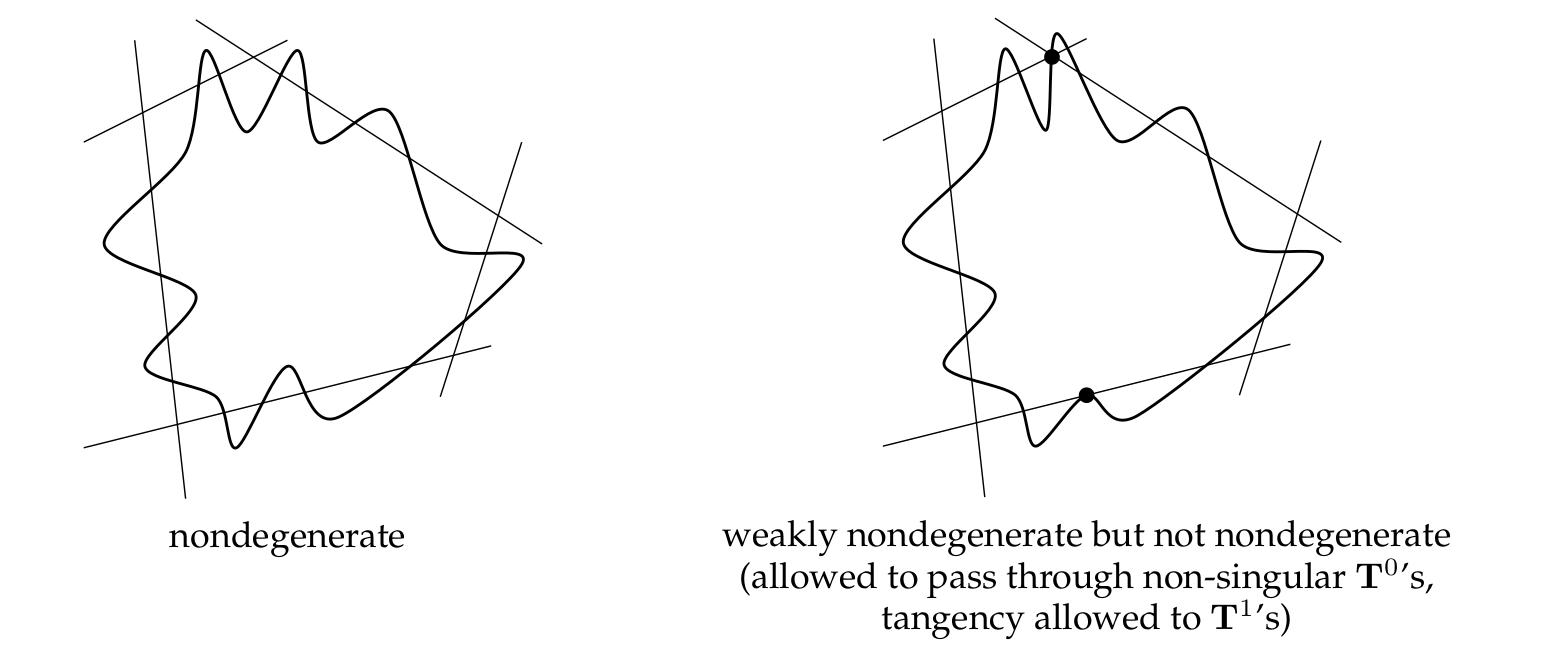
\includegraphics[width=\textwidth]{nondegeneracy}
\caption{The intersection properties of a curve with the toric divisor distinguishes nondegeneracy from weak nondegeneracy. Specifically for the curve to be nondegenerate, it must meet the toric divisor transversally and away from the codimension two $\Toric$-invariant divisors (Image credit \cite{WC_preface}).}
\end{figure}
\par
This condition on the nature of the intersection with the toric boundary is less intrinsic to the curve (for example, fixing a $\Gm{k}^2 \subset \P^2_k$ and a plane curve $C \subset \P^2_k$ we can always move the curve such that it intersects the three lines of the compliment of the torus transversally and does not pass through the intersection points of these three lines) and will often be inconsequential for results we would like to prove about such objects. Thus we define the weaker notion which ignores this intersection criterion.

\begin{defn}
We say that a Laurent polynomial $f \in k[x^{\pm 1}, y^{\pm 1}]$ is $\Delta$-\textit{toric} if $\Delta(f) \subset \Delta$ and $f$ defines a smooth curve $C_0 = U_f$ whose completion $C^\Delta_0 \embed \Toric_\Delta$ is smooth.
\end{defn}
\noindent
In the next section we will see how to reinterpret this condition purely in terms of properties of $f$, its Newton polygon, and the affine curve $U_f$.


\subsection{Baker's Theorem on the Genus for Toric Embeddings}

In this section, we discuss the classical result of Baker (1893) relating the genus of a smooth curve compactified in a toric surface to the enumerative properties of its associated convex lattice polygon.

\begin{thm}[Baker]
Let $f \in k[x^{\pm 1}, y^{\pm 1}]$ be a $\Delta$-nondegenerate Laurent polynomial. Then the toric completion $C_0^\Delta \embed \Toric_\Delta$ of $C_0 = U_f$ is a smooth Cartier divisor on $\Toric_\Delta$ and thus $C_0^\Delta$ is the unique smooth proper curve birational to $C_0$. Furthermore, the genus is computed via the number of interior lattice points of the Newton polygon, 
\[ g(C_0^\Delta) = |\Delta^\circ \cap \Z^2| \]
\end{thm}

\begin{proof}
Since $f$ is $\Delta$-nondegenerate, then $C_0^\Delta$ is an integral codimension one closed subscheme which does not intersect the singular locus of $\Toric_\Delta$ (in particular, if $x \in C_0^\Delta$ then $\stalk{\Toric_\Delta}{x}$ is a UFD) so $C_0^\Delta$ is Cartier. Since, by Lemma \ref{lemma_nondegeneracy}, the completion $C = C_0^\Delta$ is a smooth proper curve, its genus\footnote{If we assume $|\Delta^\circ \cap \Z^2| > 0$, then we do indeed have $H^0(C, \struct{C}) = k$ because the cokernel of $H^0(X, \struct{X}) \to H^0(C, \struct{C})$ is $H^1(X, \struct{X}(-D_C))$ which vanishes by the Batyrev-Borisov Vanishing theorem \cite[Thm. 9.2.7]{cox} because $\dim{\Delta} > 1$ and $D_C$ is ample. Regardless, we will find that $\dim_k H^0(C, \omega_C) = |\Delta^\circ \cap \Z^2|$ so $g(C) = |\Delta^\circ \cap \Z^2|$ in either case.} is $g(C) = \dim_k H^0(C, \Omega_{C/k})$ and $\Omega_{C/k} = \omega_{C}$ is its dualizing sheaf. Thus, we aim to compute $H^0(C, \Omega_C)$. Fixing notation, let $X = \Toric_\Delta$ and let $\iota : C \embed X$ be the inclusion. Choose a torus-invariant Cartier divisor $D_C$ linearly equivalent to the effective Cartier divisor $C$, in fact, we can explicitly write $D_C = C - \div{(f)}$ which is torus-invariant because it is supported on the toric divisor since $C|_{\Toric^n} = \div{(f)}|_{\Toric^n}$. We will now apply the adjunction exact sequence defined in Theorem \ref{adjunction},
\begin{center}
\begin{tikzcd}
0 \arrow[r] & \omega_X \arrow[r, "f"] & \omega_X(D_C) \arrow[r] & \iota_* \omega_C \arrow[r] & 0
\end{tikzcd}
\end{center}
Taking cohomology gives the following long exact sequence,
\begin{center}
\begin{tikzcd}
0 \arrow[r] & H^0(X, \omega_X) \arrow[r] & H^0(X, \struct{X}(D_C + K_X)) \arrow[r] & H^0(C, \omega_C) \arrow[r] & H^1(X, \omega_X)
\end{tikzcd}
\end{center} 
But $H^0(X, \omega_X) = H^0(X, \struct{X}(K_X)) = 0$ since the canonical divisor    has an empty corresponding polytope $P_{K_X} = \varnothing$. Furthermore, $H^1(X, \omega_X) = H^0(X, \struct{X}) = 0$ by Serre duality and Demazure vanishing. Therefore, the cohomology sequence gives an isomorphism,
\[ H^0(X, \struct{X}(D_C + K_X)) \xrightarrow{\sim} H^0(C, \omega_C) \]
In particular, the genus is,
\[ g(C) = \dim_k H^0(X, \struct{X}(D_C + K_X)) = | P_{D_C + K_X} \cap \Z^2 | \]
Thus, we need to compute $P_{D_C}$. Recall that under the embedding $\psi : \Toric_\Delta \embed \P^N_k$ the curve $C$ is the hyperplane section defined by the hyperplane,
\[ H_C = \sum_{(i, j) \in \Delta} a_{ij} X_{ij} \quad \text{ where } \quad f = \sum_{(i,j) \in \Delta} a_{ij} x^i y^j \]
Therefore, $\struct{X}(C) = \psi^* \struct{\P^N}(H_C) \cong \psi^* \struct{\P^N}(1)$ but recall that $\struct{X}(D_\Delta) = \psi^* \struct{\P^N}(1)$ so we find that $\struct{X}(C) \cong \struct{X}(D_\Delta)$. Therefore, $D_C \sim C \sim D_\Delta$ but both $D_C$ and $D_\Delta$ are torus-invariant so $P_{D_C} \cong_t \Delta$ (using that $P_{D_\Delta} = \Delta$). Decomposing,
\[ \Delta = \bigcap_{\substack{F \subset \Delta \\ \text{facet}}} H^+(n_F, - a_F) \]
we find,
\[ D_C \sim \sum_{\substack{F \subset \Delta \\ \text{facet}}} a_F D_F \]
Recall the canonical divisor is,
\[ K_X = - \sum_{\substack{F \subset \Delta \\ \text{facet}}} D_F \]
Thus,
\[ D_C + K_X \sim \sum_{\substack{F \subset \Delta \\ \text{facet}}} (a_F - 1) D_F \]
which implies that,
\[ P_{D_C + K_X} \cong_t \bigcap_{\substack{F \subset \Delta \\ \text{facet}}} H^+(n_F, 1 - a_F) = \Delta^{(1)} \]
since $\Delta$ is a lattice polygon. Therefore, we conclude,
\[ g(C) = | \Delta^{(1)} \cap \Z^2 | = | \Delta^\circ \cap \Z^2 | \]
\end{proof}

\begin{comment}

(RELATE THIS ABOVE FACT TO CANONICAL EMBEDDING)

\end{comment}

\begin{theorem} \label{adjunction}
Let $X$ be a normal projective Cohen-Macaulay variety, $\iota : C \embed X$ a prime divisor, and $D_C = C - \div{(f)}$ any linearly equivalent Weil divisor. Then there is an exact sequence,
\begin{center}
\begin{tikzcd}
0 \arrow[r] & \omega_X \arrow[r, "f"] & \omega_X(D_C) \arrow[r] & \iota_* \omega_C \arrow[r] & 0
\end{tikzcd}
\end{center}
\end{theorem}

\begin{rmk}
We will apply this theorem in the case when $D_C$ is chosen to be a $\Toric$-invariant Weil divisor but the proof does not depend on this fact.
\end{rmk}

\begin{proof}
The sheaf $\struct{X}(-D_C)$ is isomorphic to the sheaf of ideals defining $\iota : C \embed X$ giving an exact sequence,
\begin{center}
\begin{tikzcd}
0 \arrow[r] & \struct{X}(-D_C) \arrow[r, "f"] & \struct{X} \arrow[r] & \iota_* \struct{C} \arrow[r] & 0
\end{tikzcd}
\end{center}
Applying the functor $\shHom{\struct{X}}{-}{\omega_X}$ to the above short exact sequence gives a long exact sequence,
\begin{center}
\begin{tikzcd}
0 \arrow[r] & \shHom{\struct{X}}{\iota_* \struct{C}}{\omega_X} \arrow[r] \arrow[draw=none]{d}[name=Z, shape=coordinate]{} & \shHom{\struct{X}}{\struct{X}}{\omega_X} \arrow[r, "f"] & \shHom{\struct{X}}{\struct{X}(-D_C)}{\omega_X} 
\arrow[dll,
rounded corners, crossing over,
to path={ -- ([xshift=2ex]\tikztostart.east)
|- (Z) [near end]\tikztonodes
-| ([xshift=-2ex]\tikztotarget.west)
-- (\tikztotarget)}]
\\
& \shExt{1}{\struct{X}}{\iota_* \struct{C}}{\omega_X} \arrow[r] & \shExt{1}{\struct{X}}{\struct{X}}{\omega_X} \arrow[r] & \cdots
\end{tikzcd}
\end{center}
Since $\shHom{\struct{X}}{\struct{X}}{-}$ is the identity functor, $\shExt{1}{\struct{X}}{\struct{X}}{-} = 0$. Also, $\shHom{\struct{X}}{\iota_* \struct{C}}{\omega_X} = 0$ because $\iota_* \struct{C}$ is torsion but $\omega_X$ is torsion-free \cite[Ch. 1, Prop. 2.8]{grothendieck_duality}. Therefore, we find an exact sequence,
\begin{center}
\begin{tikzcd}
0 \arrow[r] & \omega_X \arrow[r, "f"] & \shHom{\struct{X}}{\struct{X}(-D_C)}{\omega_X} \arrow[r] & \shExt{1}{\struct{X}}{\iota_* \struct{C}}{\omega_X} \arrow[r] & 0
\end{tikzcd}
\end{center}
However, $X$ is Cohen-Macaulay (and projective) and $C$ is in codimension one so $\shExt{1}{\struct{X}}{\iota_* \struct{C}}{\omega_X}$ computes the dualizing sheaf $\iota_* \omega_C$ by \cite[Ch 1, Prop. 2.3]{grothendieck_duality}.
When $X$ is a normal projective variety, by Theorem \ref{canonical_reflexive}, the dualizing sheaf is reflexive with an associated canonical divisor Weil divisor $\omega_X = \struct{X}(K_X)$. Furthermore, by Theorem \ref{properties_of_reflexive_sheaves},
\[ \shHom{\struct{X}}{\struct{X}(-D_C)}{\omega_X} = \struct{X}(D_C + K_X) \]
Thus, we do get an exact sequence,
\begin{center}
\begin{tikzcd}
0 \arrow[r] & \struct{X}(K_X) \arrow[r, "f"] & \struct{X}(D_C + K_C) \arrow[r] & \iota_* \omega_C \arrow[r] & 0
\end{tikzcd}
\end{center}
viewing $f$ as a section of $\struct{X}(D_C)$, using that $D_C + \div{(f)} = C$ is effective, gives $\struct{X} \xrightarrow{f} \struct{X}(D_C)$. Then, tensoring by $- \otimes_{\struct{X}} \omega_X$ and using $\struct{X}(D) \otimes_{\struct{X}} \struct{X}(E) \to \struct{X}(D + E)$ via $f \otimes g \mapsto fg$ gives the above map.
\end{proof}

\noindent
The previous theorem shows that $\Delta$-nondegeneracy is sufficient for the closure of $U_f$ to embed smoothly. However, it is not necessary since the condition requires that the curve does not pass through the codimension-two toric components. We will use the following remark to weaken our nondegeneracy condition on $f$. First, we prove an extension of Baker's theorem which applies without the nondegeneracy condition.

\begin{thm} \label{baker_refinement}
For \textit{any} Laurent polynomial $f \in k[x^{\pm 1}, y^{\pm 1}]$ such that $U_f$ is a curve and $\Delta(f) = \Delta$,
\[ g(U_f) \le | \Delta^\circ \cap \Z^2 | \]
with equality exactly when the scheme theoretic image of $U_f \embed \Toric_\Delta$ is smooth. 
\end{thm}

\begin{proof}
See \cite[Section 2]{tim} and \cite[Section 2]{WC_zeta_functions}. Here, we will give a sketch of the proof. Let $V \subset \Delta$ be the vertices and $S = (\Delta \cap \Z^2) \setminus V$ the non vertex lattice points. Then, the parameter space of Laurent polynomials $f \in k[x^{\pm 1}, y^{\pm 1}]$ such that $\Delta(f) = \Delta$ is exactly $L = \A_k^{S} \times_k \Gm{k}^V$ with coordinates $x_{ij}$ for $(i,j) \in \Delta$, where we associate a $k$-rational point $(a_{ij}) \in \A_k^{S} \times_k \Gm{k}^V$ to the Laurent polynomial,
\[ f = \sum_{(i,j) \in \Delta} a_{ij} x^i y^j \]
Note that $\Delta(f) = \Delta$ since the coefficients $a_{ij}$ corresponding to vertices $(i,j) \in \Delta$ are nonzero.
Now, consider the closed subscheme,
\[ V \subset \Gm{k}^2 \times_k \A_k^{S} \times_k \Gm{k}^{V} = \Spec{k[x^{\pm 1}, y^{\pm 1}]} \times \Spec{k[(a_{ij})_{(i, j) \in S}, (a_{i,j}^{-1})_{(i,j) \in V}]} \]
defined by the vanishing,
\[ V = V\left( \sum_{(i,j) \in \Delta} a_{ij} x^i y^j \right) \]
Then the projection gives a family $\pi : V \to L$ of torus curves parameterized by the coefficients of their Laurent polynomials. Now, we complete $V$ under the open immersion $\Gm{k}^2 \times_k L \embed \Toric_\Delta \times_k L$ to get a closed immersion $\C \embed \Toric_\Delta \times_k L$ whose fiber over $f$ gives the $\Delta$-toric completion of $U_f$, 
\begin{center}
\begin{tikzcd}[row sep = huge]
V \arrow[r, hook] \arrow[drr] & \C \arrow[r, hook] \arrow[dr] & \Toric_\Delta \times_k L \arrow[d, "\pi"]
\\
& & L
\end{tikzcd}
\end{center}
By \cite[Section 2, Prop. 1]{WC_zeta_functions}, the locus of $L$ corresponding to $\Delta$-nondegenerate $f$ contains a Zariski dense open. Therefore, the general fiber $\mathcal{C}_{f_0}$ above $f_0 \in k[x^{\pm 1}, y^{\pm 1}]$ corresponds to $C_0^\Delta$, the completion of $C_0 = U_{f_0}$, which is smooth proper curve with genus and thus arithmetic genus,
\[ g_a(U_f^\Delta) = g(U_f^\Delta) = | \Delta^\circ \cap \Z^2 | \]
by the version of Baker's theorem proven above.
\bigskip\\
I claim the family $\C \to L$ is flat. First, the projection $X = \Toric_{\Delta} \times_k L \to L$ is flat meaning that $\stalk{L}{\pi(x)} \to \stalk{X}{x}$ makes $\stalk{X}{x}$ a flat $\stalk{L}{\pi(x)}$-module. The Laurent polynomial $f$ is a section of the line bundle $\struct{\Toric_\Delta}(D_\Delta) \boxtimes \struct{L}$ which is generated by the global sections $x^i y^j$ for $(i,j) \in V$ by Lemma \ref{polytope_div_ample}. Furthermore, coefficient functions $a_{ij} \in \Gamma(L, \struct{L})$ with $(i,j) \in V$ are non-vanishing. Since it suffices to check flatness on closed points, take any closed point $x \in \Toric_\Delta \times_k L$, then the germ $f \in \stalk{X}{x} / \m_{\pi{x}} \stalk{X}{x} = \stalk{X}{x}\otimes_{\stalk{L}{\pi(x)}} \kappa(\pi(x))$ is a zero divisor exactly when $f$ is the zero polynomial after evaluating the coefficients at $\pi(x) \in L$. However, all the $a_{ij}$ with $(i, j) \in V$ are non-vanishing on $L$ so $f \in \stalk{X}{x} / \m_{\pi{x}} \stalk{X}{x}$ is never the zero polynomial. Then applying \cite[\href{https://stacks.math.columbia.edu/tag/046Z}{Tag 046Z}]{stacks-project} we see that $\stalk{L}{\pi(x)} \to \stalk{X}{x}/(f)$ is flat and thus $\C \to L$ is flat.
\bigskip\\
Furthermore, $\C \embed \Toric_\Delta \times_k L\embed \P^n_k \times_k L$ is a closed subscheme so applying \cite[Thm. III.9.10]{har}, the arithmetic genus of the fibers is constant. Thus, for any $f \in k[x^{\pm 1}, y^{\pm 1}]$ such that $U_f$ is a smooth curve, then its toric completion $U_f^\Delta$ has arithmetic genus,
\[ g_a(U_f^\Delta) = g_a(C_0^\Delta) = | \Delta^\circ \cap \Z^2 | \]
We use Lemma \ref{genus_formulas} to conclude that,
\[ g(U_f) = g(U_f^\Delta) \le g_a(U_f^\Delta) = | \Delta^\circ \cap \Z^2 | \]
and an equality exactly when $U_f^\Delta$ is smooth. Furthermore, since $\C \to L$ is a proper flat family, by Zariski connectedness the fibers are connected so we see that \textit{any} $U_f^\Delta$ with $\Delta(f) = \Delta$ is connected (even when $U_f$ is not a curve, e.g. $U_f$ not connected).
\end{proof}

\begin{rmk}
We have shown that $U_f^\Delta$ is connected whenever $\Delta(f) = \Delta$ but the affine scheme $U_f$ certainly may not be. For example, consider $f_1 = (x + y - 1)(x + y + 1)$ and $f_2 = x^2 + y^2 - 1$ then $\Delta(f_1) = \Delta(f_2) = 2 \Sigma$ where $\Sigma$ is the unit isosceles right triangle. However, 
\[ U_{f_1} = \Spec{k[x^{\pm 1}, y^{\pm 1}]/(f_1)} = \Spec{k[k[x^{\pm 1}, y^{\pm 1}]/(x + y - 1)} \times_k \Spec{k[k[x^{\pm 1}, y^{\pm 1}]/(x + y + 1)} \]
which is the union of two parallel lines in $\Gm{k}^2$ (which do not intersect in the torus) while,
\[ U_{f_2} = \Spec{k[x^{\pm 1}, y^{\pm 1}]/(f_2)} = \Spec{k[x^{\pm 1}, y^{\pm 1}]/(x^2 + y^2 - 1)} \]
is irreducible and thus connected. However, in the toric completion $U_{f_1}^\Delta$ (which lies in $\Toric_{2 \Sigma} = \P^2_k$), these two parallel lines do in fact intersect so both $U_{f_1}^\Delta$ and $U_{f_2}^\Delta$ are connected.
\end{rmk}


\begin{defn} \label{weakly_defn}
We say that $f \in k[x^{\pm 1}, y^{\pm 1}]$ is \textit{weakly} $\Delta$-\textit{nondegenerate} when the following hold,
\begin{enumerate}
\item $\Delta(f) \subset \Delta$
\item for each face $\tau \subset \Delta$ we have $\tau \cap \Delta(f) \neq \empty$
\item the affine curve $U_f$ is smooth with genus $g(U_f) = | \Delta^{(1)} \cap \Z^2 |$. 
\end{enumerate}
\end{defn}
\noindent
Weakly $\Delta$-nondegenerate Laurent polynomials $f \in k[x^{\pm 1}, y^{\pm 1}]$ do indeed define affine curves $U_f$ with an embedding $U_f \embed \Toric_\Delta$ such that the completion $C_0^\Delta$ is smooth and satisfies the numerical genus condition of Baker. However, such curves will not, in general, be Cartier divisors on $\Toric_\Delta$ since they may pass through the singular locus where $\Toric_\Sigma$ is not locally factorial. 

\begin{lemma}
Assuming parts (a) and (b) of Definition \ref{weakly_defn}, part (c) is equivalent to the condition that the scheme-theoretic image of $U_f \embed \Toric_\Delta$ is smooth. 
\end{lemma}

\begin{proof}
When $U_f^\Delta$ is smooth, $g(U_f^\Delta) = g_a(U_f^\Delta) = | \Delta^\circ \cap \Z^2|$. Conversely, we have that $\tilde{\Delta} = \Delta(f) \subset \Delta$ (from the definition that $f$ is weakly $\Delta$-nondegenerate) and we assume $g(U_f) = | \Delta^\circ \cap \Z^2 |$. From Baker's bound,
\[ g(U_f^\Delta) = g(U_f) \le |\tilde{\Delta}^\circ \cap \Z^2| \le |\tilde{\Delta}^\circ \cap \Z^2 | \] 
Thus, from the assumption these are equalities so,
\[ g(U_f^\Delta) = | \tilde{\Delta}^\circ \cap \Z^2 | \]
and thus $U_f^\Delta$ is smooth by the above result.
\end{proof}

\begin{comment}

\subsection{Combinatorial Gonality (WIP)}

\begin{defn}
Let $C$ be a curve over $k$. The \textit{gonality} $\gon{C}$ is defined to be the minimal degree of a non-constant morphism $C \to \P^1_k$. 
\end{defn}

\end{comment} 

\subsection{The Inverse Situation}

Up until now we have discussed the situation of specifying a curve by a fixed Laurent polynomial and attempting to describe the unique smooth complete curve in its birationality class via a toric completion. Here we consider the inverse problem: given a (smooth complete) curve $C$, we might ask when one can find a dense open set $U \subset C$ with a closed embedding $U \embed \Gm{k}^2$ such that the resultant Laurent polynomial describing the torus curve $U$ satisfies the nondegeneracy conditions we have discussed earlier. 

\begin{defn}
Given a convex lattice polygon $\Delta$, we say that a curve $C$ over $k$ is \textit{(weakly)} $\Delta$-\textit{nondegenerate} over $k$ if it is birational over $k$ to a curve $U \subset \Toric^2$ such that $U = V(f)$ for some (weakly) $\Delta$-nondegenerate Laurent polynomial $f \in k[x^{\pm 1}, y^{\pm 1}]$. In the case that $C$ is weakly $\Delta$-nondegenerate, we will alternatively say that $C$ is $\Delta$-toric to emphasize that $C$ embeds into the toric surface $\Toric_\Delta$. Furthermore, we say that $C$ is \textit{geometrically (weakly)} $\Delta$-\textit{nondegenerate} if $C \times_k \bar{k}$ is (weakly) $\Delta$-nondegenerate over $\bar{k}$.  
\end{defn}
\noindent\\
First we note that using the terms weakly $\Delta$-nondegenerate and $\Delta$-toric interchangeably will introduce no confusion because of the following result which shows that any curve which may be embedded in a toric surface is weakly nondegenerate.

\begin{prop}
Let $C \embed \Toric_\Delta$ be an embedding of a non-rational smooth curve into a toric surface. Then $C$ is weakly $\tilde{\Delta}_C$-nondegenerate where $\tilde{\Delta}_C = \Conv{P_C \cap \Z^2}$. 
\end{prop}

\begin{proof}
Since $C$ is nonrational, it cannot lie in the toric divisor $D_\Toric$ which is a union of toric varieties which are rational because every irreducible subvariety of the toric divisor is rational. Therefore it must intersect the torus, $C \cap \Toric^2 \neq \varnothing$ so $C \cap \Toric^2$ gives some curve $U_f \subset \Gm{k}^2$ defined by an irreducible Laurent polynomial $f \in k[x^{\pm 1}, y^{\pm 1}]$. Then the linearly equivalent divisor $D_C = C - \div{(f)}$ is torus-invariant since it is supported on $D_\Toric$ because $C |_{\Toric^2} = \div{(f)} |_{\Toric^2}$ on the torus. 
\bigskip\\
Now we consider the rational polytope $P_{D_C}$ of the torus-invariant Weil divisor $D_C$ (note $D_C$ may not be Cartier and $P_{D_C}$ may not be a lattice polytope). However, $D_C + \div{(f)} = C$ is effective so $f \in H^0(\Toric_\Delta, \struct{\Toric_\Delta}(D_C))$ which implies that $\Delta(f) \subset P_{D_C}$ because there is a decomposition,
\[ H^0(\Toric_\Delta, \struct{\Toric_\Delta}(D_C)) = \bigoplus_{(i,j) \in P_{D_C} \cap \Z^2} k \cdot x^i y^j \]
so the support of $f$ must be contained in $P_{D_C} \cap \Z^2$. Even better, this shows that,
\[ \Delta(f) \subset \Conv{P_{D_C} \cap \Z^2} = \tilde{\Delta}_C \subset P_{D_C} \]
Now, since $C$ is smooth, by our refinement of Baker's bound (Theorem \ref{baker_refinement}) we have,
\[ g(C) \le |\Delta(f)^{(1)} \cap \Z^2| \le |\tilde{\Delta}_C^{(1)} \cap \Z^2 | \]
As in the proof of Baker's theorem, we want to apply the exact sequence of Theorem \ref{adjunction},
\begin{center}
\begin{tikzcd}
0 \arrow[r] & \struct{X}(K_X) \arrow[r] & \struct{X}(D_C + K_X) \arrow[r] & \struct{C}(K_C) \arrow[r] & 0
\end{tikzcd}
\end{center}
which gives an isomorphism $H^0(X, \struct{X}(D_C + K_X)) \xrightarrow{\sim} H^0(C, \omega_C)$. 
\end{proof}

\begin{rmk}
Notice, in the proof of Theorem \ref{baker_refinement}, we use the fact (proven in \cite[Section 2, Prop. 1]{WC_zeta_functions}) that the generic Laurent polynomial $f \in k[x^{\pm 1}, y^{\pm 1}]$ with fixed Newton polygon $\Delta$ is $\Delta$-nondegenerate. However, we have shown that a very general curve cannot lie on any toric surface and thus cannot be $\Delta$-toric let alone $\Delta$-nondegenerate. How can these facts be consistent? It must be that under the equivalence relation,
\[ f \sim f' \iff U_f \birat U_{f'} \iff \Frac{k[x^{\pm 1},y^{\pm 1}]/(f)} \cong \Frac{k[x^{\pm 1},y^{\pm 1}] / (f')} \]
a general equation does not define a class corresponding to a general curve. In fact, the general Laurent polynomial $f \in k[x^{\pm 1}, y^{\pm 1}]$ with fixed $\Delta = \Delta(f)$ lies in the subspace of the moduli space corresponding to $\Delta$-nondegenerate curves.
\end{rmk}

Since the two notions are very similar, we naturally ask if weak and strong $\Delta$-regularity are equivalent properties. Restricting to a fixed lattice polygon $\Delta$, Castryck has provided a negative answer to this question by constructing a weakly $\Delta$-nondegenerate curve with no embedding into $\Toric_\Delta$ which intersects the toric divisor transversally. In particular, he showed the following.

\begin{prop} \label{example_weak_only}
There exists a lattice polygon $\Delta$ and a curve $C$ such that $C$ is weakly $\Delta$-nondegenerate but not $\Delta$-nondegenerate. Specifically, consider the Laurent polynomial,
\[ f = x^5 + y^2 + x^2 y^3 + 1 \in k[x^{\pm 1}, y^{\pm 1}] \]
and the lattice polygon $\Delta = \Conv{\{ (0,0), (5, 0), (2, 3), (0,3) \}}$.
\begin{figure}
\begin{center}
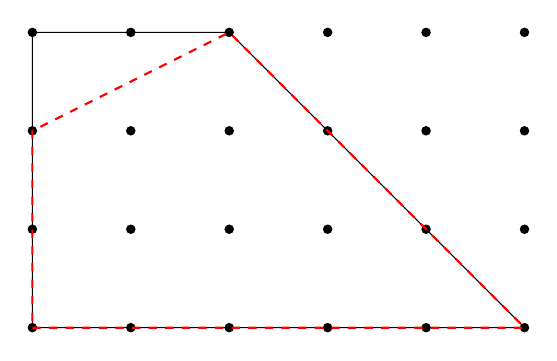
\begin{tikzpicture}

\foreach \x in {0,1,2,3,4,5}
   \foreach \y in {0,1,2,3} 
      \draw[fill] (5/4*\x,5/4*\y) circle (1.5pt) coordinate (m-\x-\y);

% using named coordinates
\draw (m-0-0) -- (m-5-0) -- (m-2-3) -- (m-0-3) -- cycle;
\draw[red, dashed, thick] (m-0-0) -- (m-5-0) -- (m-2-3) -- (m-0-2) -- cycle;
\end{tikzpicture}
\end{center}
\caption{The polygons $\Delta$ in black and $\Delta(f)$ in red for $f = x^5 + y^2 + x^2 y^3 + 1$ in example of Proposition \ref{example_weak_only}.}
\end{figure}
\end{prop}

\begin{proof}
See \cite[Lemma 4.4]{WC_linear_pencils}. The proof uses the theory of trigonal curves and the canonical embedding. Furthermore, for this particular choice of polygons, $\Delta^{(1)}$ and $\Delta$ have the same normal fan so we can identify the toric compactification of this curve with its canonical image. We can understand intuitively why this example works. The toric variety $\Toric_{\Delta}$ is a Hirzebruch surface and the curve $C_0^\Delta \embed \Toric_{\Delta}$ is tangent to the torus divisor at the component defined by the vertex $V = (0,3)$ in the polygon $\Delta$ showing that this curve is not $\Delta$-nondegenerate. Furthermore, the Hirzebruch surface has a single-parameter family of automorphism which translates the tangency point along the toric divisor. Thus no modification of $C_0$ can be $\Delta$-nondegenerate. Notice that $\Delta(f) \subsetneq \Delta$ and the normal fan of $\Delta(f)$ contains an additional ray. Therefore, $\Toric_{\Delta(f)}$ corresponds to the toric blowup of the tangency point which turns the tangency into a transverse intersection which explains why $f$ is $\Delta(f)$-nondegenerate although it is not $\Delta$-nondegenerate.
\end{proof}

\begin{figure}
\begin{center}
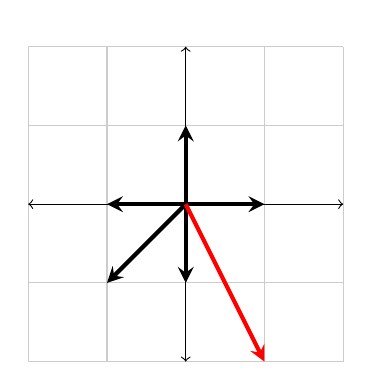
\begin{tikzpicture}
  \draw[thin,gray!40] (-2,-2) grid (2,2);
  \draw[<->] (-2,0)--(2,0) node[right]{};
  \draw[<->] (0,-2)--(0,2) node[above]{};
  \draw[line width=1.5pt,-stealth](0,0)--(-1,-1) node[anchor=south west]{$ $};
  \draw[line width=1.5pt,-stealth](0,0)--(-1,0) node[anchor=south west]{$ $};
  \draw[line width=1.5pt,-stealth](0,0)--(0,-1) node[anchor=south west]{$ $};
  \draw[line width=1.5pt,-stealth](0,0)--(0,1) node[anchor=north east]{$ $};
  \draw[line width=1.5pt,-stealth](0,0)--(1,0) node[anchor=south west]{$ $};
  \draw[line width=1.5pt,red,-stealth](0,0)--(1,-2) node[anchor=south west]{$ $};
\end{tikzpicture}
\end{center}
\caption{Rays of the normal fans of $\Delta$ (black) and $\Delta(f)$ (red). Notice that the normal fan of $\Delta(f)$ gives a toric blowup of the fan of $\Delta$.}
\end{figure}
\noindent
Notice that the curve Castryck constructs is actually nondegenerate (with respect to its own Newton polygon) and is only not nondegenerate for a specific choice of $\Delta$ for which it is weakly $\Delta$-nondegenerate. We suspect that there exist examples of curves which are $\Delta$-toric for some $\Delta$ but never $\Delta$-nondegenerate \textit{for any} $\Delta$. However, as of now, such examples remain elusive. Although we have shown that a very general curve cannot be $\Delta$-toric (let alone $\Delta$-nondegenerate) for any $\Delta$, low genus curves turn out to be well-behaved with respect to toric regularity. In particular, Castryck showed that all curves of genus $4$ or less admit a nondegenerate affine equation.


\begin{thm}[Cas17, Thm. 10]
Every curve $C / k$ of genus $g(C) \le 4$ is $\Delta$-nondegenerate for exactly one of a fixed finite list of lattice polygons.
\end{thm}


\begin{comment}


\subsection{Can We Give Example Never $\Delta$-nondegenerate (WIP)}


\subsection{Moduli Problem for Nondegenerate Curves (WIP)}


\subsection{Curves in Hirzebruch Surfaces (WIP)}

\end{comment}

\newcommand{\X}{\mathcal{X}}

\section{Models of Curves}

Here we discuss the general theory of models over discrete valuation rings (DVRs) which is the necessary theory for reduction of curves. Standard references for this topic are \cite[\href{https://stacks.math.columbia.edu/tag/0C2R}{Tag 0C2R}]{stacks-project} which discusses models in the context of semistable reduction and \cite[Chapter 9]{liu} who studies the more general problem of regular and minimal fibered surfaces over Dedekind schemes. We will not provide detailed proofs as doing so would require getting too much into the weeds of fibered surfaces but we will make care to lay out the definitions and properties in the necessary detail.

\begin{rmk}
We will be in the situation where $R$ is a DVR and $K = \Frac{R}$ its fraction field. Then let $\m \subset R$ be the maximal ideal and $\kappa = R / \m$ the residue field. We may distinguish the \textit{geometric} case in the special fiber when $\kappa$ is algebraically closed and otherwise when $\kappa$ admits algebraic extensions. 
\end{rmk}

\begin{defn}
Let $C$ be a scheme of finite type over $K$. A \text{model} $X \to \Spec{R}$, of $C$ over $R$, consists of scheme $X$ flat and proper over $R$ with a given isomorphism $C \xrightarrow{\sim} X_K$ where $X_K = X \times_{\Spec{R}} \Spec{K}$ is the generic fiber. A morphism $f : X \to X'$ of models of $C$ is an $R$-morphisms of schemes inducing an isomorphism $f : X_K \xrightarrow{\sim} X'_K$ compatible with the isomorphisms $C \xrightarrow{\sim} X_K$ and $C \xrightarrow{\sim} X_K'$.
\end{defn}

\begin{rmk}
We require models to be flat over $R$ so that the generic fiber $X_K$ and the special fiber $X_\kappa = X \times_{\Spec{R}} \Spec{\kappa}$ form a flat family over $\Spec{R}$ such that numerical invariants are preserved under the degeneration from the general to the special fiber. Note, we further require models to be proper unlike the definition in \cite[\href{https://stacks.math.columbia.edu/tag/0C2R}{Tag 0C2R}]{stacks-project}. We will emphasize the definition whenever it becomes likely to cause confusion.
\end{rmk}

\begin{rmk}
Our main reference \cite[Chapter 9]{liu} defines models not for curves over $K$ rather for fibered surfaces over a Dedekind scheme, e.g. $\Spec{R}$ in which a model of $X \to S$ is defined as a fibered surface $X'$ with a birational map $X' \rat X$. Notice, however, any two models $X, X'$ of $C$ are automatically birational since the map $X_K \iso C \iso X'$ is an isomorphism of dense open sets ($\Spec{K} \embed \Spec{R}$ is an open immersion when $R$ is a DVR so its base change to $X_K \embed X$ is an open immersion as well) giving a birational map $X \rat X'$. Therefore, $X$ and $X'$ are models of each other in the sense of Liu allowing a direct carrying over of the results. 
\end{rmk}

\begin{prop} \label{resolution_of_models}
Let $C$ be a smooth projective curve over $K$ and $X$ a model of $C$ over $R$. Then $X$ admits a resolution of singularities $\tilde{X} \to \Spec{R}$ and any such resolution is a model of $C$.
\end{prop}

\begin{proof}
This result follows from the general criteria for resolution of surfaces due to Lipman \cite{Lipman}. See \cite[\href{https://stacks.math.columbia.edu/tag/0C2U}{Tag 0C2U}]{stacks-project} for details.
\end{proof}

\subsection{Minimal Models} 


\renewcommand{\N}{\mathcal{N}}

\begin{defn}
Let $C$ be a smooth projective curve over $K$ with $H^0(C, \struct{C}) = K$. A \textit{minimal model} of $X$ is a regular (proper) model $X \to \Spec{R}$ of $C$ such that for any other regular (proper) model $X' \to \Spec{R}$ there is a unique morphism of models $X' \to X$ i.e. a morphism $X' \to X$ making the diagram commute,
\begin{center}
\begin{tikzcd}[column sep = small]
X' \arrow[rr, dashed] & & X
\\
X'_K \arrow[u, hook] \arrow[rr, equals] & & X_K \arrow[u, hook] 
\\
& C \arrow[ru, equals] \arrow[lu, equals]
\end{tikzcd}
\end{center}
\end{defn}

\begin{lemma}
If it exists, a minimal model of $C$ is unique.
\end{lemma}

\begin{proof}
This follows directly from the definition. If $X$ and $X'$ are two minimal models of $C$ then we get birational morphisms $X \to X'$ and $X' \to X$. Even better, they compose to the unique morphism of models $X \to X$ and $X' \to X'$ which must be the identities.
\end{proof}

\begin{rmk}
Uniqueness of the morphism of models $X' \to X$ is automatic since it is required, on the generic fiber, to be the unique isomorphism determined by the identification of the generic fibers with $C$. Since the generic fiber is dense and these are reduced separated schemes there is a unique morphism $X' \to X$ extending this isomorphism. In fact, this argument shows a more general fact.
\end{rmk}

\begin{lemma} \label{existence_inverses}
Between any two models $X, X'$ of $C$ there is a birational map $X \rat X'$. If there exists a morphism of models $X \to X'$ it is unique. In particular, if there exist morphisms $X \to X'$ and $X' \to X$ then they are inverses so $X \cong X'$. 
\end{lemma}
\noindent
We can convert the fairly abstract notion of minimality into a concrete condition on sorts of exceptional curves which do not occur as divisors. In particular, a minimal model will turn out to be a model which does not contain any exceptional curves which may be blown down while retaining the regularity of the surface.

\begin{definition}
We call the following an \textit{exceptional curve of the first kind}:
\bigskip\\
Let $X$ be a Noetherian scheme. Let $E \subset X$ be a closed subscheme with the following properties,
\begin{enumerate}
\item $E$ is an effective Cartier divisor on $X$,
\item there exists a field $k$ and an isomorphism $\P^1_k \to E$,
\item the normal sheaf $\mathcal{N}_{E/X}$ pulls back to $\struct{\P^1_k}(-1)$. 
\end{enumerate}
\end{definition}

\begin{rmk}
In the case that $X \to \Spec{k}$ is a surface over a field $k$. We can reinterpret the condition of the normal bundle $\N_{E/X}$ that it pullback to $\struct{\P^1_k}(-1)$ in terms of intersection theory. Recall that given dimension one cycles $C_1, C_2 \subset X$ we can define the intersection number,
\[ C_1 \cdot C_2 = \chi(\struct{X}(C_1)|_{C_2}) - \chi(\struct{C_2}) \]
In general, there is an intersection product on the Chow groups $\CH^i(X) \times \CH^j(X) \to \CH^{i+j}(X)$ giving $\CH^\bullet(X)$ a ring structure defining the Chow ring. In our case the intersection number is the map,
\[ \CH^{1}(X) \times \CH^{1}(X) \to \CH^2(X) \xrightarrow{\deg} \Z \]
where the degree map $\deg : \CH^2(X) \to \Z$ exists on a proper surface $X$ since relations in $\CH^2(X)$ are given by divisors of functions on closed curves in $X$ which have zero degree on proper curves. This agrees with the intersection number $C_1 \cdot C_2 = \chi(\struct{X}(C_1)|_{C_2}) - \chi(\struct{C_2})$. Now, consider the self-intersection $C \cdot C = \chi(\struct{X}(C)|_C) - \chi(\struct{C})$. However, since $\struct{X}(C)$ is the dual of the sheaf of ideals defining $\iota : C \embed X$ then $\struct{X}(C)|_C = (\iota^* \I)^\vee = \N_{C/X}$ is the normal bundle. Therefore, $C \cdot C = \chi(\N_{C/X}) - \chi(\struct{C})$ for a Cartier divisor $C \embed X$. In the case that $C$ is a smooth curve on a projective surface, we have using Riemann-Roch,
\[ C \cdot C = \chi(\N_{C/X}) - \chi(\struct{C}) = \deg{(\N_{C/X})} \]
When $E$ is an exceptional curve with an isomorphism $f : \P^1_k \xrightarrow{\sim} E$ such that $f^* \N_{E/X} = \struct{\P^1_k}(-d)$ then $E \cdot E = \deg{(\N_{E/X})} = \deg{\struct{\P^1_k}(-d)} = -d$. We say in this case that $E$ is a $(-d)$-curve. 
\bigskip\\
The astute reader may notice that the arithmetic surfaces we wish to study are not defined over a field. However, if $C_1, C_2 \subset X$ are Cartier divisors contained the in special fiber $X_\kappa$, in particular if $C_1, C_2$ are irreducible components of $X_\kappa$, then we may salvage the above discussion. Such divisors above the residue field $k$ are sometimes in the literature (e.g. \cite{romagny_models}) called \textit{vertical divisors} to distinguish them from \textit{horizontal divisors} which are finite flat over $\Spec{R}$. Since $C_1, C_2$ are curves over $\kappa$ and thus the degree of the intersection, $(C_1 \cdot C_2) = \deg{(C_1 \cap C_2)}$ in $\CH^2(X)$ may be computed via degree and Euler characteristic as above. This intersection form is developed in detail in \cite[\href{https://stacks.math.columbia.edu/tag/0C5Y}{Tag 0C5Y}]{stacks-project}.
\end{rmk}
\noindent
Following the conventions of Liu, we say that a model not containing any exceptional curves of the first kind is a relatively minimal model. We remark that this is the definition of a \textit{minimal model} given in \cite[\href{https://stacks.math.columbia.edu/tag/0C2R}{Tag 0C2R}]{stacks-project}. In the next section, we will see why this definition makes sense and coincides with ours in the case of positive genus curves.

\begin{definition}
Let $C$ be a smooth projective curve over $K$ with $H^0(C, \struct{C}) = K$. A \textit{relatively minimal model} is a regular, proper model $X$ of $C$ such that $X$ does not contain an exceptional curve of the first kind. 
\end{definition}

\subsection{Contracting Exceptional Curves}

\begin{defn}
Let $f : X \to Y$ be a morphism of schemes and $E \subset X$ an effective Cartier divisor. Then $f : X \to Y$ is a \textit{contraction of} $E$ if $f$ is proper such that $f(E) = \{ y \}$ for some closed point $y \in Y$ where $\stalk{Y}{y}$ is regular and $\dim{\stalk{Y}{y}} = 2$ and such that $f : X \to Y$ is the blowup of $Y$ with center at the closed point $y$.
\end{defn}

\begin{rmk}
Note that since $f : X \to Y$ is a blowup, it is a birational morphism giving an isomorphism $X \setminus E \iso Y \setminus \{ y \}$. Therefore, if $X$ is regular then $Y$ is regular automatically at every point except possibly $y \in Y$ which is assumed to be regular as part of the definition. Therefore, we see that contraction preserves regularity.
\end{rmk}

\begin{lemma}[0C5J]
Let $X$ be a Noetherian scheme. Let $E \subset X$ be an exceptional curve of the first kind. If a contraction $f : X \to Y$ of $E$ exists, then it satisfies the following universal property: every morphism $\varphi : X \to Z$ such that $\varphi(E)$ is a point, then $\varphi$ factors uniquely through $f : X \to Y$,
\begin{center}
\begin{tikzcd}[column sep = small, row sep = large]
E \arrow[r, hook] \arrow[d, "f"'] & X \arrow[r, "\varphi"] \arrow[d, "f"'] & Z
\\
\Spec{\kappa(x')} \arrow[r, hook] & Y \arrow[ru, dashed, "\tilde{\varphi}"']  
\end{tikzcd}
\end{center}
\end{lemma}

\begin{corollary}
If it exists, any contraction of $E \subset X$ is unique up to unique isomorphism. 
\end{corollary}

\begin{proof}
Uniqueness following directly from the universal property.
\end{proof}


\begin{prop}[\href{https://stacks.math.columbia.edu/tag/0C5L}{Tag 0C5L}] \label{picard_blowdown}
Let $b : X \to X'$ be a contraction on an exceptional curve of the first kind $E \embed X$. Then the morphisms $E \embed X \to X'$ induce a short exact sequence,
\begin{center}
\begin{tikzcd}
0 \arrow[r] & \Pic{X'} \arrow[r] & \Pic{X} \arrow[r] & \Pic{E} \arrow[r] & 0
\end{tikzcd}
\end{center}
Furthermore, since $E \cong \P^1_k$ we have $\Pic{E} \cong E$ and the map $\Pic{E} \to \Pic{X}$ via $n \mapsto \struct{X}(-n E)$ makes the above sequence split. 
\end{prop}

\begin{prop}[\href{https://stacks.math.columbia.edu/tag/0C2M}{Tag 0C2M}] \label{existence_of_blowdown}
Let $X \to S$ be proper over an affine Noetherian scheme $S$. Let $\L$ be an ample invertible $\struct{X}$-module and $E \subset X$ an exceptional curve of the first kind. Then there exists a contraction $b : X \to X'$ of $E$ such that $X' \to S$ is proper and $\L$ induces an invertible $\struct{X'}$-module $\L'$ via Lemma \ref{picard_blowdown}. 
\end{prop}


\subsection{Existence of Minimal Models}

From now on in our discussion of models, let $C$ be a fixed smooth projective curve over $K$ with $H^0(C, \struct{C}) = K$. We will consider the existence of various models of $C$ over $R$. 

\begin{lemma} \label{blow_down_chains}
Let $X$ is a regular (proper) model of $C$ over $R$, then there exists a sequence of morphisms,
\begin{center}
\begin{tikzcd}
X = X_m \arrow[r] & X_{m-1} \arrow[r] & \cdots \arrow[r] & X_1 \arrow[r] & X_0
\end{tikzcd}
\end{center}
of proper regular models of $C$, such that each morphism is a contraction of an exceptional curve of the first kind, and such that $X_0$ is a relatively minimal model.
\end{lemma}

\begin{proof}
This follows via a repeated application of Lemma \ref{existence_of_blowdown} until $X_0$ contains no further exceptional curves of the first kind since such contractions preserve properness, regularity, and the existence of an ample line bundle. Thus, it suffices to show that $X$ has an ample line bundle but $X$ is quasi-projective by \cite[\href{https://stacks.math.columbia.edu/tag/0C5N}{Tag 0C5N}]{stacks-project} so this is immediate from an immersion into projective space.
\end{proof}


\begin{proposition}
A relatively minimal model of $C$ over $R$ exists.
\end{proposition}

\begin{proof}
Choose a closed immersion $C \embed \P^n_K$ and let $X$ be the scheme-theoretic image of the immersion, $C \embed \P^n_K \embed \P^n_R$. Then $X \to \Spec{R}$ is a projective model of $C$ and there exists a resolution of singularities $\tilde{X} \to X$ and $\tilde{X}$ is a model for $C$ (Lemma \ref{resolution_of_models}). Then $\tilde{X} \to \Spec{R}$ is proper as a composition of proper morphisms. Then we use the previous result to obtain a minimal model by blowing down.  
\end{proof}

\begin{prop} \label{existence_and_uniqueness_min_model}
Suppose $C$ has $g(C) \ge 1$. Then the (unique) minimal model of $C$ over $R$ exists and coincides with the relatively minimal model.
\end{prop}

\begin{proof}
Given a minimal model $X$ we may apply Lemma \ref{blow_down_chains} to give a contraction $X \to X_0$ where $X_0$ is a relatively minimal model. However, since $X_0$ is a regular proper model of $C$, we also have a unique morphism of models $X_0 \to X$ so by Lemma \ref{existence_inverses} we see that $X \cong X_0$. Therefore, it suffices to show that a minimal model exists. Since we have established the existence of a relatively minimal model, it suffices to show it is unique. Since, given a unique relatively minimal model $X$, Lemma \ref{blow_down_chains} provides the required morphisms of models $Y \to X$ via blowing down exceptional curves of the first kind to make $X$ satisfy the universal property of the minimal model. Indeed, the following does hold.
\end{proof}

\begin{proposition}[\href{https://stacks.math.columbia.edu/tag/0C6B}{Tag 0C6B}]
Suppose that $C$ has $g(C) \ge 1$. Then there is a unique relatively minimal model of $C$ over $R$.
\end{proposition}

\begin{rmk}
A consequence of the proof of Proposition \ref{existence_and_uniqueness_min_model} is that the unique morphism of regular (proper) models $Y \to X$ where $X$ is the minimal model is given by a sequence of contractions of exceptional curves of the first kind.
\end{rmk}

\begin{rmk}
When $C$ has positive genus, we have just seen that there is a unique relatively minimal model which is thus a minimal model. However, when $C$ is rational, relatively minimal models are generically non-unique. An example is given in \cite[\href{https://stacks.math.columbia.edu/tag/0CA0}{Tag 0CA0}]{stacks-project}. In particular, in the genus zero case, the minimal and relatively minimal models may not agree and the minimal model may not even exist since otherwise the relatively minimal model would necessarily be unique. 
\end{rmk}

\subsection{Normal Crossings Models}

Our discussion thus far has considered regular models in some generality. However, the special fiber of a regular model may have fairly nasty singularities in general. Therefore, we introduce the notion of a regular normal crossings divisor in order to control how bad the singularities can be. Intuitively, a regular normal crossings divisor has singularities only from smooth irreducible components intersecting transversally.

\begin{definition}
Let $X$ be a locally Noetherian scheme. A \textit{strict normal crossings divisor} on $X$ is an effective Cartier divisor $D \subset X$ such that for each $p \in D$ the local ring $\stalk{X}{p}$ is regular and there exists a regular system of parameters $x_1, \dots, x_d \in \m_p$ and $1 \le r \le d$ such that $D$ is cut out by $x_1 \cdots x_r \in \stalk{X}{p}$ 
\end{definition}

\begin{example}
Consider the closed subscheme of $\A^2_k$,
\[ X = \Spec{k[x, y]/(xy)} \]
Then consider the point $p = (x, y)$ so we need to consider the ring,
\[ \stalk{X}{p} = (k[x, y]/(xy))_{(x, y)} \]
with maximal ideal,
\[ \m_p = (x, y) \]
I claim that this is a regular system of parameters and
\[ \m_p / \m_p^2 = k x \oplus k y \] 
However, $\dim{\stalk{X}{p}} = 1$ since we have the maximal chain of primes $(y) \subset (x, y)$ so $\stalk{X}{p}$ is not regular. However, $X$ is a strict normal crossings divisor of $\A^2_k$ since $X$ is cut out by $xy$. 
\end{example}

\begin{example}
Consider the closed subscheme of $\A^2_k$,
\[ X = \Spec{k[x, y]/(y(x^2 - y))} \]
Then consider the point $p = (x, y)$ so we need to consider the ring,
\[ \stalk{X}{p} = (k[x, y]/(y(x^2 - y)))_{(x, y)} \]
with maximal ideal,
\[ \m_p = (x, y) \]
Furthermore, $X$ is not a strict normal crossings divisor of $\A^2_k$ because it is cut out by $y (x^2 - y)$ which cannot be written as a products of regular parameters. 
\end{example}

\begin{defn}
Let $X$ be a locally Noetherian scheme. A \textit{normal crossings divisor} on $X$ is an effective Cartier divisor $D \subset X$ such that for each $p \in D$ there is an \etale map $f : U \to X$ hitting $p$ such that $f^{-1}(D)$ is strict normal crossings.
\end{defn}
\noindent
Now we define the notion of a regular normal crossings model which approximately requires that the special divisor intersects itself transversally. 

\begin{defn}
A \textit{regular normal crossings (r.n.c.) model} $X \to \Spec{R}$ of $X \to \Spec{K}$ is a (proper) regular model such that the special fiber $X_\kappa$ is a normal crossings divisor.
\end{defn}

\begin{defn}
A \textit{minimal regular normal crossings (m.r.n.c) model} $X \to \Spec{R}$ of $C$ is a regular normal crossings model such that for any regular normal crossings model $X' \to \Spec{R}$ there is a unique morphism $X' \to X$ of models.
\end{defn}

\begin{rmk}
Unlike in the case of minimal (regular) models, normal crossings models which are minimal with respect to those conditions may contain exceptional curves of the first kind. We know that such curves admit blowing down while retaining the regularity of the model. However, such a blowing down may not preserve the property that the special fiber be a normal crossing divisor. An example is given in \cite[Rmk. 3.16]{tim}.
\end{rmk}

\begin{remark}
The minimal model (proper, regular, no exceptional curves of the first kind, then minimal with respect to these conditions) does not necessarily agree with the minimal regular normal crossings model (proper, regular, strict normal  crossings divisors in the special fiber, minimal with respect to these conditions). This is because the minimal model may require blowing up to get strict normal crossings. However, the minimal regular normal crossings model gives the minimal model via blowing down. 
\end{remark}

\begin{theorem}
Let $C$ be a smooth projective curve over $K$ with $H^0(C, \struct{C}) = K$ with $g(C) \ge 1$. Then $C$ admits a unique minimal regular normal crossings model over $R$.
\end{theorem}

\begin{proof}
Proofs may be found in \cite[Sec. 9, Cor. 2.30]{liu} and \cite[Sec. 9, Thm. 3.36]{liu} or in \cite[Thm. 2.5.2]{romagny_models}.
\end{proof}

\subsection{Structure of the Special Fiber}

Given $C$, our fixed smooth projective curve over $K$ with $H^0(C, \struct{C}) = K$, we now fix $X \to \Spec{R}$, a regular (proper) model of $C$ over $R$. The special fiber $X_\kappa$ decomposes into irreducible curves denoted by $C_i \subset X_\kappa$. Then the following hold.

\begin{lemma}[\href{https://stacks.math.columbia.edu/tag//0C5Z}{Tag 0C5Z}]
Let $X$ be a regular model of a smooth curve $C$ over $K$. Then,
\begin{enumerate}
\item the special fiber $X_\kappa$ is an effective Cartier divisor on $X$,
\item each irreducible component $C_i$ of $X_\kappa$ is an effective Cartier divisor on $X$,
\item as Cartier divisors,
\[ X_\kappa = \sum_i m_i C_i \]
where $m_i$ is the multiplicity of $C_i$ in $X_\kappa$,
\item $\struct{X}(X_\kappa) \cong \struct{X}$. 
\end{enumerate}
\end{lemma}
\noindent
In particular, these properties allow us to compute the intersection numbers of the components $C_i$ of the special fiber as follows. Since, as Cartier divisors,
\[ X_\kappa = \sum_j m_j C_j \]
and $X_\kappa$ is a trivial divisor, we must have, 
\[ (C_i \cdot X_\kappa) = \sum_{j} m_j (C_i \cdot C_j) = 0 \]
In particular, the self-intersection, which is an important numerical invariant of the genus zero components since it controls when blowing down is possible, may be computed as,
\[ (C_i \cdot C_i) = - \frac{1}{m_i} \sum_{j \neq i} m_i (C_i \cdot C_j) \]
Therefore, the intersection graph of the special fiber along with the intersection product actually determines the numerical invariants of the generic fiber since the model is a flat family. In particular, we have the following formula for the genus of $C$.

\begin{prop}[\href{https://stacks.math.columbia.edu/tag/0CA3}{Tag 0CA3}]
Let $X$ be a regular proper model of $C$ over $R$. Then genus $g_C$ of the curve $C$ may be computed on the special fiber $X_\kappa$ as follows,
\[ g_C = 1 + \sum_{i = 1}^n m_i \left( [\kappa(C_i) : \kappa] (g_{C_i} - 1) - \frac{1}{2} (C_i \cdot C_i) \right) \]
where $\kappa(C_i) = H^0(C_i, \struct{C_i})$ and $g_{C_i} = \dim_{\kappa(C_i)} H^1(C_i, \struct{C_i})$ is the genus.
\end{prop}



\section{Toric Construction of Models}

In this section we discuss the results of \cite{tim} which gives a method of explicitly constructing a regular normal crossings model of a curve and explicitly describing its special fiber using the preceding methods characterizing curves on toric surfaces. 
\begin{rmk}
In \cite{tim}, Dokchitser often uses ``curve'' to refer to an integral separated \textit{geometrically connected} scheme of finite type over a field. To mitigate any confusion, we render any results quoted from his work with ``curve'' replaced by ``geometrically connected curve'' when necessary.
\end{rmk}

\subsection{Notations and Definitions}

We work in the case of a discretely valued field $K$ with valuation $\nu : K^\times \onto \Z$, valuation ring $R$, uniformizer $\varpi$, and residue field $\kappa$. Given a smooth projective geometrically connected curve over $K$, our goal will be to construct a regular normal crossings model over $R$. First we need to fix some notation.

\begin{defn}
Given a Laurent polynomial $f \in K[x^{\pm 1}, y^{\pm 1}]$ recall the Newton polygon is,
\[ \Delta(f) = \Conv{ \{ (i,j) \in \Z^2 \mid a_{ij} \neq 0 \} } \subset \R^2 \]
We will assume throughout that $\vol{\Delta} > 0$. 
Now we refine the Newton polygon with respect to the valuation $\nu : K^\times \onto \Z$,
\[ \Delta_\nu(f) = \mathrm{LowerConvHull} \left( \{ (i, j, v(a_{ij})) \mid (i, j) \in \Delta(f) \cap \Z^2 \} \right) \subset \R^2 \times \R \]
The projection $\pi : \Delta_\nu \to \Delta$, is a homomorphism. Thus,
for each point $P \in \Delta$ there is a unique point $(P, \nu(P)) \in \Delta_\nu$ which defines a piece-wise affine function $v : \Delta \to \R$ extending the valuation. 
\bigskip\\
The bijection $\pi : \Delta_\nu \to \Delta$ pushes the polyhedral structure on $\Delta_\nu$ onto $\Delta$. Because $\Delta_\nu$ is the lower convex hull of finitely many points in $\R^2 \times \R$ it decomposes into faces of dimension $0, 1, 2$. Under the projection $\pi : \Delta_\nu \to \Delta$ the $v$-\textit{vertices} $P$ of $\Delta$ are the images of the $0$-faces, the $v$-\textit{edges} $L$ are the images of the $1$-faces, the $v$-\textit{faces} $F$ are the images of the $2$-faces. These define a polygonal partition of $\Delta$. 
\end{defn}

\begin{defn}
For each edge $L$ and face $F$ there is an associated integer $\delta_\lambda$ (with $\lambda = L$ or $F$), the \textit{denominator}, defined as smallest positive $m$ such that $\nu(P) \in \frac{1}{m} \Z$ for each $P \in \lambda \cap \Z^2$. 
\end{defn}

\begin{rmk}
We now consider how to restrict a polynomial with respect to the $\nu$-partition to form a Laurent polynomial supported on the faces and vertices. First, following the Notation of \cite{tim} we define how to restrict the polynomial to some subset of a lattice.
\end{rmk}

\begin{defn}[Restriction]
Let $S \subset \Z^n$ be a nonempty subset of a lattice and take $\Lambda$ to be the smallest affine lattice $S \subset \Lambda \subset \Z^n$ containing $S$. Let $\Lambda$ have rank $r$ and choose an isomorphism $\phi : \Z^r \to \Lambda$. Then for a Laurent polynomial $g \in K[\bf{x}^{\pm 1}]$ we define the restriction $g|_S \in K[\bf{y}^{\pm 1}]$,
\[ g|_S = \sum_{\bf{i} \in \phi^{-1}(S)} c_{\phi(\bf{i})} \bf{y}^{\bf{i}} \in K[\bf{y}^{\pm 1}] \quad \text{for} \quad g = \sum_{\bf{i} \in \Z^n} c_{\bf{i}} \bf{x}^{\bf{i}} \]
Note that different choices of an isomorphism $\Lambda \to \Z^r$ are related by an automorphism in $\GL{r}{\Z}$ acting on the variables $\bf{y}$. 
\end{defn}

\begin{rmk}
The notational complexity of the above definition derives from making the polynomial $g|_S$ an element of a standard Laurent polynomial ring $k[\bf{y}^{\pm 1}]$. We can simplify the above notation using our previous abstract notation used for the toric constructions. Given a lattice $M$ and a Laurent polynomial $g \in K[M]$ and a subset $S \subset M$ we define the restriction,
\[ g|_S = \sum_{m \in S} c_m \chi^m \in K[\left< S \right>] \quad \text{where} \quad g = \sum_{m \in M} c_m \chi^m \]
where $\left< S \right>$ is the sublattice of $M$ generated by $S$. The above definition is recovered choosing some isomorphism $\phi : \left< S \right> \to \Z^r$ giving an isomorphism $K[\left< S \right>] \cong K[\bf{y}]$. 
\end{rmk}

\begin{defn}[Reduction]
For a Laurent polynomial $h \in K[x^{\pm 1}, y^{\pm 1}]$, there exist integers, $c, m, n \in \Z$ such that $\tilde{h}(x, y) = \varpi^c h(\varpi^m x, \varpi^n y)$ has coefficients in $R$ and $\tilde{h} \mod \varpi \in \kappa[x, y]$ has the same Newton polygon as $h$. Then we say that $\overline{h} = \tilde{h} \mod \varpi$ is \textit{reduction} of $h$. 
\end{defn}

\begin{defn}
In particular for $\lambda$ an edge $L$ or face $F$ we define the restriction $f |_\lambda = f|_S$ for the set, $S = \{ P \in \lambda \cap \Z^2 \mid \nu(P) \in \Z \}$. Note, $S$ contains the vertices of $L$ or $F$.  
\end{defn}

\begin{rmk}
Reduction gives, for each edge $L$ and face $F$, polynomials $\overline{f|_L} \in \kappa[t]$ and $\overline{f|_F} \in \kappa[x, y]$. This gives affine curves over $\kappa$ on each edge and face which we complete in a toric compactification as follows.
\end{rmk}

\begin{defn}[Components]
We define the following schemes over $\kappa$:
\begin{enumerate}
\item $X_L = V(\overline{f_L}) \subset \Gm{\kappa}$ 
\item $X_F = V(\overline{f_F}) \subset \Gm{\kappa}^2$
\item $\overline{X}_F = X_F^\Delta$ is the completion of $X_F$ with respect to its Newton polygon $F$. Specifically, $\overline{X}_F$ is the closure of the immersion $X_F \embed \Gm{\kappa}^2 \embed \Toric_F$. By Theorem \ref{baker_refinement}, $\overline{X}_F$ is connected and, in fact, the Theorem applies for any finite extension $\kappa' \supset \kappa$ showing that $\overline{X}_F$ is geometrically connected.
\end{enumerate}
\end{defn}

\begin{defn}
We say that $f \in k[x^{\pm 1}, y^{\pm 1}]$ is \textit{strictly} $\Delta_\nu$-\textit{regular} if all $X_F$ and $X_L$ are smooth over $\kappa$. 
\end{defn}

\begin{rmk}
The condition that all $X_L$ are smooth implies that $f$ is nondegenerate with respect to its Newton polygon since it implies that $f$ restricted to each edge is smooth. 
\end{rmk}

\begin{defn}
A Laurent polynomial $f \in K[x^{\pm 1}, y^{\pm 1}]$ is $\Delta_\nu$-\textit{regular} if each $X_F$ is smooth and for the interior edges $L$ and edges $L \subset \partial F$ with $\delta_L \neq \delta_F$ we require $X_L$ is smooth and otherwise we require $\overline{X}_F$ is \textit{outer-regular} i.e. smooth at the points corresponding to $L$ via the bijection of $\Gal{\kappa^\sep / \kappa}$-sets,
\[ \overline{X}_F(\bar{\kappa}) \setminus X_K(\bar{\kappa}) \longleftrightarrow \coprod_{L \supset \partial F} X_L(\bar{\kappa}) \]
which derives from Baker's theorem. Since $\overline{X}_F$ is a toric compactification of $X_F$, the additional points correspond to the vanishing of the equation along the toric divisors which correspond to edges $L \subset \partial F$ so smoothness of $\overline{X}_F$ is ensured by outer-regularity.
\end{defn}

\begin{rmk}
As with toric regularity, we have defined the notion of $\Delta_\nu$-regular with respect to a given Laurent polynomial. As before, we extend this definition to an arbitrary curve in the obvious way.
\end{rmk}

\begin{defn}
A curve $C$ over $K$ is (strictly) $\Delta_\nu$-regular if $C$ is birationally equivalent to some affine $U_f \subset \Gm{K}^2$ for some (strictly) $\Delta_\nu$-regular Laurent polynomial $f \in K[x^{\pm 1}, y^{\pm 1}]$. 
\end{defn}

\begin{rmk}
We need one more notion in order to describe the model of $C$ which is a combinatorial connectivity between two adjacent faces $F_1, F_2$ sharing an edge $L$. 
\end{rmk}

\begin{defn}[Slopes]
Edges are either \textit{inner/interior} meaning they form the boundary between two $\nu$-faces $F_1$ and $F_2$ or \textit{outer/exterior} on the boundary of $\Delta$. For an edge $L$ there is a unique affine function $L^*_{(F_1)} : \Z^2 \onto \Z$ with $L^*_{(F_1)} |_L = 0$ and $L^*_{(F_1)}|_{F_1} \ge 0$. Then the edge has two corresponding integers called the \textit{slopes} defined as follows. Choose $P_0, P_1 \in \Z^2$ with $L^*_{(F_1)}(P_0) = 0$ and $L_{(F_1)}^*(P_1) =1$. Then,
\[ s_1^L = \delta_L (\nu_1(P_1) - \nu_1(P_0)) \quad \quad s_2^L = 
\begin{cases}
\delta_L (\nu_2(P_1) - \nu_2(P_0)) & L \text{ inner}
\\
\lfloor s_1^L - 1 \rfloor & L \text{ outer}
\end{cases} \]
where $\nu_i : \Z^2 \onto \Z$ is the unique affine function which agrees with $\nu$ on $F_i$ (recall that the faces are defined such that $\nu$ is affine when restricted to each face. Given the slopes, we may consider a sequence of rational numbers $\frac{m_i}{d_i} \in \Q$ such that,
\[ s_1^L = \frac{m_0}{d_0} > \frac{m_1}{d_1} > \frac{m_2}{d_2} > \cdots > \frac{m_r}{d_r} > \frac{m_{r+1}}{d_{r+1}} \quad \text{and} \quad 
\begin{vmatrix}
m_i & m_{i+1}
\\
d_i & d_{i+1}
\end{vmatrix} = m_i d_{i+1} - m_{i+1} d_i = 1 \]
Then $r(L)$, the minimal length of this sequence, and the denominators $d_i$ of this minimal sequence are important combinatorial parameters of the edge $L$. It turns out such a minimal sequence is unique.
\end{defn}

\begin{rmk}
The existence of such a sequence needs some consideration. Take all rational numbers in $[s_1^L, s_2^L] \cap \Q$ with denominators bounded by the largest denominator of $s_1^L$ and $s_2^L$. This is a shifted Farey series. We define the Farey series $F^n$ to be the ordered sequence of rational numbers with denominator less than or equal to $n$ put in lowest terms. Then, if $\frac{a}{b} < \frac{c}{d}$ are consecutive terms in the Farey series then $\frac{c}{d} - \frac{a}{b} = \frac{1}{bd}$. Therefore,
\[ \begin{vmatrix}
a & c 
\\
b & d 
\end{vmatrix}
= ad - bc = 1 \] 
\cite[Remark 3.15]{tim} and \cite[Ch. III, Thm. 28, Thm. 29]{HW}.
Furthermore, if the sequence in $[s_1^L, s_2^L] \cap \Q$ with bounded denominators contains consecutive terms,
\[ \frac{a}{b} > \frac{a + c}{b + d} > \frac{b}{d} \]
then we must have,
\[ a(b + d) - b(a + c) = ab + ad - ab - bc = ad - bc = 1 \]
meaning that $\frac{a}{b} > \frac{b}{d}$ have the required adjacency property and thus $\frac{a + c}{b + d}$ may be removed from the sequence. We will be able reinterpret this as a blow down of regular normal crossings models after we state the main theorems describing the structure of such models from the above combinatorial data.
\end{rmk}

\subsection{Main Theorems}

We describe the properties of a model $\C_\Delta$ over $R$ associated to some polygonal partition of $\Delta$ defined by the Laurent polynomial $f \in K[x^{\pm 1}, y^{\pm 1}]$. The construction of $\C_\Delta$ proceeds by defining a two-dimensional fan $\Sigma$ in $\R^3$ determined by the numerical parameters of $\Delta_\nu$ and to glue affine schemes $X_\sigma = \Spec{R[\sigma^\vee \cap \Z^3]}$ to produce a toric-like scheme $X_\Sigma$ over $\Spec{R}$. The generic fiber of $X_\Sigma \to \Spec{R}$ is a toric surface over $K$ thus containing $\Gm{K}^2 \embed (X_\Sigma)_K \embed X_\Sigma$ where the generic fiber is open in $X_\Sigma$ because $\Spec{K}$ is open in $\Spec{R}$. Then $\C_\Delta \subset X_\Sigma$ is the closure of $V(f) \subset \Gm{K}^2 \embed \Gm{R}^2 \embed X_\Sigma$. See \cite[Section 4]{tim} for details.

\begin{theorem}[Dor18, Thm. 3.13]
Let $C$ be a smooth projective $\Delta_\nu$-regular curve birational to $U_f$ for a $\Delta_\nu$-regular Laurent polynomial $f \in K[x^{\pm 1}, y^{\pm 1}]$. Then $\C_\Delta / R$ is a regular normal crossings model of $C$ and the special fiber $\C_\kappa$ geometrically decomposes into components as follows:
\begin{enumerate}
\item each $\nu$-face $F$ of $\Delta$ gives a smooth complete curve $\overline{X}_F \times_\kappa \kappa^{\sep}$ over $\kappa^\sep$ with multiplicity $\delta_F$ and genus $g_F = |\{ P \in F^\circ \cap \Z^2 \mid \nu(P) \in \Z \} |$
\item each $\nu$-edge $L$ with sequence $\frac{m_i}{d_i} \in \Q$ ($0 \le i \le r + 1$) gives $|X_L(\kappa^\sep)|$ chains of length $r$ of closed subschemes, each isomorphic to $\P^1_{\kappa^{\sep}}$, intersecting transversally with multiplicities in $\C_\kappa$ given by $\delta_L d_1, \dots, \delta_L d_r$.
\end{enumerate}
Furthermore, the $\Gal{\kappa^\sep / \kappa}$-action on $\C_{\kappa} \times_\kappa \kappa^{\sep}$ is given by acting on each component $X_F \times_\kappa \kappa^\sep$ and permuting the $\P^1_{\kappa^\sep}$ chains via the natural action of $\Gal{\kappa^\sep / \kappa}$ on $|X_L(\kappa^\sep)|$. 
\end{theorem}

\begin{rmk}
The genus of $\overline{X}_F$ is exactly the number of lattice points interior to the Newton polygon defining $X_F \subset \Gm{\kappa}^2$ by Baker's theorem. Recall this Newton polygon is the restriction of $f$ to the set $S = \{ P \in F \cap \Z^2 \mid \nu(P) \in \Z \}$ so the lattice generated by $S$ only has lattice points where $\nu(P) \in \Z$ explaining the genus formula above. 
\end{rmk}

\begin{example}
Consider the affine equations $f_1 = t^3 x^3 + y^3 + 1$ and $f_2 = t x^3 + y^3 + 1$. Both of these equations have Newton polygon $\Delta$ equal to a 3 by 3 right triangle. Both valuations give the trivial partition on $\Delta$ with a single face. However, in the first case the interior point $P = (1,1)$ has valuation $\nu(P) = 1$ and, in the second, $\nu(P) = \tfrac{1}{3}$ so these differ in the number of interior lattice points with integer valuation. In the case of $f_1$, all the interior points of $\Delta$ have integer valuation and thus $f_1 |_F = f_1$ with $\delta_F = 1$. Therefore, $\overline{f_1 |_F} = x^3 + y^3 + 1$ is an elliptic curve over $\kappa$. So each has a single smooth genus one component in the special fiber. Therefore the curve $C_{f_1}$ over $K$ has good reduction. This is clear under the change of variables $y \mapsto t y$ then we get $f_1 = y^3 + x^3 + 1$ which clearly has good reduction. 
\bigskip\\
However, the second equation $f_2  = t y^3 + x^3 + 1$ has restriction $f_2 |_F = t y + x^3 + 1$ since the lattice generated by $S = \{ P \in F \cap \Z^2 \mid v(P) \} = \{ (0,0), (1,0), (2,0), (3,0), (0,3) \}$ is $\Lambda = \Z \oplus 3 \Z$ and thus $\delta_F = 3$. Furthermore, $\overline{f_2 |_F} = y + x^3 + 1$ which defines a genus zero curve over $\kappa$. Therefore, we see the genus does in fact agree with the integer-valued interior points of $F$. However, the curve $C_{f_2}$ over $K$ is also an elliptic curve and must have genus one. How does this agree with our computation of the special fiber? Notice that the non-integer valuations produces a length-three chain of genus zero components, denoted $C_i$ for $i = 1,2,3$, intersecting the main component corresponding to $F$ which we denote as $D$ (see figure \ref{computation}). Then $D \cdot C_i = 1$ and $C_i \cdot C_j = 0$ for $i \neq j$. Then using, $3 D + C_1 + C_2 + C_3 \sim 0$ (recall that $D$ has multiplicity $3$ since $\delta_F = 3$) we see that $C_i \cdot C_i = -3$ and $D \cdot D = -1$ so the model constructed for $f_2$ is a regular proper normal crossings model but \textit{not} the minimal regular model since $D$ is a $-1$ curve. Finally, using the genus formula,
\[ g_{C_2} = 1 + \sum_{i = 1}^n m_i \left( [\kappa(C_i) : \kappa] (g_{C_i} - 1) - \frac{1}{2} (C_i \cdot C_i) \right) \]
to give,
\[ g_{C_2} = 1 + 3 (-1 + \tfrac{1}{2}) + 3 (-1 + \tfrac{3}{2}) = 1 \]

\begin{figure} \label{computation}
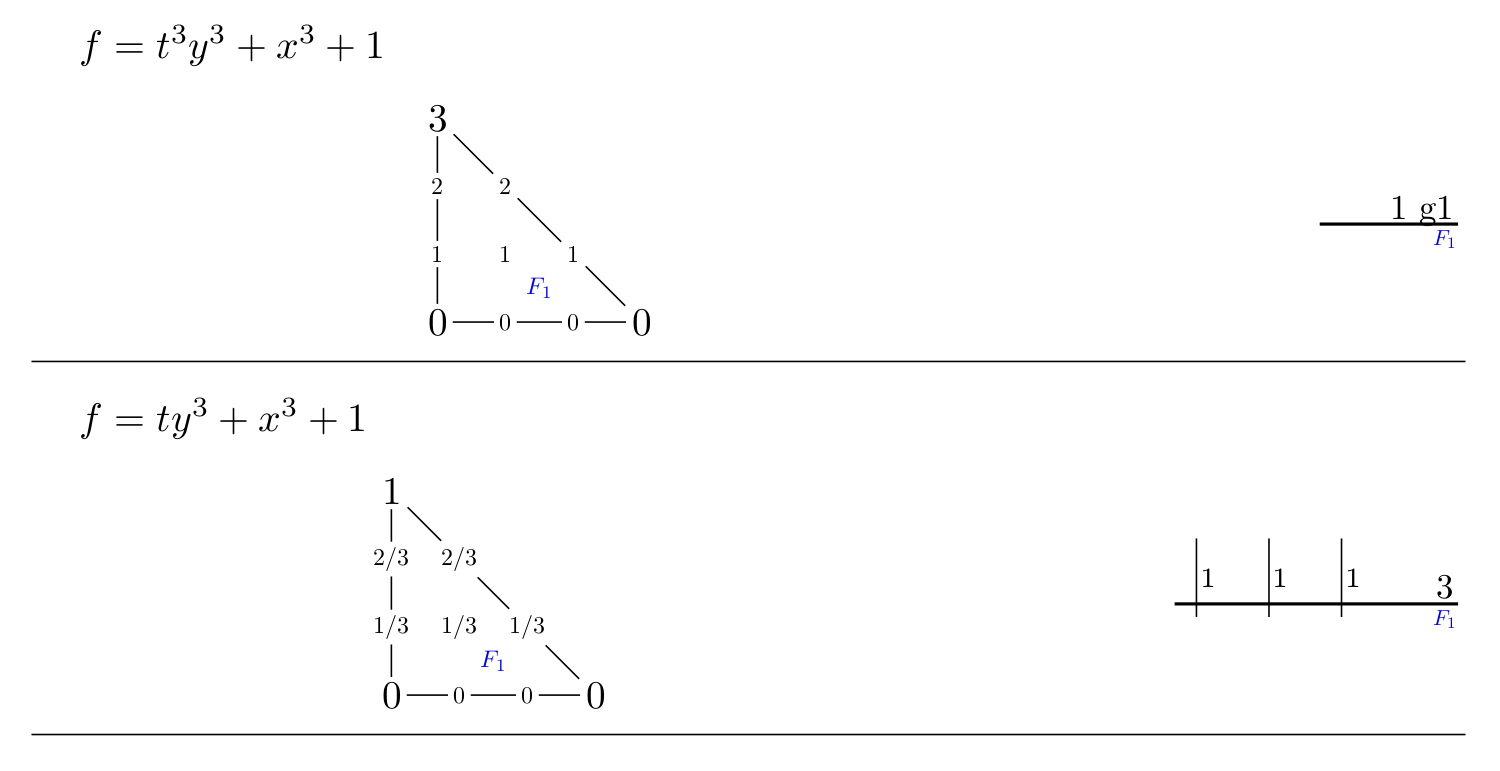
\includegraphics[width=\textwidth]{examples}
\caption[Caption for example]{Partitions of the Newton polygons and the associated graphs of the special fibers corresponding to the equations $f_1 = t^3 y^3 + x^3 + 1$ and $f_2 = t y^3 + x^3 + 1$. (Image created via the software Magma\textsuperscript{1} using scripts by Tim Dokchitser to compute toric models\textsuperscript{2}).
\\
\small\textsuperscript{1} \url{https://magma.maths.usyd.edu.au/magma/}
\\
\small\textsuperscript{2} \url{https://people.maths.bris.ac.uk/~matyd/newton/}}
\end{figure}
\end{example}

\begin{theorem}[Dor18, Thm. 3.13]
Let $f \in K[x^{\pm 1}, y^{\pm 1}]$ be any Laurent polynomial defining a 1-dimensional scheme $C_0 = U_f \subset \Gm{K}^2$. Then $\C_\Delta / R$ is a (proper, flat) model of the toric completion $C = C_0^\Delta$ with respect to the Newton polygon $\Delta = \Delta(f)$. The special fiber $\C_\kappa$ is a union of closed subschemes $\overline{X}_F$ indexed by $\nu$-faces $F$ and chains $X_L \times_\kappa \Gamma_L$ where $\Gamma_L$ is a union of $\P^1_{\kappa}$ intersecting transversally as follows:
\begin{enumerate}
\item for each $\nu$-edge $F$: the scheme $\overline{X}_F$ has multiplicity $\delta_F$ and, via Theorem \ref{baker_refinement}, are geometrically connected and have arithmetic genus $ g_F = |\{ P \in F^\circ \cap \Z^2 \mid \nu(P) \in \Z \} | $.
\item for each $\nu$-edge $L$ choose a sequence $\frac{m_i}{d_i} \in \Q$ ($0 \le i \le r+1$) then let $\Gamma_L = \Gamma^1_L \cup \cdots \cup \Gamma^r_L$ with each $\Gamma^i_L$ isomorphic to $\P^1_k$ embedded with multiplicity $\delta_L d_i$ and meeting transversally where we identify $0 \in \Gamma^i_L$ with $\infty \in \Gamma^{i+1}_L$. If $r = 0$ then let $\Gamma_L = \Spec{k}$.
\item The subscheme $X_L \times \{ 0 \} \subset X_L \times \Gamma^1_L$ is identified with $\overline{X}_{F_1} \setminus X_{F_1}$ for the $\nu$-face $F_1$ bordering $L$ and, when $L$ is inner, likewise $X_L \times \{ \infty \} \subset X_L \times \Gamma^r_L$ is identified with $\overline{X}_{F_2} \setminus X_{F_2}$ for the other $\nu$-face $F_2$ bordering $L$. These intersections are transversal and, in fact, as a scheme the intersection is $V(\overline{f_L}^{\delta_L}) \subset X_L \subset \overline{X}_F$. 
\end{enumerate}
Furthermore, the geometrically regular locus of $\C_\Delta$ contains,
\begin{enumerate}
\item the smooth locus of $X_F$, for each $\nu$-face $L$
\item the smooth locus of $X_L \times \Gamma_L$, for each $\nu$-edge $L$
\item the smooth points of $\overline{X}_F \setminus X_F$ corresponding to $L$ when $L \subset \partial F$ is an outer edge with $\delta_L = \delta_F$ and $r = 0$. 
\end{enumerate}
Finally, if $C_0$ is $\Delta_\nu$-regular then $C = C_0^\Delta$ is smooth and thus the unique smooth proper curve birational to $C_0$ and $\C_\Delta / R$ is a regular normal crossings model of $C$. 
\end{theorem}

\section{Relationships Between Toric Notions of Regularity}

We have discussed a number of regularity conditions on curves originating from their compatibility in some sense with a certain set of toric embeddings. The utility of these conditions is that they can be verified from an equation defining some affine model of the curve in $\Gm{k}^2$. Although these notions are clearly related, we here show that they are, indeed, inequivalent. In this situation, we have a discrete valued field $K$ with valuation ring $R$ and residue field $\kappa$. On the special fiber, we will distinguish between the arithmetic ($\kappa$ non-algebraically closed) and geometric ($\kappa$ arithmetically closed) situations. 

\begin{prop}
Let $C$ be a smooth curve over $K$. Then we have the following implications,
\begin{center}
\begin{tikzcd}
C \text{ is strict } \Delta_\nu \text{-regular} \arrow[Rightarrow, r] \arrow[Rightarrow, d] & C \text{ is nondegenerate } \arrow[Rightarrow, d] 
\\
C \text{ is } \Delta_\nu \text{-regular} \arrow[Rightarrow, r] & C \text{ is weakly nondegenerate}
\end{tikzcd}
\end{center}
Furthermore, no implication is reversible. 
\end{prop}

\begin{proof}
The fact that $\Delta$-nondegeneracy implies weak $\Delta$-nondegeneracy is simply an application of Baker's theorem (recall that this notion was created, by design, as a weaker form of $\Delta$-nondegeneracy, hence the name).  Note that the outer-regular condition introduced in the definition of $\Delta_\nu$-regularity is satisfied when $\overline{X}_F$ is smooth. Thus, $\Delta_\nu$-regularity implies $\Delta_\nu$-regularity since when each of $X_F$ and $X_L$ is smooth then $\overline{X}_F$ is smooth as well via Baker's theorem. 
\par
Strict $\Delta_\nu$-regularity implies that each $X_L$ is smooth thus satisfying the conditions of $\Delta$-nondegeneracy.
Finally, $\Delta_\nu$-regularity implies weak nondegeneracy by the main theorem since if $C_0$ is an affine model in $\Gm{k}^2$ then $C_0^\Delta$ is smooth. Therefore, the affine equation is weakly $\Delta$-nondegenerate with the added condition that $\Delta = \Delta(f)$. Notice that the outer-regularity condition in the definition of a $\Delta_\nu$-regular equation corresponds exactly to the smoothness hypothesis in weak $\Delta$-regularity. So see that strict $\Delta_\nu$-regularity and $\Delta_\nu$-regularity of an equation are not equivalent, let $f \in K[x^{\pm 1}, y^{\pm 1}]$ be a weakly $\Delta$-nondegenerate Laurent polynomial with every term having zero valuation. Then, there is a unique face $F = \Delta(f)$ and for each edge we have $\delta_F = \delta_L = 1$. Then $f$ is $\Delta_\nu$-regular iff it is outer-regular i.e. $U_f^\Delta \subset \Toric_\Delta$ is smooth so $f$ is weakly $\Delta(f)$-nondegenerate. We have seen that weakly $\Delta$-nondegenerate equations need not be $\Delta$-nondegenerate. 
\par
We will give examples showing that nondegenerate curves need not be $\Delta_\nu$-regular.
\end{proof}

\subsection{Genus One Example}

In the arithmetic case, the form of the Galois action on the special fiber comprises an obstruction to having the sort of toric-constructed model described in the previous section. Specifically, the Galois action on the dual graph only permutes ``parallel'' chains of components isomorphic to $\P^1$ therefore each component $\overline{X}_F$ for the faces $F$ must be Galois-invariant, in particular, this includes all positive genus components. Furthermore, note that each component $\overline{X}_F$ is geometrically connected and, by Baker's theorem, smooth when in the $\Delta_\nu$-regular case. Therefore, the special fiber of regular normal-crossings models of $\Delta_\nu$-regular curves cannot have nontrivial orbits of positive genus irreducible components.  
\bigskip\\
To illustrate this phenomenon, we consider the following example. We consider the equicharacteristic case with a section $\kappa \to R$. Choose the ambient scheme,
\[ \P^1_R \times_R \P^1_R = \Proj{R[X_0, X_1]} \times_R \Proj{R[Y_0, Y_1]} \]
and an element $q \in \kappa$. Then we consider the closed subscheme,
\[ X = V((X_0^2 - q X_1^2)(Y_0^2 - q Y_1^2) - \varpi X_0 X_1 Y_0 Y_1) \subset \P^1_R \times_R \P^1_R \] 
where $\varpi \in R$ is the uniformizer. Then $X \to \Spec{R}$ is a regular normal-crossings model of
\[ X_K = V((X_0^2 - q X_1^2)(Y_0^2 - q Y_1^2) - \varpi X_0 X_1 Y_0 Y_1) \subset \P^1_K \times_K \P^1_K \]
This is a smooth curve in $\P^1_K \times_K \P^1_K$ of bidegree $(2, 2)$ and thus genus $g = 1$.
This curve has an affine model,
\[ U = \Spec{k[x, y]/((x^2 - q)(y^2 - q) - \varpi xy)} \subset \A^1_K \times_K \A^1_K \]
Now we consider the special fiber,
\[ X_\kappa = V(X_0^2 - q X_1^2) \cup V(Y_0^2 - q Y_1^2) \subset \P^1_\kappa \times_\kappa \P^1_\kappa \]
The behavior of the special fiber depends on whether $q \in \kappa$ is a square. When $q$ is a non-square, the special fiber has two components $C_1, C_2$ which intersect at two points,
\[ P_{\pm} = (X_0^2 - q X_1^2, Y_0^2 - q Y_1^2, X_0 \mp Y_0) \]
each of order two so $C_i \cdot C_i = -4$ and $[\kappa(C_i) : \kappa] = 2$. Therefore, from the genus formula $g_C = 1$ agreeing with our previous result. Geometrically, each component of the special fiber bifurcates to give four components $C_i$ arranged in a square. Then $C_i \cdot C_i = -2$ since each intersects two other components with a simple intersection so again $g_C = 1$. However, there is a Galois action which flips the square along its diagonal exchanging the opposite pairs of intersection points.
\begin{figure} \label{example_with_P1s}
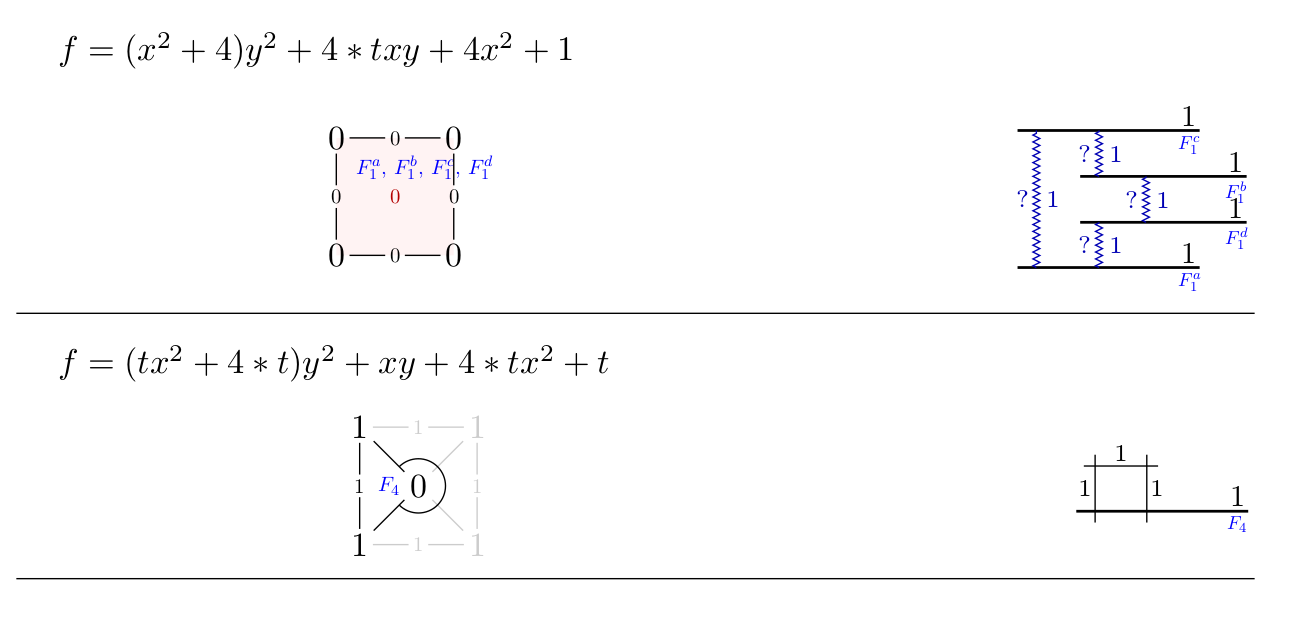
\includegraphics[width=\textwidth]{P1_example}
\caption[Caption for example]{The algorithm applied to $f_1 = (x^2 - 1)(y^2 - 1) - t xy$ and the change of variables $f_2 = uv - t (x^2 - 1)(y^2 - 1)$ chosen to ensure $\Delta_\nu$-regularity. Notice the point of failure of $\Delta_\nu$-regularity in the first case is the singularity of the special fiber which is determined by a single face in this affine presentation. Furthermore, note the topology of the special fiber when it is properly computed. $\Delta_\nu$-regular models are only capable of producing this special fiber in the geometric case i.e. when the components are Galois fixed which occurs when $q \in \kappa$ is a square. However, regardless of $q$, the topology of the special fiber is unchanged with the arithmetic information being encoded in the Galois action instead. (Images created via the software Magma\textsuperscript{1} using scripts by Tim Dokchitser to compute toric models\textsuperscript{2}).
\\
\small\textsuperscript{1} \url{https://magma.maths.usyd.edu.au/magma/}
\\
\small\textsuperscript{2} \url{https://people.maths.bris.ac.uk/~matyd/newton/}}
\end{figure}
\bigskip\\
When $q \in \kappa$ is a non-square, the Galois action on the special fiber does not fix any irreducible component and thus cannot be of the type produced by the previously given toric construction. Therefore, this Galois action may provide an obstruction to finding a $\Delta_\nu$-regular affine equation for $X_K$ despite the fact that we have produced a manifestly $\Delta$-toric affine equation for $X_K$ since $X_K$ is embedded in $\P^1_K \times_K \P^1_K$  via the usual compactification of $f = (x^2 - q)(y^2 - q) - \varpi xy$ with respect to its Newton polygon. To be specific, the r.n.c. model $X$ of the curve $X_K$ cannot be one produced by a $\Delta_\nu$-regular equation. However, the special fiber $X_\kappa$ contains no exceptional curves of the first kind so this is actually a minimal model. In particular, any r.n.c. of $X_K$ may be blown down to $X$. Thus, if $X_K$ had a $\Delta_\nu$-regular equation, this would produce a r.n.c. model $\C_\Delta$ of $X_K$ which can then be blown down to $X$. However, the components of the special fiber of $\C_\Delta$ has fixed points under the $\Gal{\kappa^\sep / \kappa}$-action and thus so does $X_K$. This gives an example of a genus one toric curve (genus one curves are \textit{a priori} toric in any case) which is never-the-less not $\Delta_\nu$-regular.
\bigskip\\
In the case that $q \in \kappa$ is a square, say for definiteness $q = 1$, then the special fiber $X_\kappa$ has the same structure as in the geometric picture except with trivial Galois action. It is easy to show that no matter if $q \in \kappa$ is a square or not, the affine equation $f = (x^2 - q)(y^2 - q) - \varpi xy$ is never $\Delta_\nu$-regular because there is a single face which is non-smooth after reduction to $\kappa$. However, in this case this a pathology of the specific choice of affine equation rather than the curve $X_K$. Indeed, performing a change of variables $u_{\pm} = \tfrac{1}{2}(X_0 \pm X_1)$ and $v_{\pm} = \tfrac{1}{2}(Y_0 \pm Y_1)$ which does correspond automorphism of $\P^1_k \times_k \P^1_k$ but not of the torus $\Gm{k}^2$ reflecting the fact that the necessary change of variables must shift the location of the toric divisor in order to be $\Delta_\nu$-regular. Then the homogeneous equation becomes, 
\[ \tilde{f} = 16 u_+ u_{-} v_{+} v_{-} - \varpi (u_{+}^2 - u_{-}^2) (v_{+}^2 - v_{-}^2) \]
Taking the affine patch $D_{+}(u_{-}) \times D_+(v_{-})$ gives an affine model,
\[ U = \Spec{k[u,v]/(16 uv - \varpi (u^2 - 1)(v^2 - 1)} \]
Furthermore, for $p \neq 2$ this equation is $\Delta_\nu$-regular. 


\subsection{Genus Five Example}


In order to extend our argument to higher genus curves, we need to apply Riemann-Roch. However, since this example only works in the arithmetic setting we require a slight modification to the standard statement of Riemann-Roch found in Hartshorne \cite[Thm. IV.1.3]{har}. To ensure there is no confusion, we will provide a proof here.

\begin{theorem}[Riemann-Roch]
Let $X$ be a smooth proper curve over $k$ with $H^0(X, \struct{X}) = K$ and genus $g = \dim_K H^0(X, \omega_X)$. Then for any line bundle $\L$,
\[ \chi(\L) = \dim_k H^0(X, \L) - \dim_k H^0(X, \omega_X \otimes_{\struct{X}} \L^\vee) = \deg{\L} + [ K : k ] (1 - g) \]
Where $\deg{\L}$ is defined in the arithmetic case as follows. Choose a nonzero meromorphic section $s \in H^0(X, \L \otimes_{\struct{X}} \K_X)$ and a local trivialization $\{ (U_i, s_i) \}$ with $s_i \in \L(U_i)$ such that $\struct{U_i} \xrightarrow{s_i} \L|_{U_i}$ is an isomorphism. Then define,
\[ \deg{\L} = \sum_{P \in X} [\kappa(P) : k] \: \ord_{P}(s/s_i) \] 
for some $i$ with $P \in U_i$. 
\end{theorem}

\begin{proof}
First, note that by Serre duality, $H^1(X, \L) \cong H^0(X, \omega_X \otimes_{\struct{X}} \L^\vee)^\vee$ so,
\[ \chi(\L) = \dim_k H^0(X, \L) - \dim_k H^1(X, \L) = \dim_k H^0(X, \L) - \dim_k H^0(X, \omega_X \otimes_{\struct{X}} \L^\vee) \]
Since $X$ is smooth, every line bundle $\L$ is $\struct{X}(D)$ for some divisor $D$. However, since $X$ is smooth, the map $c_1 : \Pic{X} \to \Cl{X}$ is an isomorphism sending,
\[ \L \mapsto \sum_{P \in X} [P] \: \ord_{P}(s_i / s) \]
where the sections $s_i$ and $s$ are as before. Therefore, for a divisor,
\[ D = \sum_{P \in X} n_P \: [P] \]
if we define the degree (including the arithmetic degrees of extensions),
\[ \deg{D} = \sum_{P \in X} [\kappa(P) : k] \: n_P \]
then clearly $\deg{\L} = \deg{c_1(\L)}$. Since $c_1$ is an isomorphism, it suffices to show that,
\[ \chi(\struct{X}(D)) = \deg{D} + 1 - g \]
However, every divisor $D$ can be obtained by a finite sequence of adding or subtracting points $[P]$ from $D = 0$ i.e. from the line bundle $\struct{X}$. Furthermore,
\[ \chi(\struct{X}) = \dim_k H^0(X, \struct{X}) - \dim_k H^1(X, \struct{X}) = [K : k] (1 - g) \]
since, by Serre duality, $\dim_k H^1(X, \struct{X}) = \dim_k H^0(X, \omega_X) = [K : k] g$ because $\dim_K H^0(X, \omega_X) = g$ by definition. Therefore, to proceed by induction, it suffices to show that,
\[ \chi(\L \otimes_{\struct{X}} \struct{X}(\pm P)) = \chi(\L) \pm [\kappa(P) : k] \]
since $\deg{(\L \otimes \struct{X}(\pm P))} = \deg{\L} \pm [\kappa(P) : k]$. Consider the exact sequence,
\begin{center}
\begin{tikzcd}
0 \arrow[r] & \struct{X}(-P) \arrow[r] & \struct{X} \arrow[r] & (\iota_P)_* \kappa(P) \arrow[r] & 0
\end{tikzcd}
\end{center}
where $\kappa(P)$ is the structure sheaf of $P$ as a reduced closed subscheme. Then tensoring by $\L$ we get,
\begin{center}
\begin{tikzcd}
0 \arrow[r] & \L \otimes_{\struct{X}} \struct{X}(-P) \arrow[r] & \L \arrow[r] & (\iota_P)_* \kappa(P) \arrow[r] & 0
\end{tikzcd}
\end{center}
since $\L$ is locally free so $(\iota_P)_* \kappa(P) \otimes_{\struct{X}} \L = (\iota_P)_* \kappa(P)$. Thus,
\[ \chi(\L) = \chi(\L \otimes_{\struct{X}} \struct{X}(-P)) + \chi((\iota_P)_* \kappa(P)) \]
however
\[ \chi(\kappa(P)) = \dim_k H^0(X, (\iota_P)_* \kappa(P)) - \dim_k H^1(X, (\iota_P)_* \kappa(P)) = \dim_k \kappa(P) = [\kappa(P) : k] \]
Therefore,
\[ \chi(\L \otimes_{\struct{X}} \struct{X}(-P)) = \chi(\L) - [\kappa(P) : k] \]
Likewise, replacing $\L$ by $\L \otimes_{\struct{X}} \struct{X}(P)$ we see that,
\[ \chi(\L \otimes_{\struct{X}} \struct{X}(P)) = \chi(\L) + [\kappa(P) : k] \]
proving the theorem. 
\end{proof}

\begin{rmk}
If $s \in H^0(X, \L)$ is a nonzero global section, then we can compute $\deg{\L}$ using the vanishing of $s$ which is effective since $s$ has no poles. Thus, $\deg{\L} \ge 0$. In particular, applying Riemann-Roch to $\omega_X$ we see that $\deg{\omega_X} = \chi(\omega_X) - \chi(\struct{X}) = g - 1 - (1 - g) = 2 g - 2$. Therefore, if $\deg{\L} > 2 g - 2$ then $\deg{(\omega_X \otimes_{\struct{X}} \L^\vee)} = 2 g - 2 - \deg{\L} \le 0$ which implies that $H^0(X, \omega_X \otimes_{\struct{X}} \L^\vee) = 0$ so by Riemann-Roch applied to $\L$ we find,
\[ \dim_k H^0(X, \L) = \deg{\L} + 1 - g \]
\end{rmk}
\noindent\\
Now we consider the following example. Take the field $K = \Fin_p(t)$ with valuation ring $R = \Fin_p[t]_{(t)}$ and residue field $\kappa = \Fin_p$. Given an elliptic curve $C_K$ over $K$ with good reduction $C$ over $\kappa$ so we may take a smooth model $\C$ over $R$. For example, let $q \in \Fin_p^\times$ be a generator, take 
\[ C_K = \Proj{K[X, Y, Z]/(Y^2 Z - X(X^2 - q Z^2)} \] 
we may take the model,
\[ \C = \Proj{R[X, Y, Z]/(Y^2 Z - X(X^2 - q Z^2)} \] 
which is smooth and proper over $R$ for $p \neq 2$. Clearly $\C_K = C_K$ and the special fiber $\C_\kappa$ is the smooth reduction. Now let $P$ be a $\Fin_{p^2}$-point of $C$ which is not a $\Fin_p$-rational points, e.g. take $P = (X^2 - q Z^2, Y)$ which has $\kappa(P) = \Fin_{p^2}$. Recall that $\omega_C = \struct{C}$ since $C$ is an abelian variety and $g = 1$ so if $\deg{\L} > 0$ we know that $\dim_k H^0(C, \L) = \deg{\L}$ be Riemann-Roch. Then consider the line bundle $\L = \struct{C}(P)$ then $\deg{\L} = [\kappa(P) : k]  = 2$. Therefore, we can choose linearly independent sections $s_0, s_1 \in H^0(C, \L)$ where the section $s_0 : \struct{C} \to \L$ is the canonical section defining the closed subscheme $P$ from the inclusion $\L^\vee \to \struct{C}$ of the sheaf of ideals of $P$. Then $s_0$ vanishes exactly on $P$ i.e. the closed subscheme $V(s_0) = P$. Now $\div{(s_1)}$ is an effective divisor of degree $2$ so either $\div{(s_1)} = [P]$ or $\div{(s_1)} = [Q_1] + [Q_2]$ for $\Fin_p$-rational points $Q_1, Q_2$ or $\div{(s_1)} = [Q]$ where $Q \neq P$ is an order-$2$ point. However, if $\div{(s_1)} = [P]$ then $s_1$ must have vanishing order $1$ since it has degree $2$ which implies that $s_0 / s_1 \in H^0(C, \struct{C}^\times)$ contradicting the fact that $s_0$ and $s_1$ are independent in $H^0(C, \L)$ (over $H^0(C, \struct{C}) = \kappa$). The takeaway is that $s_0$ only vanishes at $P$ and $s_1$ does not vanish at $P$. Notice, since we are in equicharacteristic the map $\kappa \to R$, our model is simply a base-change,
\[ \C = C \times_{\Spec{\kappa}} \Spec{R} \]
so we get a line bundle $\L' = \pi_1^* \L$ on $\C$ and, by Kunneth, $H^0(\C, \L') = H^0(C, \L) \otimes_\kappa R$.   
\bigskip\\
We now construct our example as follows. Consider the scheme $\C \times_R \C$ and denote the projection maps, $\pi_i : \C \times_R \C \to \C$. Take the section,
\[ \pi_1^* s_0 \otimes \pi_2^* s_0 - t \: \pi_1^* s_1 \otimes \pi_2^* s_1 \in H^0(\C \times_R \C, \pi_1^* \L' \otimes_{\struct{X}} \pi_2^* \L') \]
on the bundle $\L' \boxtimes \L' := \pi_1^* \L' \otimes_{\struct{X}} \pi_2^* \L'$. We will write this section as $q = s_0 \boxtimes s_0 - t \: s_1 \boxtimes s_1$. Then we take,
\[ X = V(s_0 \boxtimes s_0 - t \: s_1 \boxtimes s_1) \subset \C \times_R \C \]
I claim that $X \to \Spec{R}$ is a regular proper model of,
\[ X_K = V(s_0 \boxtimes s_0 - t \: s_1 \boxtimes s_1) \subset C_K \times_K C_K \]
Here $C_K$ is an elliptic curve over $K$ and I claim that $X_K$ is a smooth projective curve over $K$ of genus $g = 9$. To show this, we compute an affine curve birational to $X_K$. First, we compute the sections $s_0, s_1 \in H^0(X, \struct{C}(P)) \subset K(C)$. Recall that,
\[ H^0(X, \struct{X}(P)) = \{ f \in K(X) \mid \div{(f)} + P \ge 0 \text{ or } f = 0 \} \]
and the canonical section is $s_0 = 1$. Then take $s_1 = \frac{Z}{Y}$ which has, 
\[ \div{(s_1)} = 2 [\infty] - [P] \]
where $[\infty] = [0 : 1 : 0]$ is the point at infinity in the standard $(x, y) = (\frac{X}{Z}, \frac{Y}{Z})$ coordinates\footnote{For $P = (X^2 - g Z^2, Y)$ the intuitive choice $s_1 = (\frac{X^2}{Z^2} - q)^{-1}$ will not give a section of $\struct{C}(P)$ because its vanishing order is too large, in fact, $\ord_{P}{(\frac{X^2}{Z^2} - q)} = 2$. To see this, consider the affine patch $D_{+}(Z)$ with coordinates $(x, y) = (\frac{X}{Z}, \frac{Y}{Z})$ and the section $(x^2 - q) \in A_{P}$ where $A = \kappa[x, y]/(y^2 - x(x^2 - q))$. Let $\m = P A_P$ then clearly $(x^2 - q) \in \m$ but also $(x^2 - q) \in \m^2$ because $x^{-1} y^2 = (x^2 - q) \in \m^2$ since $y \in \m$ and $x \notin P$.}. To compute $\div{(s_1)}$, note that $\ord_{P}(y) = 1$ because $y \in (x^2 - q, y)$ but $y \notin (x^2 - q, y)^2$, furthermore, in $D_+(Y)$ and local coordinates $(x,z) = (\frac{X}{Y}, \frac{Z}{Y})$ then $s_1 = z$ and $\ord_{\infty}(z) = 2$ because $z \in (x, z)$ and $z \in (x, z)^2$ since $z = x(x^2 - q z^2) \in (x, z)^2$. 
\bigskip\\
We choose the affine patch, $U_K \times_K U_K \subset C_K \times_K C_K$ which is defined by,
\[ U_K = C_K \cap D(Z) = \Spec{K[x,y]/(y^2 - x(x^2 - q))} \]
Since $\div{(\frac{Y}{Z})} = [P] - 2 [\infty]$, applying the exact sequence,
\begin{center}
\begin{tikzcd}
\lbrack \infty \rbrack \cdot \Z \arrow[r] & \Cl{C_K} \arrow[r] &  \Cl{U_K} \arrow[r] & 0
\end{tikzcd}
\end{center}
we see that $[P] \in \Cl{U}$ is principal $[P] = \div{(\frac{Z}{Y})}|_U$. Therefore, $\struct{C_K}(P) \cong \struct{C_K}$ via the isomorphism, $1 \mapsto \frac{Y}{Z}$ meaning that $s_0 \mapsto \frac{Y}{Z}$ and $s_1 \mapsto 1$ in $\struct{C_K}$. Therefore, the affine open,
\[ V_K = V(s_0 \boxtimes s_0 - t \: s_1 \boxtimes s_1) \subset U_K \times_K U_K \]
is explicitly,
\[ V_K = \Spec{K[x_1, y_1, x_2, y_2]/(y_1^2 - x_1(x_1^2 - q), y_2^2 - x_2(x_2^2 - q), y_1 y_2 - t)} \]
In the software sage\footnote{\url{http://www.sagemath.org/}}, we can compute the genus $g = 5$ from this affine presentation \footnote{In fact, asking sage to compute the genus of the above affine curve produces $g = 10$. This reflects that sage computes the genus \textit{over the field of definition} where as we take the base field here to be $k = H^0(X, \struct{X})$ and define $g = \dim_k H^0(X, \Omega^1_X)$. In our example here, since $P$ is an order two point, $H^0(X, \struct{X}) = \Fin_{p^2}$ and thus, the correct genus is computed as,
\[ g(X) = \dim_\kappa H^0(X, \Omega^1_X) / \dim_\kappa H^0(X, \struct{X}) = 10/2 = 5 \]}.
Now consider the special fiber $X_\kappa = V(s_0 \boxtimes s_0) \subset C \times_k C$ given by the base change under the map $R \to R/(t) = \kappa$ sending $t \mapsto 0$. Therefore, the irreducible components $C_1, C_2$ are each isomorphic to $C \times_{\Fin_p} \Fin_{p^2}$ and as effective Cartier divisors $X_\kappa = C_1 + C_2$ with multiplicity one since the special fiber is reduced. The intersection number between these components is $C_1 \cdot C_2 = 4$ because these components intersect at two points $P_{\pm} = (X_0^2 - q Z_0^2, Y_0, X_1^2 - q Z_1^2, Y_1, X_0 \mp X_1)$ each a point of degree $2$. Therefore, using $C_i \cdot (C_1 + C_2) = 0$ we find that $C_i \cdot C_i = -4$. Therefore, applying the genus formula,
\[ g_C = 1 + \sum_{i = 1}^n m_i \left( [\kappa(C_i) : \kappa] (g_{C_i} - 1) - \frac{1}{2} (C_i \cdot C_i) \right) \]
we get $g_C = 1 + 4 = 5$ since $g_{C_i} = 1$ and $m_i = 1$ because each component is a reduced elliptic curve. 
\bigskip\\
Geometrically, each component bifurcates to give a square with each side a reduced elliptic curve divisor isomorphic to $C$. The Galois group acts on this square by reflection across the diagonals. Since $X$ does not contain any exceptional curves of the first kind, it is the minimal model of $V$ (and in fact the minimal regular normal crossings model since $X_\kappa$ happens to be a normal crossings divisor). Therefore, any proper regular normal crossings model of $V$ must be a blowup of $X$ and, in particular, its special fiber must contain two pairs of Galois conjugate elliptic curves. Therefore, no $\Delta_\nu$-regular affine equation for $V$ can exist since such an equation would define a proper regular normal crossings model of $V$ with trivial Galois action on positive genus components. 



\section{Appendix}

\subsection{Curves and Genera}

\begin{lemma}
Let $X$ be a integral scheme proper over $k$ then $K = H^0(X, \struct{X})$ is a finite field extension of $k$ and for any coherent $\struct{X}$-module $\F$, the cohomology $H^p(X, \F)$ is a finite-dimensional $H^0(X, \struct{X})$-module.
\end{lemma}

\begin{proof}
Since $\struct{X}$ is coherent, and $X$ is proper over $k$ so $K = H^0(X, \struct{X})$ is a finite $k$-module. However, since $X$ is integral $H^0(X, \struct{X})$ is a domain but a finite $k$-algebra domain is a field and we see $K / k$ is a finite extension of fields. Furthermore, the $\struct{X}(X)$-module structure on $H^p(X, \F)$ gives it a $K$-module structure. Since $X$ is proper over $k$ then $H^p(X, \F)$ is a finite $k$-module and thus finite as a $K$-module.
\end{proof}

\begin{rmk}
When $k$ is not algebraically closed then we may not have $H^0(X, \struct{X}) = k$ even for smooth projective varieties. Therefore, some caution must be taken in defining numerical invariants of the curve such as genus. However, by \cite[\href{https://stacks.math.columbia.edu/tag/0BUG}{Tag 0BUG}]{stacks-project}, whenever $X$ is proper geometrically integral then indeed $H^0(X, \struct{X}) = k$. Furthermore, for proper $X$ if $H^0(X, \struct{X}) \neq k$ then $X$ cannot be geometrically connected by \cite[\href{https://stacks.math.columbia.edu/tag/0FD1}{Tag 0FD1}]{stacks-project}.
\end{rmk}

\begin{defn}
Let $C$ be a smooth proper curve over $k$ with $H^0(C, \struct{C}) = K$. Then we define the \textit{genus} $g(C) := \dim_K H^0(X, \Omega_{C / k})$. If $C$ is a geometrically irreducible curve over $k$ then there is a unique normal proper curve $S$ over $k$ birational to $C$. If $S$ is smooth, we define $g(C) := g(S)$. If $k$ is not perfect, then $S$ may not be smooth. However, under a finite purely separable extension $K / k$, since $C_K$ is a irreducible, we can ensure that $(C_K)_{\red}$ admits a smooth proper model $S'$ over $K$. Then we define $g(C) := g(S')$.
\end{defn}

\begin{rmk}
By definition, the genus of a curve is clearly a birational invariant since there is a unique smooth complete curve in every birational equivalence class of curves. 
\end{rmk}

\begin{defn}
The \textit{arithmetic genus} $g_a(C)$ of a proper curve $C$ over $k$ with $H^0(C, \struct{C}) = K$ is,
\[ g_a(C) := \dim_K H^1(X, \struct{C}) \]
By Serre duality, if $C$ is smooth then $H^0(C, \Omega_C) = H^1(C, \struct{X})^\vee$ meaning that $g_a(C) = g(C)$. 
\end{defn}

\begin{rmk}
The arithmetic genus depends on the projective compactification and singularities meaning it will not be a birational invariant unlike the (geometric) genus. 
\end{rmk}

\begin{example}
Let $k = \Fin_p(t)$ for an odd prime $p = 2k + 1$ and consider the curve,
\[ C = \Spec{k[x,y]/(y^2 - x^p - t)} \]
which is regular but not smooth at $P = (y, x^p - t)$. Consider the purely inseperable extension $K = \Fin_p(t^{1/p})$. Then $C_K = \Spec{K[x,y]/(y^2 - (x - t^{1/p})^p)} \cong \Spec{K[x,y]/(y^2 - x^p)}$. Taking the normalization of $C_K$ gives $\A^1_K \to C_K$ via $t \mapsto (t^p, t^2)$. This is birational since the following ring map is an isomorphism,
\[ (K[x,y]/(y^2 - x^p))_{x} \to K[t]_{t} \]
sending $x \mapsto t^2$ and $y \mapsto t^p$ which has an inverse $t \mapsto y/x^k$ since $x \mapsto t^2 \mapsto y^2/x^{2k} = x$ and $y \mapsto t^p \mapsto y^{p}/x^{kp} = y (y^{2k}/x^{pk}) = y$ and $t \mapsto y/x^k \mapsto t^{p - 2k} = t$. 
\bigskip\\
Therefore, $C_K \birat \P^1_K$ so $g(C) = g(C_K) = 0$. However, consider the projective closure,
\[ \overline{C} = \Proj{k[X,Y,Z]/(Y^2 Z^{p-2} - X^p - t Z^p)} \]
then $\overline{C} \embed \P^2_k$ is a Cartier divisor (since $\P^2_k$ is locally factorial) so we find that $H^0(\overline{C}, \struct{\overline{C}}) = k$ and $\dim_k H^1(\overline{C}, \struct{\overline{C}}) = \tfrac{1}{2}(p-1)(p-2) = k (2k - 1)$ since its sheaf of ideals is $\struct{\P^2_k}(-p)$. Then $p = 3$ we expect this to be an elliptic curve and we do see $g_a(\overline{C}) = 1$. However, $g(\overline{C}) = 0$ and correspondingly $C$ is not smooth due to the positive characteristic phenomenon. 
\end{example}

\begin{lemma}
Suppose that $f : X \to Y$ is a finite birational morphism of $n$-dimensional irreducible Noetherian schemes. Then $H^n(Y, \struct{Y}) \onto H^n(X, \struct{X})$ is surjective.
\end{lemma}

\begin{proof}
The map $f$ must restrict on some open subset $U \subset X$ to an isomorphism $f|_U : U \to V$. Thus, the sheaf map $f^\# : \struct{Y} \to f_* \struct{X}$ restricts on $V$ to an isomorphism $\struct{Y}|_V \xrightarrow{\sim} (f_* \struct{X})|_V$. We factor this map into two exact sequences,
\begin{center}
\begin{tikzcd}
0 \arrow[r] & \K \arrow[r] & \struct{Y} \arrow[r] & \I \arrow[r] & 0
\\
0 \arrow[r] & \I \arrow[r] & f_* \struct{X} \arrow[r] & \Csh \arrow[r] & 0
\end{tikzcd}
\end{center}
with $\K = \ker{(\struct{Y} \to f_* \struct{X})}$ and $\Csh = \coker{(\struct{Y} \to f_* \struct{X})}$ and $\I = \Im{\struct{Y} \to f_* \struct{X}}$. Taking cohomology and using that it vanishes in degree above $n$ we get,
\begin{center}
\begin{tikzcd}
H^{n-1}(Y, \I) \arrow[r] & H^n(Y, \K) \arrow[r] & H^n(Y, \struct{Y}) \arrow[r, two heads] & H^n(Y, \I) \arrow[r] & 0
\\
H^{n-1}(Y, \Csh) \arrow[r] & H^n(Y, \I) \arrow[r] & H^n(X, \struct{X}) \arrow[r, two heads] &  H^n(X, \Csh) \arrow[r] & 0
\end{tikzcd}
\end{center}
where we have used that $f : X \to Y$ is affine to conclude that $H^p(Y, f_* \F) = H^p(Y, \F)$ for any quasi-coherent $\struct{X}$-module $\F$. Furthermore, $\Csh|_V = 0$ so $\Supp{\struct{Y}}{\Csh} \subset X \setminus V$ but $\Csh$ is coherent so the support is closed. Since $V$ is dense open, $\Csh$ is supported in positive codimension so $H^n(Y, \Csh) = 0$ (since $H^n(S, \Csh)$ vanishes due to dimension on the closed subscheme $S = \Supp{\struct{X}}{\Csh}$ on which $\Csh$ is supported). Thus we have,
\[ H^n(Y, \struct{Y}) \onto H^n(Y, \I) \onto H^n(Y, \I) \onto H^n(X, \struct{X}) \]
proving the proposition.
\end{proof}

\begin{lemma} \label{genus_formulas}
Let $S$ and $C$ be proper curves over $k$ where $S$ is smooth which are birationally equivalent and $H^0(S, \struct{S}) \cong H^0(C, \struct{C})$. Then the genera satisfy,
\begin{enumerate}
\item $g_a(C) \ge g_a(S)$
\item $g(C) = g(S)$
\item $g(C) \le g_a(C)$
\end{enumerate} 
where equality holds exactly when $C$ is smooth in which case $C \cong S$.
\end{lemma}

\begin{proof}
Given a birational map $S \birat C$ we can extend it to a birational morphism $S \to C$ since $S$ is regular. The morphism $S \to C$ is automatically finite since it is a non-constant map of proper curves. Then the previous lemma implies that $g_a(S) \le g_a(C)$. (b). follows from the definition of $g(C)$. The third follows from the fact that $g(S) = g_a(S)$  because of Serre duality, 
\[ H^1(S, \struct{S}) \cong H^0(S, \Omega_{S / k})^\vee \]
using that $S$ is smooth. Then we see that $g(C) = g(S) = g_a(S) \le g_a(C)$ proving the inequality part of (c). Finally, if $C$ is smooth we see by Serre duality that $g(C) = g_a(C)$. Conversely, suppose that $g(C) = g_a(C)$ then $g_a(C) = g(C) = g(S) = g_a(S)$ and consider the map $f : S \to C$ which is finite birational map of integral schemes over $k$. In particular, $f$ is affine so for each $y \in C$ we may choose an affine open $y \in V \subset C$ whose preimage $U = f^{-1}(V)$ is also affine. On sheaves, this gives a map of domains $\struct{C}(V) \to \struct{S}(U)$ which localizes to an isomorphism on the fraction fields. However, the localization map of a domain is injective so $\struct{C}(V) \embed \struct{S}(U)$ is an injection. This shows that $\struct{C} \to f_* \struct{S}$ is an injection of sheaves which we extend to an exact sequence,
\begin{center}
\begin{tikzcd}
0 \arrow[r] & \struct{C} \arrow[r] & f_* \struct{S} \arrow[r] & \Csh \arrow[r] & 0
\end{tikzcd}
\end{center} 
Note that $f : S \to C$ induces an isomorphism $H^0(C, \struct{C}) \xrightarrow{\sim} H^0(S, \struct{S})$ since it is a map of fields with the same (finite) dimension over $k$. Then the long exact sequence of cohomology gives,
\begin{center}
\begin{tikzcd}[column sep = small]
0 \arrow[r] & H^0(C, \struct{C}) \arrow[r, "\sim"] & H^0(S, \struct{S}) \arrow[r] & H^0(X, \Csh) \arrow[r] & H^1(C, \struct{C}) \arrow[r, "\sim"] & H^1(S, \struct{S}) \arrow[r] & H^1(S, \Csh) \arrow[r, equals] & 0 
\end{tikzcd}
\end{center}
I claim that $H^1(S, \Csh) = 0$. Since $f$ is birational, $\Csh$ is supported in codimension one. Thus, the map $H^1(C, \struct{C}) \onto H^1(S, \struct{S})$ is surjective but $g_a(C) = g_a(S)$ so these vectorspaces have the same dimension so $H^1(C, \struct{C}) \xrightarrow{\sim} H^1(S, \struct{S})$ is an isomorphism. Thus, from the exact sequence we have $H^0(X, \Csh) = 0$. However, $\Supp{\struct{C}}{\Csh}$ is a closed ($\Csh$ is coherent) dimension zero subset i.e. finitely many discrete closed points. However, a sheaf supported on a discrete set of points is zero iff it has no global sections. Therefore, $\Csh = 0$ so $\struct{C} \xrightarrow{\sim} f_* \struct{S}$. In particular $\struct{C}(V) \xrightarrow{\sim} \struct{S}(U)$ is an isomorphism which implies that the map of affine schemes $f|_U : U \to V$ is an isomorphism. Since the affine opens $V$ cover $C$ we see that $f : S \to C$ is an isomorphism. In particular, $C$ is smooth. 
\end{proof}


\subsection{Extending Rational Maps}

\newcommand{\Nil}{\mathcal{N}}

\begin{lemma}
Regular local rings of dimension $1$ exactly correspond to DVRs.
\end{lemma}

\begin{proof}
Any DVR $R$ has a uniformizer $\varpi \in R$ then $\dim{R} = 1$ and $\m / \m^2 = (\varpi)/(\varpi^2) = \varpi \kappa$ which also has $\dim_{\kappa}(\m / \m^2) = 1$ so $R$ is regular.
Conversely, if $R$ is a regular local ring of dimension $\dim{R} = 1$ then, by regularity, $R$ is a normal Noetherian domain so by $\dim{R} = 1$ then $R$ is Dedekind but also local and thus is a DVR. 
\end{proof}

\begin{proposition}
Let $X$ be a Noetherian $S$-scheme and $Z \subset X$ a closed irreducible codimension $1$ generically nonsingular subset (with generic point $\eta \in Z$ such that $\stalk{X}{\eta}$ is regular). Let $f : X \rat Y$ be a rational map with $Y$ proper over $S$. Then $Z \cap \Dom{f}$ is a dense open of $Z$.
\end{proposition}


\begin{proof}
Choose some representative $(U, f_U)$ for $f : X \rat Y$. Note that $\stalk{X}{\eta}$ is a regular dimension one ring and thus a DVR. Consider the generic point $\xi \in X$ of $X$ then, by localizing, we get an inclusion of the generic point $\Spec{\stalk{X}{\xi}} \to \Spec{\stalk{X}{\eta}} \to X$ and $\stalk{X}{\xi} = K(X) = \Frac{\stalk{X}{\eta}}$. Furthermore, the inclusion of the generic point gives $\Spec{K(X)} \to U \xrightarrow{f_U} Y$ and thus we get a diagram,
\begin{center}
\begin{tikzcd}
\Spec{K(X)} \arrow[d, hook] \arrow[r] & Y \arrow[d]
\\
\Spec{\stalk{X}{\eta}} \arrow[ru, dashed, "\ell"] \arrow[r] & \Spec{k} 
\end{tikzcd}
\end{center}
and a lift $\Spec{\stalk{X}{\eta}} \to Y$ by the valuative criterion for properness applied to $Y \to \Spec{k}$ since $\stalk{X}{\eta}$ is a DVR. Choose an affine open $\Spec{R} \subset Y$ containing the image of $\Spec{\stalk{X}{\eta}} \to Y$ (i.e. choose a neighborhood of the image of $\eta$ which automatically contains $f(\xi)$ since the map factors $\Spec{\stalk{X}{\eta}} \to \Spec{\stalk{Y}{f(\eta)}} \to \Spec{R} \to Y$) and let $\eta \in V = \Spec{A} \subset X$ be an affine open neighborhood of $\xi$ mapping onto $\Spec{R}$. By Lemma \ref{open_domain}, since $\stalk{X}{\eta}$ is a domain, we may shrink $V$ so that $A$ is a domain. Since $X$ is irreducible $U \cap V$ is a dense open. Note that if $\eta \in U$ then $\eta \in \Dom{f}$ and thus $Z \cap \Dom{f}$ is a nonempty open of the irreducible space $Z$ and therefore a dense open so we are done. Otherwise, let $\p \in \Spec{A}$ correspond to $\eta \in Z$ then $A_\p = \stalk{X}{\eta}$ is a  DVR. Take some principal affine open $D(f) \subset U \cap V$ for $f \in A$ so $f \in \p$ since $\p \notin D(f) \subset U \cap V$. Since $A_\p$ is a DVR we may choose a uniformizer $\varpi \in \p$ so the map $A \to \p$ via $1 \mapsto \varpi$ is as isomorphism when localized at $\p$. Since $A$ is Noetherian both are f.g. $A$-modules so there must be some $s \in A \setminus \p$ such that $A_s \to \p_s$ is an isomorphism. Replacing $A$ by $A_s$ we may assume $\p = (\varpi) \subset A$ is principal. Since $f \in \p$ we can write $f = t \varpi^k$ for some $a \in A \setminus \p$ (see Lemma \ref{principal_ideal_powers}). Then consider $\tilde{V} = \Spec{A_t}$. Since $t \notin \p$ then $\eta \in \tilde{V}$ and since $f = t \varpi^k$ we have $D(f) \subset D(t) = \tilde{V}$.
Now we get the following diagram, 
\begin{center}
\begin{tikzcd}[row sep = large]
& & \Spec{R}
\\
\Spec{A_\p} \arrow[rru, bend left, "\ell"] \arrow[r] &  \Spec{A_t} \arrow[ru, dashed, "f_V"]
\\
\Spec{\Frac{A}} \arrow[r] \arrow[u] & \Spec{A_f} \arrow[u] \arrow[ruu, bend right, "f_U"'] 
\end{tikzcd}
\end{center}
I claim the square is a pushout in the category of affine schemes because maps $R \to A_\p$ and $R \to A_f$ which agree under the inclusion to $\Frac{A}$ gives a map $R \to A_\p \cap A_f \subset \Frac{A}$. However, consider,
\[ x \in A_\p \cap A_t \implies x = \frac{u \varpi^r}{s} = \frac{a}{f^n} \]
for $u, s, t \in A \setminus \p$ and $a \in A$. Thus we get,
\[ u t^n \varpi^{r + nk} = s a \]
so $a \in \p^{r + nk} \setminus \p^{r + nk + 1}$ ($s \notin \p$ which is prime) and thus $a = u' \varpi^{r + nk}$ for $u' \in A \setminus \p$. Therefore,
\[ x = \frac{u' \varpi^{r + nk}}{t^n \varpi^{nk}} = \frac{u' \varpi^{r}}{t^n} \in A_t \]
Thus, $A_\p \cap A_f \subset A_f$ so we get a map $R \to A_t$. Therefore we get a map $f_{\tilde{V}} : \tilde{V} \to Y$ such that $(f|_{\tilde{V}})|_{D(f)} = (f_U)|_{D(f)}$ which implies that $\eta \in \tilde{V} \subset \Dom{f}$ so $Z \cap \Dom{f}$ is a dense open of $Z$. 
\end{proof}

\begin{prop}
Let $C \to S$ be a proper regular Noetherian scheme with $\dim{C} = 1$ and $f : C \rat Y$ a rational $S$-map with $Y \to S$ proper. Then $f$ extends uniquely to a morphism $f : C \to Y$. 
\end{prop}

\begin{proof}
For any point $x \notin \Dom{f}$ let $Z = \overline{\{ x \}} \subset D$ for $D = C \setminus \Dom{f}$. Since $\Dom{f}$ is a dense open, we have $\codim{Z, C} \ge \codim{D, C} \ge 1$ but $\dim{C} = 1$ so $\codim{Z, C} = 1$. Furthermore, since $C$ is regular $\stalk{C}{x}$ is regular and thus, by the previous proposition, $Z \cap \Dom{f}$ is a dense open and in particular $x \in \Dom{f}$ meaning that $\Dom{f} = C$ so we get a morphism $C \to Y$. This is unique because $C$ is reduced (it is regular) and $Y$ is separated (it is proper over $S$) so morphisms $C \to Y$ are uniquely determined on any dense open.
\end{proof}

\begin{cor}
Rational maps between normal proper curves are morphisms.
\end{cor}

\begin{cor}
Birational maps between normal proper curves are isomorphisms.
\end{cor}

\begin{proof}
Let $f : C_1 \rat C_2$ and $g : C_2 \rat C_1$ be birational inverses of smooth proper curves. Then we know that these extend to morphisms $f : C_1 \to C_2$ and $g : C_2 \to C_1$. Furthermore, the maps $g \circ f : C_1 \to C_1$ must extend the identity on some dense open. However, since curves are separated and reduced there is a unique extension of this map so $g \circ f = \id_{C_1}$ and likewise $f \circ g = \id_{C_2}$. 
\end{proof}

\begin{thm}
There exists a unique normal curve $C$ over $k$ in each birational equivalence class of curves. If $k$ is perfect then $C$ is smooth.
\end{thm}

\begin{proof}
It suffices to show existence. Given a curve $X$, we consider the projective closure $X \embed \overline{X}$ which is birational and $\overline{X} \to \Spec{k}$ is proper. Then take the normalization $\overline{X}^\nu \to \overline{X}$ which remains proper over $\Spec{k}$ and is birational. Then $\overline{X}^\nu$ is regular and thus smooth over $k$ since $k$ is perfect and $\overline{X}^\nu \to X$ is birational.
\end{proof}

\subsection{General Lemmata}

\begin{lemma} \label{principal_ideal_powers}
Let $A$ be a Noetherian domain and $\p = (\varpi)$ a principal prime. Then any $f \in \p$ can be written as $f = t \varpi^k$ for $f \in A \setminus \p$. 
\end{lemma}

\begin{proof}
From Krull intersection,
\[ \bigcap_{n \ge 0}^\infty \p^n = (0) \]
so there is some $n$ such that $f \in \p^n \setminus \p^{n+1}$. Thus $f = t \varpi^n$ for some $f \in A$ but if $t \in \p$ then $f \in \p^{n+1}$ so the result follows.
\end{proof}


\begin{lemma}
Let $X$ be a Noetherian scheme then $X$ has finitely many irreducible components.
\end{lemma}

\begin{proof}
First let $X = \Spec{A}$ for a Noetherian ring $A$. Then the irreducible components of $A$ correspond to minimal primes $\p \in \Spec{A}$. Then $\dim{A_\p} = 0$ and $A_\p$ is Noetherian so $A_\p$ is Artinian. $A_\p$ must have some associated prime so $\Ass{A_\p}{A_\p} = \{ \p A_\p \}$.  By \cite[\href{https://stacks.math.columbia.edu/tag/05BZ}{Tag 05BZ}]{stacks-project}, then $\Ass{A}{A} \cap \Spec{\A_\p} = \Ass{\A_\p}{\A_\p} = \{ \p \}$ so every minimal prime is an associated prime. However, for $A$ Noetherian then $A$ admits a finite composition series so there are finitely many associated primes.
\bigskip\\
Now let $X$ be a Noetherian scheme. For any affine open $U \subset X$ we have shown that $U$ has finitely many irreducible components. However, since $X$ is quasi-compact there is a finite cover of affine opens and thus $X$ must have finitely many irreducible components. 
\end{proof}

\begin{lemma}
Let $X$ be a Noetherian scheme and $Y$ is the complement of some dense open $U$. Then $\codim{Y, X} \ge 1$.
\end{lemma}

\begin{proof}
It suffices to show that $Y$ does not contain any irreducible component since then any irreducible contained in $Y$ cannot be maximal. Since $X$ is Noetherian, it has finitely many irreducible components $Z_i$. Then if $Z_j \subset Y$ for some $i$ we would have $Z_i \cap U = \varnothing$ but then,
\[ U = \bigcup_{i \neq j} Z_i \]
which is closed so $\overline{U} \subsetneq X$ contradicting our assumption that $U$ is dense.
\end{proof}

\begin{lemma} \label{open_domain}
Let $X$ be a Noetherian scheme and $x \in X$ such that $\stalk{X}{x}$ is a domain. Then there is an affine open neighborhood $x \in U \subset X$ with $U = \Spec{A}$ and $A$ is a domain.
\end{lemma}

\begin{proof}
Take any affine open neighborhood $x \in U \subset X$ with $U = \Spec{A}$ and $\p \in \Spec{A}$ corresponding to $x$. Then $A_\p = \stalk{X}{x}$ is a domain. Since $X$ is Noetherian then $A$ is Noetherian so it has finitely many minimal primes $\p_i$ (corresponding to the generic points of irreducible components of $U$) with $\p_0 \subset \p$. Since $A_\p$ is a domain, it has a unique minimal prime and thus $\p_0$ is the only minimal prime contained in $\p$ (geometrically $A_\p$ being a domain corresponds to the fact that $\p$ is the generic point of a generically reduced irreducible subset which lies in only one irreducible component)
\bigskip\\
Now for any $i \neq 0$ take $f_i \in \p \setminus \p_0$. This is always possible else $\p \subset \p_0$ contradicting the minimality of $\p_0$. If $f \notin \q$ then $\q \not\supset \p_i$ for any $i \neq 0$ so $\q \supset \p_0$ since it must lie above some minimal prime. Thus $\nilrad{A_f} = \p_0 A_f$ is prime and $f \notin \p$ since else $\p \supset \p_1 \cap \cdots \cap \p_n$ which is impossible since $\p \not\supset \p_i$ for any $i$. Now we know that $\nilrad{A_\p} = 0$ and $A_f$ is Noetherian so $\nilrad{A_\p}$ is finitely generated. Thus, there is some $g \notin \p$ such that $\nilrad{A_{fg}} = (\nilrad{A_f})_g = 0$. Thus $A_{fg}$ is a domain since $\nilrad{A_{fg}} = (0)$ and is prime and $\p \in A_{fg}$ because $fg \notin \p$. Therefore, $x \in \Spec{A_{fg}} \subset U$ is an affine open satisfying the requirements. 
\end{proof}

\begin{rmk}
This does not imply that $X$ is integral if $\stalk{X}{x}$ is a domain for each $x \in X$ (which is false, consider $\Spec{k \times k}$) because it only shows there is an integral cover of $X$ not that $\struct{X}(U)$ is a domain for each $U$. 
\end{rmk}

\begin{example}
Let $X = \Spec{k[x,y]/(xy, y^2)}$. Then for the bad point $\p = (x, y)$ we have $\nilrad{\stalk{X}{\p}} = (y)$. Away from the bad point, say $\p = (x - 1, y)$ we have, $\stalk{X}{\p} = \Spec{k[x]_{(x-1)}}$ so $\nilrad{\stalk{X}{\p}} = (0)$. Furthermore, at the generic point $\p = (y)$, we have, $\stalk{X}{\p} = \Spec{k(x)}$ so $\nilrad{\stalk{X}{\p}} = (0)$. 
\end{example}

\begin{example}
 Consider $X = \Spec{k[x,y,z]/(yz)}$ which is the union of the $x$-$y$ and $x$-$z$ planes. Consider the generic point of the $z$-axis $\p = (x, y)$ then $\stalk{X}{\p} = \Spec{k[x, z]_{(x)}}$ is a domain since the $z$-axis only lies in one irreducible component. However, at the generic point of the $x$-axis, $\p = (y, z)$ we get $\stalk{X}{\p} = \Spec{(k[x, y, z]/(yz))_{(y, z)}}$ has zero divisors $yz = 0$ so is not a domain since the $x$-axis lives in two irreducible components.
\end{example}

\subsection{Reflexive Sheaves}

\newcommand{\RPic}[1]{\mathrm{RPic}\left( #1 \right)}
\renewcommand{\R}{\mathcal{R}}

\begin{defn}
Recall the dual of a $\struct{X}$ module $\F$ is the sheaf $\F^\vee = \shHom{\struct{X}}{\F}{\struct{X}}$. We say that a coherent $\struct{X}$-module $\F$ is \textit{reflexive} if the natural map $\F \to \F^{\vee \vee}$ is an isomorphism. 
\end{defn}

\begin{lemma}
Let $X$ be an integral locally Noetherian scheme and $\F, \G$ be coherent $\struct{X}$-modules. If $\G$ is reflexive then $\shHom{\struct{X}}{\F}{\G}$ is reflexive.
\end{lemma}

\begin{proof}
See \cite[\href{https://stacks.math.columbia.edu/tag/0AY4}{Tag 0AY4}]{stacks-project}.
\end{proof}
\noindent
In particular, since $\struct{X}$ is clearly reflexive, this lemma shows that for any coherent $\struct{X}$-module then $\F^\vee$ is a reflexive coherent sheaf. We say the map $\F \to \F^{\vee \vee}$ gives the reflexive hull $\F^{\vee \vee}$ of $\F$.

\begin{defn}
Let $\R$ be the full subcategory $\Coh{\struct{X}}$ of coherent reflexive $\struct{X}$-modules. $\R$ is an additive category   and in fact has all kernels and cokernels defined by taking reflexive hulls of the sheaf kernel and cokernel. Furthermore, $\R$ inherits a monoidal structure from the tensor product defined using the reflexive hull as follows,
\[ \F \otimes_\R \G = (\F \otimes_{\struct{X}} \G)^{\vee \vee} \]
Finally, we define $\RPic{X}$ to be group of constant rank one reflexives induced by the monoidal structure on $\R$. Explicitly, $\RPic{X}$ is the group of isomorphism classes of constant rank one reflexive coherent $\struct{X}$-modules with multiplication $(\F, \G) \mapsto (\F \otimes_{\struct{X}} \G)^{\vee \vee}$ and inverse $\F \mapsto \F^\vee$. 
\end{defn}
\noindent
The importance of reflexive sheaves derives from their correspondence to Weil divisors. Here we let $X$ be a normal integral separated Noetherian scheme. 

\begin{prop}
If $D$ is a Weil divisor then $\struct{X}(D)$ is reflexive of constant rank one. 
\end{prop}

\begin{proof}
See \cite[Prop. 2.8]{har_reflexive}.
\end{proof}

\begin{prop} 
Let $X$ be a normal integral separated Noetherian scheme. There is an isomorphism of groups $\Cl{X} \xrightarrow{\sim} \RPic{X}$ defined by $D \mapsto \struct{X}(D)$.
\end{prop}

\begin{proof}
See \cite[\href{https://stacks.math.columbia.edu/tag/0EBM}{Tag 0EBM}]{stacks-project}.
\end{proof}
\noindent
We summarize the important results as follows.
\begin{thm} \label{properties_of_reflexive_sheaves}
Let $X$ be a Noetherian normal integral scheme. Then for any Weil divisors $D, E$,
\begin{enumerate}
\item $\struct{X}(D + E) = (\struct{X}(D) \otimes_{\struct{X}} \struct{X}(E))^{\vee \vee}$
\item $\struct{X}(-D) = \struct{X}(D)^\vee$
\item $\shHom{\struct{X}}{\struct{X}(D)}{\struct{X}(E)} = \struct{X}(E - D)$
\item if $E$ is Cartier then $\struct{X}(D + E) = \struct{X}(D) \otimes_{\struct{X}} \struct{X}(E)$
\end{enumerate}
\end{thm}
\noindent
Finally, we have a result which controls when the dualizing sheaf can be expressed in terms of a divisor.
\begin{thm} \label{canonical_reflexive}
Let $X$ be a projective variety over $k$. Then,
\begin{enumerate}
\item if $X$ is normal then its dualizing sheaf $\omega_X$ is reflexive of rank $1$ and thus $X$ admits a canonical divisor $K_X$ s.t. $\omega_X = \struct{X}(K_X)$
\item if $X$ is Gorenstein then $\omega_X$ is an invertible module so $K_X$ is Cartier.
\end{enumerate}
\end{thm}

\begin{proof}
See \cite[\href{https://stacks.math.columbia.edu/tag/0BFQ}{Tag 0BFQ}]{stacks-project}.
\end{proof}


\bibliography{thesisbib}

\end{document}